\documentclass[twoside]{book}

% Packages required by doxygen
\usepackage{fixltx2e}
\usepackage{calc}
\usepackage{doxygen}
\usepackage[export]{adjustbox} % also loads graphicx
\usepackage{graphicx}
\usepackage[utf8]{inputenc}
\usepackage{makeidx}
\usepackage{multicol}
\usepackage{multirow}
\PassOptionsToPackage{warn}{textcomp}
\usepackage{textcomp}
\usepackage[nointegrals]{wasysym}
\usepackage[table]{xcolor}

% Font selection
\usepackage[T1]{fontenc}
\usepackage[scaled=.90]{helvet}
\usepackage{courier}
\usepackage{amssymb}
\usepackage{sectsty}
\renewcommand{\familydefault}{\sfdefault}
\allsectionsfont{%
  \fontseries{bc}\selectfont%
  \color{darkgray}%
}
\renewcommand{\DoxyLabelFont}{%
  \fontseries{bc}\selectfont%
  \color{darkgray}%
}
\newcommand{\+}{\discretionary{\mbox{\scriptsize$\hookleftarrow$}}{}{}}

% Page & text layout
\usepackage{geometry}
\geometry{%
  a4paper,%
  top=2.5cm,%
  bottom=2.5cm,%
  left=2.5cm,%
  right=2.5cm%
}
\tolerance=750
\hfuzz=15pt
\hbadness=750
\setlength{\emergencystretch}{15pt}
\setlength{\parindent}{0cm}
\setlength{\parskip}{0.2cm}
\makeatletter
\renewcommand{\paragraph}{%
  \@startsection{paragraph}{4}{0ex}{-1.0ex}{1.0ex}{%
    \normalfont\normalsize\bfseries\SS@parafont%
  }%
}
\renewcommand{\subparagraph}{%
  \@startsection{subparagraph}{5}{0ex}{-1.0ex}{1.0ex}{%
    \normalfont\normalsize\bfseries\SS@subparafont%
  }%
}
\makeatother

% Headers & footers
\usepackage{fancyhdr}
\pagestyle{fancyplain}
\fancyhead[LE]{\fancyplain{}{\bfseries\thepage}}
\fancyhead[CE]{\fancyplain{}{}}
\fancyhead[RE]{\fancyplain{}{\bfseries\leftmark}}
\fancyhead[LO]{\fancyplain{}{\bfseries\rightmark}}
\fancyhead[CO]{\fancyplain{}{}}
\fancyhead[RO]{\fancyplain{}{\bfseries\thepage}}
\fancyfoot[LE]{\fancyplain{}{}}
\fancyfoot[CE]{\fancyplain{}{}}
\fancyfoot[RE]{\fancyplain{}{\bfseries\scriptsize Generated on Mon Dec 21 2015 15\+:31\+:51 for I Wanna Be The Scrub by Doxygen }}
\fancyfoot[LO]{\fancyplain{}{\bfseries\scriptsize Generated on Mon Dec 21 2015 15\+:31\+:51 for I Wanna Be The Scrub by Doxygen }}
\fancyfoot[CO]{\fancyplain{}{}}
\fancyfoot[RO]{\fancyplain{}{}}
\renewcommand{\footrulewidth}{0.4pt}
\renewcommand{\chaptermark}[1]{%
  \markboth{#1}{}%
}
\renewcommand{\sectionmark}[1]{%
  \markright{\thesection\ #1}%
}

% Indices & bibliography
\usepackage{natbib}
\usepackage[titles]{tocloft}
\setcounter{tocdepth}{3}
\setcounter{secnumdepth}{5}
\makeindex

% Hyperlinks (required, but should be loaded last)
\usepackage{ifpdf}
\ifpdf
  \usepackage[pdftex,pagebackref=true]{hyperref}
\else
  \usepackage[ps2pdf,pagebackref=true]{hyperref}
\fi
\hypersetup{%
  colorlinks=true,%
  linkcolor=blue,%
  citecolor=blue,%
  unicode%
}

% Custom commands
\newcommand{\clearemptydoublepage}{%
  \newpage{\pagestyle{empty}\cleardoublepage}%
}


%===== C O N T E N T S =====

\begin{document}

% Titlepage & ToC
\hypersetup{pageanchor=false,
             bookmarks=true,
             bookmarksnumbered=true,
             pdfencoding=unicode
            }
\pagenumbering{roman}
\begin{titlepage}
\vspace*{7cm}
\begin{center}%
{\Large I Wanna Be The Scrub \\[1ex]\large Version 1.\+0 }\\
\vspace*{1cm}
{\large Generated by Doxygen 1.8.10}\\
\vspace*{0.5cm}
{\small Mon Dec 21 2015 15:31:51}\\
\end{center}
\end{titlepage}
\clearemptydoublepage
\tableofcontents
\clearemptydoublepage
\pagenumbering{arabic}
\hypersetup{pageanchor=true}

%--- Begin generated contents ---
\chapter{Prerequisites}
\label{md___users_lukas_8vikstrom__documents__t_d_p005__t_d_p005-_projekt_readme}
\hypertarget{md___users_lukas_8vikstrom__documents__t_d_p005__t_d_p005-_projekt_readme}{}

\begin{DoxyItemize}
\item g++ compiler
\item S\+D\+L2
\item S\+D\+L2\+\_\+image
\end{DoxyItemize}

\subsubsection*{Run instructions}

Open terminal and navigate to game folder.

Run the following commands\+:


\begin{DoxyCode}
1 make
\end{DoxyCode}



\begin{DoxyCode}
1 make run
\end{DoxyCode}


This should open another window consisting of the game\textquotesingle{}s menuscreen \subsubsection*{Remove compiled game files}

If for any reason you would like to removed the compiled game files\+:


\begin{DoxyCode}
1 make clean
\end{DoxyCode}


In the game directory, will remove the game\textquotesingle{}s compiled (.o) files. \subsubsection*{Error handling}

\paragraph*{./game\+: No such file or directory}

Check that the game compiled successfully, by typing {\ttfamily make} once more.

\paragraph*{S\+D\+L functions not found}

Check that you have a proper installation of S\+D\+L2 installed.

For further information regarding installation of S\+D\+L2, click \href{https://www.libsdl.org/download-2.0.php}{\tt here}.

\paragraph*{I\+M\+G\+\_\+\+L\+O\+A\+D function not found}

Check that you have a proper installation of S\+D\+L2\+\_\+image installed.

For further information regarding installation of S\+D\+L2\+\_\+image, click \href{https://www.libsdl.org/projects/SDL_image/}{\tt here}. 
\chapter{Hierarchical Index}
\section{Class Hierarchy}
This inheritance list is sorted roughly, but not completely, alphabetically\+:\begin{DoxyCompactList}
\item \contentsline{section}{Button}{\pageref{class_button}}{}
\item \contentsline{section}{Game\+Object}{\pageref{class_game_object}}{}
\begin{DoxyCompactList}
\item \contentsline{section}{Block}{\pageref{class_block}}{}
\begin{DoxyCompactList}
\item \contentsline{section}{Active\+Block}{\pageref{class_active_block}}{}
\begin{DoxyCompactList}
\item \contentsline{section}{Continuator}{\pageref{class_continuator}}{}
\item \contentsline{section}{Fall\+Block}{\pageref{class_fall_block}}{}
\item \contentsline{section}{Finish\+Block}{\pageref{class_finish_block}}{}
\item \contentsline{section}{Jump\+Block}{\pageref{class_jump_block}}{}
\item \contentsline{section}{Spike\+Block}{\pageref{class_spike_block}}{}
\item \contentsline{section}{Trigger\+Block}{\pageref{class_trigger_block}}{}
\end{DoxyCompactList}
\item \contentsline{section}{Grass\+Block}{\pageref{class_grass_block}}{}
\end{DoxyCompactList}
\item \contentsline{section}{Border}{\pageref{class_border}}{}
\item \contentsline{section}{Checkpoint}{\pageref{class_checkpoint}}{}
\item \contentsline{section}{Enemy}{\pageref{class_enemy}}{}
\begin{DoxyCompactList}
\item \contentsline{section}{Mr\+Rabbit}{\pageref{class_mr_rabbit}}{}
\item \contentsline{section}{Skeletron}{\pageref{class_skeletron}}{}
\item \contentsline{section}{Speed\+Demon}{\pageref{class_speed_demon}}{}
\end{DoxyCompactList}
\item \contentsline{section}{Player}{\pageref{class_player}}{}
\item \contentsline{section}{Projectile}{\pageref{class_projectile}}{}
\begin{DoxyCompactList}
\item \contentsline{section}{Mr\+Rabbit\+Projectile}{\pageref{class_mr_rabbit_projectile}}{}
\item \contentsline{section}{Player\+Projectile}{\pageref{class_player_projectile}}{}
\item \contentsline{section}{Skeletron\+Projectile}{\pageref{class_skeletron_projectile}}{}
\end{DoxyCompactList}
\end{DoxyCompactList}
\item \contentsline{section}{Game\+State}{\pageref{class_game_state}}{}
\begin{DoxyCompactList}
\item \contentsline{section}{Death\+State}{\pageref{class_death_state}}{}
\item \contentsline{section}{Menu\+State}{\pageref{class_menu_state}}{}
\item \contentsline{section}{Play\+State}{\pageref{class_play_state}}{}
\end{DoxyCompactList}
\item \contentsline{section}{Sprite}{\pageref{class_sprite}}{}
\item \contentsline{section}{State\+Machine}{\pageref{class_state_machine}}{}
\end{DoxyCompactList}

\chapter{Class Index}
\section{Class List}
Here are the classes, structs, unions and interfaces with brief descriptions\+:\begin{DoxyCompactList}
\item\contentsline{section}{\hyperlink{class_active_block}{Active\+Block} }{\pageref{class_active_block}}{}
\item\contentsline{section}{\hyperlink{class_block}{Block} }{\pageref{class_block}}{}
\item\contentsline{section}{\hyperlink{class_border}{Border} }{\pageref{class_border}}{}
\item\contentsline{section}{\hyperlink{class_button}{Button} }{\pageref{class_button}}{}
\item\contentsline{section}{\hyperlink{class_checkpoint}{Checkpoint} }{\pageref{class_checkpoint}}{}
\item\contentsline{section}{\hyperlink{class_continuator}{Continuator} }{\pageref{class_continuator}}{}
\item\contentsline{section}{\hyperlink{class_death_state}{Death\+State} }{\pageref{class_death_state}}{}
\item\contentsline{section}{\hyperlink{class_enemy}{Enemy} }{\pageref{class_enemy}}{}
\item\contentsline{section}{\hyperlink{class_fall_block}{Fall\+Block} }{\pageref{class_fall_block}}{}
\item\contentsline{section}{\hyperlink{class_finish_block}{Finish\+Block} }{\pageref{class_finish_block}}{}
\item\contentsline{section}{\hyperlink{class_game_object}{Game\+Object} }{\pageref{class_game_object}}{}
\item\contentsline{section}{\hyperlink{class_game_state}{Game\+State} }{\pageref{class_game_state}}{}
\item\contentsline{section}{\hyperlink{class_grass_block}{Grass\+Block} }{\pageref{class_grass_block}}{}
\item\contentsline{section}{\hyperlink{class_jump_block}{Jump\+Block} }{\pageref{class_jump_block}}{}
\item\contentsline{section}{\hyperlink{class_menu_state}{Menu\+State} }{\pageref{class_menu_state}}{}
\item\contentsline{section}{\hyperlink{class_mr_rabbit}{Mr\+Rabbit} }{\pageref{class_mr_rabbit}}{}
\item\contentsline{section}{\hyperlink{class_mr_rabbit_projectile}{Mr\+Rabbit\+Projectile} }{\pageref{class_mr_rabbit_projectile}}{}
\item\contentsline{section}{\hyperlink{class_player}{Player} }{\pageref{class_player}}{}
\item\contentsline{section}{\hyperlink{class_player_projectile}{Player\+Projectile} }{\pageref{class_player_projectile}}{}
\item\contentsline{section}{\hyperlink{class_play_state}{Play\+State} }{\pageref{class_play_state}}{}
\item\contentsline{section}{\hyperlink{class_projectile}{Projectile} }{\pageref{class_projectile}}{}
\item\contentsline{section}{\hyperlink{class_skeletron}{Skeletron} }{\pageref{class_skeletron}}{}
\item\contentsline{section}{\hyperlink{class_skeletron_projectile}{Skeletron\+Projectile} }{\pageref{class_skeletron_projectile}}{}
\item\contentsline{section}{\hyperlink{class_speed_demon}{Speed\+Demon} }{\pageref{class_speed_demon}}{}
\item\contentsline{section}{\hyperlink{class_spike_block}{Spike\+Block} }{\pageref{class_spike_block}}{}
\item\contentsline{section}{\hyperlink{class_sprite}{Sprite} }{\pageref{class_sprite}}{}
\item\contentsline{section}{\hyperlink{class_state_machine}{State\+Machine} }{\pageref{class_state_machine}}{}
\item\contentsline{section}{\hyperlink{class_trigger_block}{Trigger\+Block} }{\pageref{class_trigger_block}}{}
\end{DoxyCompactList}

\chapter{Class Documentation}
\hypertarget{class_active_block}{}\section{Active\+Block Class Reference}
\label{class_active_block}\index{Active\+Block@{Active\+Block}}
Inheritance diagram for Active\+Block\+:\begin{figure}[H]
\begin{center}
\leavevmode
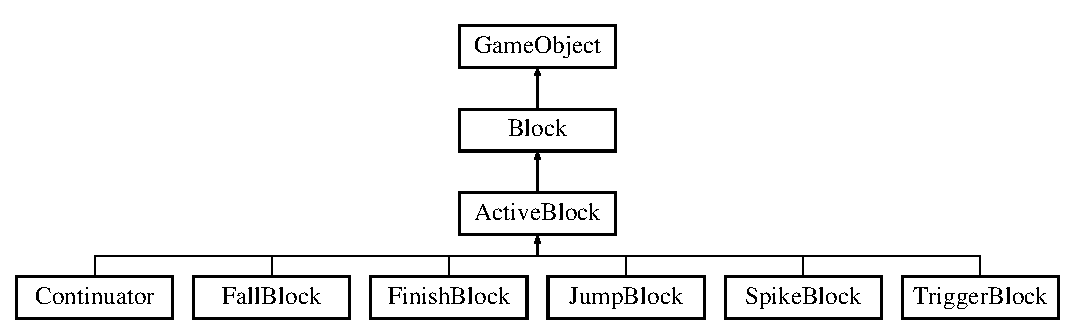
\includegraphics[height=4.000000cm]{class_active_block}
\end{center}
\end{figure}
\subsection*{Public Member Functions}
\begin{DoxyCompactItemize}
\item 
\hyperlink{class_active_block_a631a75f968d3d168ff61098545e8944b}{Active\+Block} (int x\+\_\+p, int y\+\_\+p, int w, int h, int amount\+Of\+Frames, std\+::string sprite\+Sheet, S\+D\+L\+\_\+\+Renderer $\ast$render)
\begin{DoxyCompactList}\small\item\em Constructor for \hyperlink{class_active_block}{Active\+Block}. \end{DoxyCompactList}\item 
\hypertarget{class_active_block_a9c94c51ce316a6697e17b08f124e74f8}{}virtual void {\bfseries activate} ()=0\label{class_active_block_a9c94c51ce316a6697e17b08f124e74f8}

\end{DoxyCompactItemize}
\subsection*{Protected Attributes}
\begin{DoxyCompactItemize}
\item 
\hypertarget{class_active_block_a4672b4f64f461acd3f6d1c701c7e55cd}{}bool {\bfseries active} \{false\}\label{class_active_block_a4672b4f64f461acd3f6d1c701c7e55cd}

\end{DoxyCompactItemize}
\subsection*{Additional Inherited Members}


\subsection{Constructor \& Destructor Documentation}
\hypertarget{class_active_block_a631a75f968d3d168ff61098545e8944b}{}\index{Active\+Block@{Active\+Block}!Active\+Block@{Active\+Block}}
\index{Active\+Block@{Active\+Block}!Active\+Block@{Active\+Block}}
\subsubsection[{Active\+Block(int x\+\_\+p, int y\+\_\+p, int w, int h, int amount\+Of\+Frames, std\+::string sprite\+Sheet, S\+D\+L\+\_\+\+Renderer $\ast$render)}]{\setlength{\rightskip}{0pt plus 5cm}Active\+Block\+::\+Active\+Block (
\begin{DoxyParamCaption}
\item[{int}]{x\+\_\+p, }
\item[{int}]{y\+\_\+p, }
\item[{int}]{w, }
\item[{int}]{h, }
\item[{int}]{amount\+Of\+Frames, }
\item[{std\+::string}]{sprite\+Sheet, }
\item[{S\+D\+L\+\_\+\+Renderer $\ast$}]{render}
\end{DoxyParamCaption}
)}\label{class_active_block_a631a75f968d3d168ff61098545e8944b}


Constructor for \hyperlink{class_active_block}{Active\+Block}. 


\begin{DoxyParams}{Parameters}
{\em x\+\_\+p} & x position of block \\
\hline
{\em y\+\_\+p} & y position of block \\
\hline
{\em w} & width of block \\
\hline
{\em h} & height of block \\
\hline
{\em amount\+Of\+Frames} & amount of frames in blocks spritesheet \\
\hline
{\em sprite\+Sheet} & location of spritesheet \\
\hline
{\em render} & renderer to draw to \\
\hline
\end{DoxyParams}


The documentation for this class was generated from the following files\+:\begin{DoxyCompactItemize}
\item 
/\+Users/lukas.\+vikstrom/\+Documents/\+T\+D\+P005/\+T\+D\+P005-\/\+Projekt/Active\+Block.\+h\item 
/\+Users/lukas.\+vikstrom/\+Documents/\+T\+D\+P005/\+T\+D\+P005-\/\+Projekt/Active\+Block.\+cc\end{DoxyCompactItemize}

\hypertarget{class_block}{}\section{Block Class Reference}
\label{class_block}\index{Block@{Block}}
Inheritance diagram for Block\+:\begin{figure}[H]
\begin{center}
\leavevmode
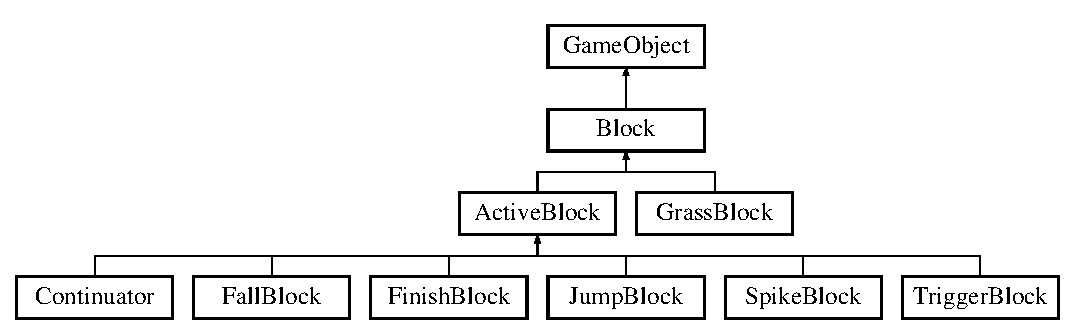
\includegraphics[height=4.000000cm]{class_block}
\end{center}
\end{figure}
\subsection*{Public Member Functions}
\begin{DoxyCompactItemize}
\item 
\hyperlink{class_block_afb6f1b926a0fc4d9024c101e40744ef5}{Block} (int x\+\_\+p, int y\+\_\+p, int w, int h, int amount\+Of\+Frames, std\+::string sprite\+Sheet, S\+D\+L\+\_\+\+Renderer $\ast$render)
\begin{DoxyCompactList}\small\item\em Constructor for \hyperlink{class_active_block}{Active\+Block}. \end{DoxyCompactList}\item 
\hypertarget{class_block_a7c02e05afb37da80875f17778916d6e5}{}virtual void {\bfseries update} (float const \&delta\+Time)\label{class_block_a7c02e05afb37da80875f17778916d6e5}

\item 
\hypertarget{class_block_a109153c2792ff5b4358bf3d39eb7132b}{}void {\bfseries will\+Collide} (std\+::vector$<$ \hyperlink{class_game_object}{Game\+Object} $\ast$ $>$ const \&objects)\label{class_block_a109153c2792ff5b4358bf3d39eb7132b}

\end{DoxyCompactItemize}
\subsection*{Additional Inherited Members}


\subsection{Constructor \& Destructor Documentation}
\hypertarget{class_block_afb6f1b926a0fc4d9024c101e40744ef5}{}\index{Block@{Block}!Block@{Block}}
\index{Block@{Block}!Block@{Block}}
\subsubsection[{Block(int x\+\_\+p, int y\+\_\+p, int w, int h, int amount\+Of\+Frames, std\+::string sprite\+Sheet, S\+D\+L\+\_\+\+Renderer $\ast$render)}]{\setlength{\rightskip}{0pt plus 5cm}Block\+::\+Block (
\begin{DoxyParamCaption}
\item[{int}]{x\+\_\+p, }
\item[{int}]{y\+\_\+p, }
\item[{int}]{w, }
\item[{int}]{h, }
\item[{int}]{amount\+Of\+Frames, }
\item[{std\+::string}]{sprite\+Sheet, }
\item[{S\+D\+L\+\_\+\+Renderer $\ast$}]{render}
\end{DoxyParamCaption}
)}\label{class_block_afb6f1b926a0fc4d9024c101e40744ef5}


Constructor for \hyperlink{class_active_block}{Active\+Block}. 


\begin{DoxyParams}{Parameters}
{\em x\+\_\+p} & x position of block \\
\hline
{\em y\+\_\+p} & y position of block \\
\hline
{\em w} & width of block \\
\hline
{\em h} & height of block \\
\hline
{\em amount\+Of\+Frames} & amount of frames in blocks spritesheet \\
\hline
{\em sprite\+Sheet} & location of spritesheet \\
\hline
{\em render} & renderer to draw to \\
\hline
\end{DoxyParams}


The documentation for this class was generated from the following files\+:\begin{DoxyCompactItemize}
\item 
/\+Users/lukas.\+vikstrom/\+Documents/\+T\+D\+P005/\+T\+D\+P005-\/\+Projekt/Block.\+h\item 
/\+Users/lukas.\+vikstrom/\+Documents/\+T\+D\+P005/\+T\+D\+P005-\/\+Projekt/Block.\+cc\end{DoxyCompactItemize}

\hypertarget{class_border}{}\section{Border Class Reference}
\label{class_border}\index{Border@{Border}}
Inheritance diagram for Border\+:\begin{figure}[H]
\begin{center}
\leavevmode
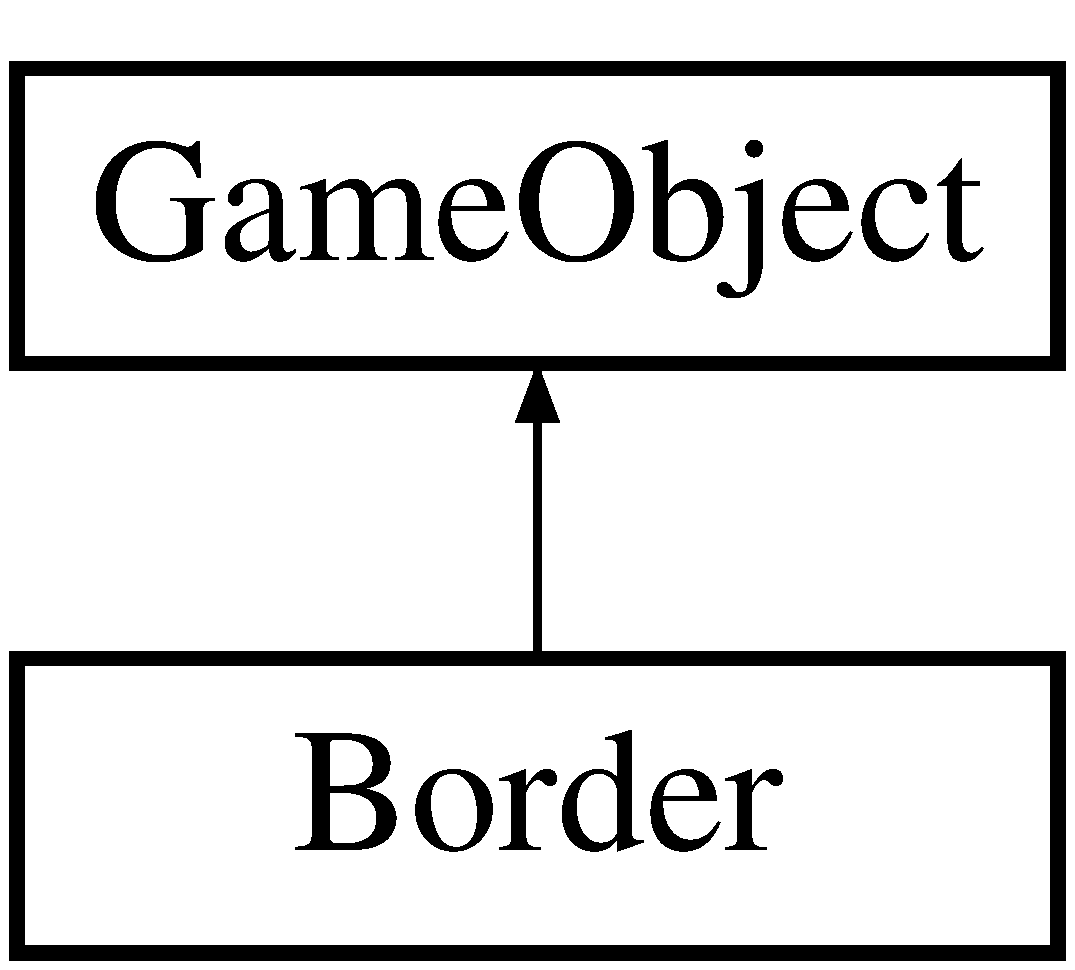
\includegraphics[height=2.000000cm]{class_border}
\end{center}
\end{figure}
\subsection*{Public Member Functions}
\begin{DoxyCompactItemize}
\item 
\hypertarget{class_border_a7eb54bc76259cb052bddf040f3f326c8}{}{\bfseries Border} (int x\+\_\+p, int y\+\_\+p, int w, int h, S\+D\+L\+\_\+\+Renderer $\ast$render)\label{class_border_a7eb54bc76259cb052bddf040f3f326c8}

\item 
\hypertarget{class_border_ab0fde818fc04af8ded1a0f14faf72bb0}{}void {\bfseries will\+Collide} (std\+::vector$<$ \hyperlink{class_game_object}{Game\+Object} $\ast$ $>$ const \&objects)\label{class_border_ab0fde818fc04af8ded1a0f14faf72bb0}

\item 
\hypertarget{class_border_af57e352dd3d0c47c27897161a59ce52b}{}void {\bfseries update} (float const \&delta\+Time)\label{class_border_af57e352dd3d0c47c27897161a59ce52b}

\end{DoxyCompactItemize}
\subsection*{Additional Inherited Members}


The documentation for this class was generated from the following files\+:\begin{DoxyCompactItemize}
\item 
/\+Users/lukas.\+vikstrom/\+Documents/\+T\+D\+P005/\+T\+D\+P005-\/\+Projekt/Border.\+h\item 
/\+Users/lukas.\+vikstrom/\+Documents/\+T\+D\+P005/\+T\+D\+P005-\/\+Projekt/Border.\+cc\end{DoxyCompactItemize}

\hypertarget{class_button}{}\section{Button Class Reference}
\label{class_button}\index{Button@{Button}}
\subsection*{Public Member Functions}
\begin{DoxyCompactItemize}
\item 
\hyperlink{class_button_a03de1bbd9fc5b177e3cd434f3ea85bae}{Button} (int x, int y, int w, int h, S\+D\+L\+\_\+\+Renderer $\ast$render, std\+::string button\+Image, std\+::string new\+Level\+Name, int new\+State\+Index)
\begin{DoxyCompactList}\small\item\em Constructor for \hyperlink{class_button}{Button} class. \end{DoxyCompactList}\item 
bool \hyperlink{class_button_a70d76c8c8a4e806f8a71771246cb18e2}{check\+For\+Click} (int x, int y)
\begin{DoxyCompactList}\small\item\em Checks for click on button. \end{DoxyCompactList}\end{DoxyCompactItemize}
\subsection*{Public Attributes}
\begin{DoxyCompactItemize}
\item 
\hypertarget{class_button_a51a8770221b4166852ebc54e8736c3f9}{}\hyperlink{class_sprite}{Sprite} $\ast$ {\bfseries sprite}\label{class_button_a51a8770221b4166852ebc54e8736c3f9}

\item 
\hypertarget{class_button_ae610e8cdd14cd5714c897e74605feda8}{}int {\bfseries click\+Statechange}\label{class_button_ae610e8cdd14cd5714c897e74605feda8}

\item 
\hypertarget{class_button_a4b7dcf42aa8dffdfce5ea3bc247d03a4}{}std\+::string {\bfseries click\+Value}\label{class_button_a4b7dcf42aa8dffdfce5ea3bc247d03a4}

\end{DoxyCompactItemize}


\subsection{Constructor \& Destructor Documentation}
\hypertarget{class_button_a03de1bbd9fc5b177e3cd434f3ea85bae}{}\index{Button@{Button}!Button@{Button}}
\index{Button@{Button}!Button@{Button}}
\subsubsection[{Button(int x, int y, int w, int h, S\+D\+L\+\_\+\+Renderer $\ast$render, std\+::string button\+Image, std\+::string new\+Level\+Name, int new\+State\+Index)}]{\setlength{\rightskip}{0pt plus 5cm}Button\+::\+Button (
\begin{DoxyParamCaption}
\item[{int}]{x, }
\item[{int}]{y, }
\item[{int}]{w, }
\item[{int}]{h, }
\item[{S\+D\+L\+\_\+\+Renderer $\ast$}]{render, }
\item[{std\+::string}]{button\+Image, }
\item[{std\+::string}]{new\+Level\+Name, }
\item[{int}]{new\+State\+Index}
\end{DoxyParamCaption}
)}\label{class_button_a03de1bbd9fc5b177e3cd434f3ea85bae}


Constructor for \hyperlink{class_button}{Button} class. 


\begin{DoxyParams}{Parameters}
{\em x} & x position of button \\
\hline
{\em y} & y position of button \\
\hline
{\em w} & width of button \\
\hline
{\em h} & height of button \\
\hline
{\em render} & renderer to draw to \\
\hline
{\em button\+Image} & location of image to draw to button \\
\hline
{\em new\+Level\+Name} & name of level to load on click \\
\hline
{\em new\+State\+Index} & index of state to change to \\
\hline
\end{DoxyParams}


\subsection{Member Function Documentation}
\hypertarget{class_button_a70d76c8c8a4e806f8a71771246cb18e2}{}\index{Button@{Button}!check\+For\+Click@{check\+For\+Click}}
\index{check\+For\+Click@{check\+For\+Click}!Button@{Button}}
\subsubsection[{check\+For\+Click(int x, int y)}]{\setlength{\rightskip}{0pt plus 5cm}bool Button\+::check\+For\+Click (
\begin{DoxyParamCaption}
\item[{int}]{x, }
\item[{int}]{y}
\end{DoxyParamCaption}
)}\label{class_button_a70d76c8c8a4e806f8a71771246cb18e2}


Checks for click on button. 

Compares x and y position of click with x and y position of button to see if the click occured on the button


\begin{DoxyParams}{Parameters}
{\em x} & x position of click \\
\hline
{\em y} & y position of click \\
\hline
\end{DoxyParams}


The documentation for this class was generated from the following files\+:\begin{DoxyCompactItemize}
\item 
/\+Users/lukas.\+vikstrom/\+Documents/\+T\+D\+P005/\+T\+D\+P005-\/\+Projekt/Button.\+h\item 
/\+Users/lukas.\+vikstrom/\+Documents/\+T\+D\+P005/\+T\+D\+P005-\/\+Projekt/Button.\+cc\end{DoxyCompactItemize}

\hypertarget{class_checkpoint}{}\section{Checkpoint Class Reference}
\label{class_checkpoint}\index{Checkpoint@{Checkpoint}}
Inheritance diagram for Checkpoint\+:\begin{figure}[H]
\begin{center}
\leavevmode
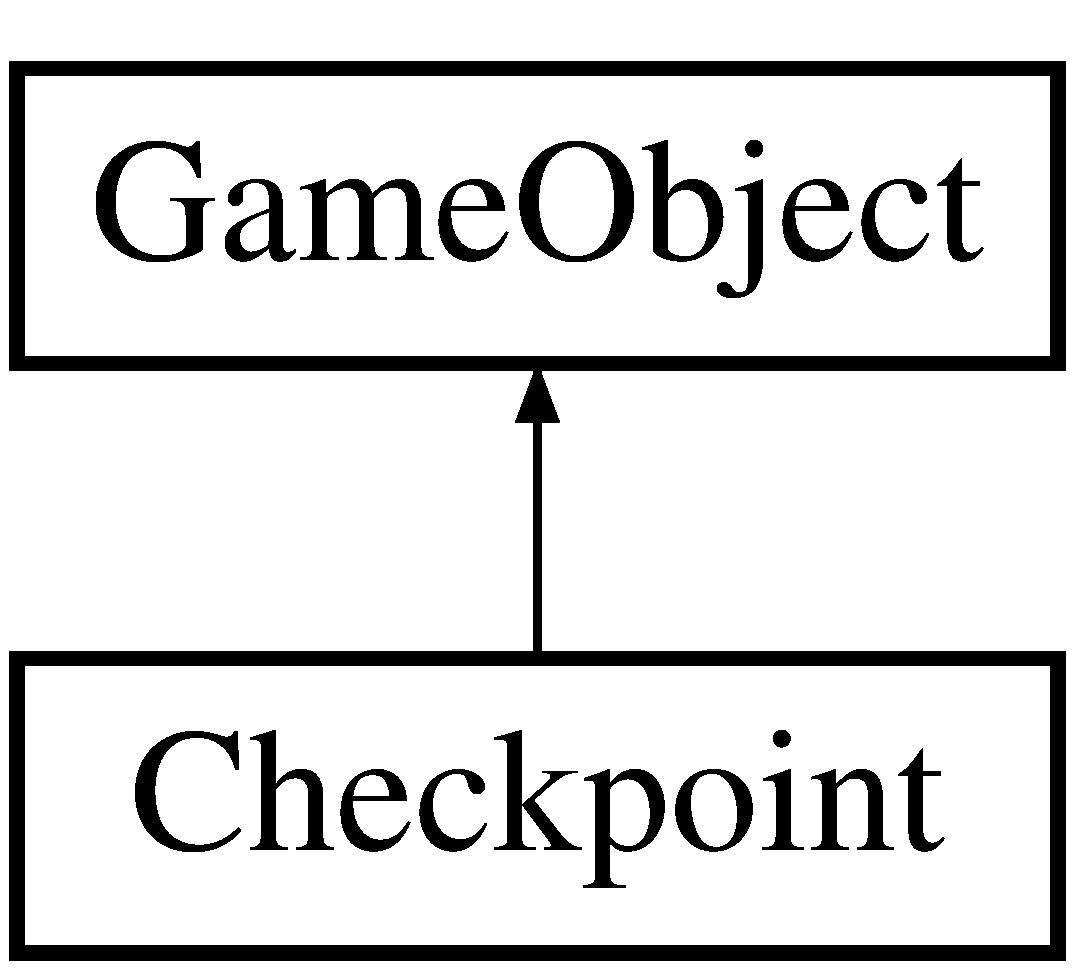
\includegraphics[height=2.000000cm]{class_checkpoint}
\end{center}
\end{figure}
\subsection*{Public Member Functions}
\begin{DoxyCompactItemize}
\item 
\hyperlink{class_checkpoint_ab5d42e643ba9db74db101152f0dd8885}{Checkpoint} (int x\+\_\+pos, int y\+\_\+pos, S\+D\+L\+\_\+\+Renderer $\ast$render)
\begin{DoxyCompactList}\small\item\em Constructor for \hyperlink{class_checkpoint}{Checkpoint}. \end{DoxyCompactList}\item 
\hypertarget{class_checkpoint_a7d23d012337203b8d36a92b53083b4fe}{}void {\bfseries update} (float const \&delta\+Time)\label{class_checkpoint_a7d23d012337203b8d36a92b53083b4fe}

\item 
\hypertarget{class_checkpoint_aea1ef559144b096ea6961012986b2a45}{}void {\bfseries will\+Collide} (std\+::vector$<$ \hyperlink{class_game_object}{Game\+Object} $\ast$ $>$ const \&objects)\label{class_checkpoint_aea1ef559144b096ea6961012986b2a45}

\end{DoxyCompactItemize}
\subsection*{Additional Inherited Members}


\subsection{Constructor \& Destructor Documentation}
\hypertarget{class_checkpoint_ab5d42e643ba9db74db101152f0dd8885}{}\index{Checkpoint@{Checkpoint}!Checkpoint@{Checkpoint}}
\index{Checkpoint@{Checkpoint}!Checkpoint@{Checkpoint}}
\subsubsection[{Checkpoint(int x\+\_\+pos, int y\+\_\+pos, S\+D\+L\+\_\+\+Renderer $\ast$render)}]{\setlength{\rightskip}{0pt plus 5cm}Checkpoint\+::\+Checkpoint (
\begin{DoxyParamCaption}
\item[{int}]{x\+\_\+pos, }
\item[{int}]{y\+\_\+pos, }
\item[{S\+D\+L\+\_\+\+Renderer $\ast$}]{renderer}
\end{DoxyParamCaption}
)}\label{class_checkpoint_ab5d42e643ba9db74db101152f0dd8885}


Constructor for \hyperlink{class_checkpoint}{Checkpoint}. 


\begin{DoxyParams}{Parameters}
{\em x\+Pos} & x position of checkpoint \\
\hline
{\em y\+Pos} & y position of checkpoint  renderer to draw to \\
\hline
\end{DoxyParams}


The documentation for this class was generated from the following files\+:\begin{DoxyCompactItemize}
\item 
/\+Users/lukas.\+vikstrom/\+Documents/\+T\+D\+P005/\+T\+D\+P005-\/\+Projekt/Checkpoint.\+h\item 
/\+Users/lukas.\+vikstrom/\+Documents/\+T\+D\+P005/\+T\+D\+P005-\/\+Projekt/Checkpoint.\+cc\end{DoxyCompactItemize}

\hypertarget{class_continuator}{}\section{Continuator Class Reference}
\label{class_continuator}\index{Continuator@{Continuator}}
Inheritance diagram for Continuator\+:\begin{figure}[H]
\begin{center}
\leavevmode
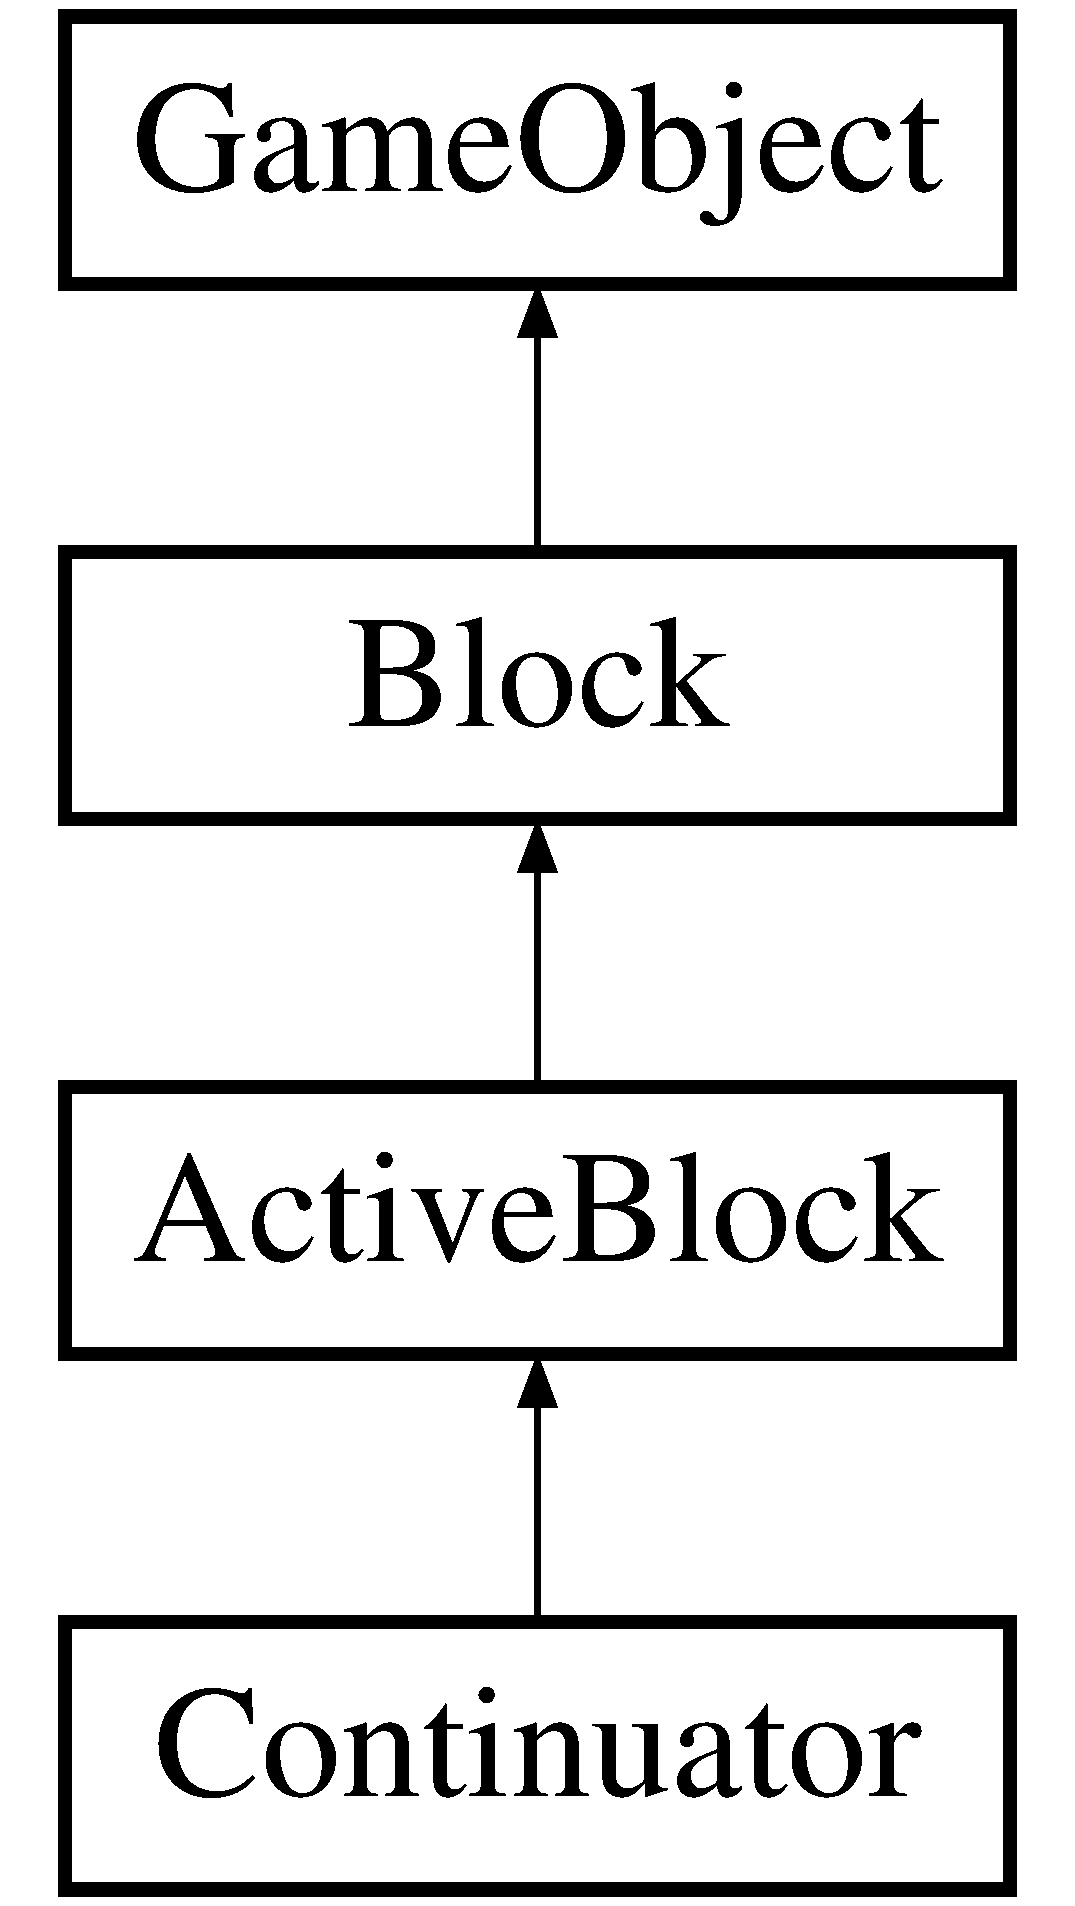
\includegraphics[height=4.000000cm]{class_continuator}
\end{center}
\end{figure}
\subsection*{Public Member Functions}
\begin{DoxyCompactItemize}
\item 
\hyperlink{class_continuator_a0983a0dece1cc4bdc524c6d81e0e2564}{Continuator} (int x, int y, S\+D\+L\+\_\+\+Renderer $\ast$render, std\+::string path)
\begin{DoxyCompactList}\small\item\em Constructor for \hyperlink{class_continuator}{Continuator} class. \end{DoxyCompactList}\item 
\hypertarget{class_continuator_a86b4d51415347063e6474297fe9f4656}{}void {\bfseries activate} ()\label{class_continuator_a86b4d51415347063e6474297fe9f4656}

\item 
\hypertarget{class_continuator_a02589158e4fdec4640069abede290848}{}std\+::string {\bfseries get\+Sub\+Level\+Path} ()\label{class_continuator_a02589158e4fdec4640069abede290848}

\end{DoxyCompactItemize}
\subsection*{Additional Inherited Members}


\subsection{Constructor \& Destructor Documentation}
\hypertarget{class_continuator_a0983a0dece1cc4bdc524c6d81e0e2564}{}\index{Continuator@{Continuator}!Continuator@{Continuator}}
\index{Continuator@{Continuator}!Continuator@{Continuator}}
\subsubsection[{Continuator(int x, int y, S\+D\+L\+\_\+\+Renderer $\ast$render, std\+::string path)}]{\setlength{\rightskip}{0pt plus 5cm}Continuator\+::\+Continuator (
\begin{DoxyParamCaption}
\item[{int}]{x, }
\item[{int}]{y, }
\item[{S\+D\+L\+\_\+\+Renderer $\ast$}]{renderer, }
\item[{std\+::string}]{path}
\end{DoxyParamCaption}
)}\label{class_continuator_a0983a0dece1cc4bdc524c6d81e0e2564}


Constructor for \hyperlink{class_continuator}{Continuator} class. 


\begin{DoxyParams}{Parameters}
{\em x} & x position of continuator \\
\hline
{\em y} & y position of continuator \\
\hline
{\em renderer} & renderer to draw to \\
\hline
{\em path} & location of new level to change to \\
\hline
\end{DoxyParams}


The documentation for this class was generated from the following files\+:\begin{DoxyCompactItemize}
\item 
/\+Users/lukas.\+vikstrom/\+Documents/\+T\+D\+P005/\+T\+D\+P005-\/\+Projekt/Continuator.\+h\item 
/\+Users/lukas.\+vikstrom/\+Documents/\+T\+D\+P005/\+T\+D\+P005-\/\+Projekt/Continuator.\+cc\end{DoxyCompactItemize}

\hypertarget{class_death_state}{}\section{Death\+State Class Reference}
\label{class_death_state}\index{Death\+State@{Death\+State}}
Inheritance diagram for Death\+State\+:\begin{figure}[H]
\begin{center}
\leavevmode
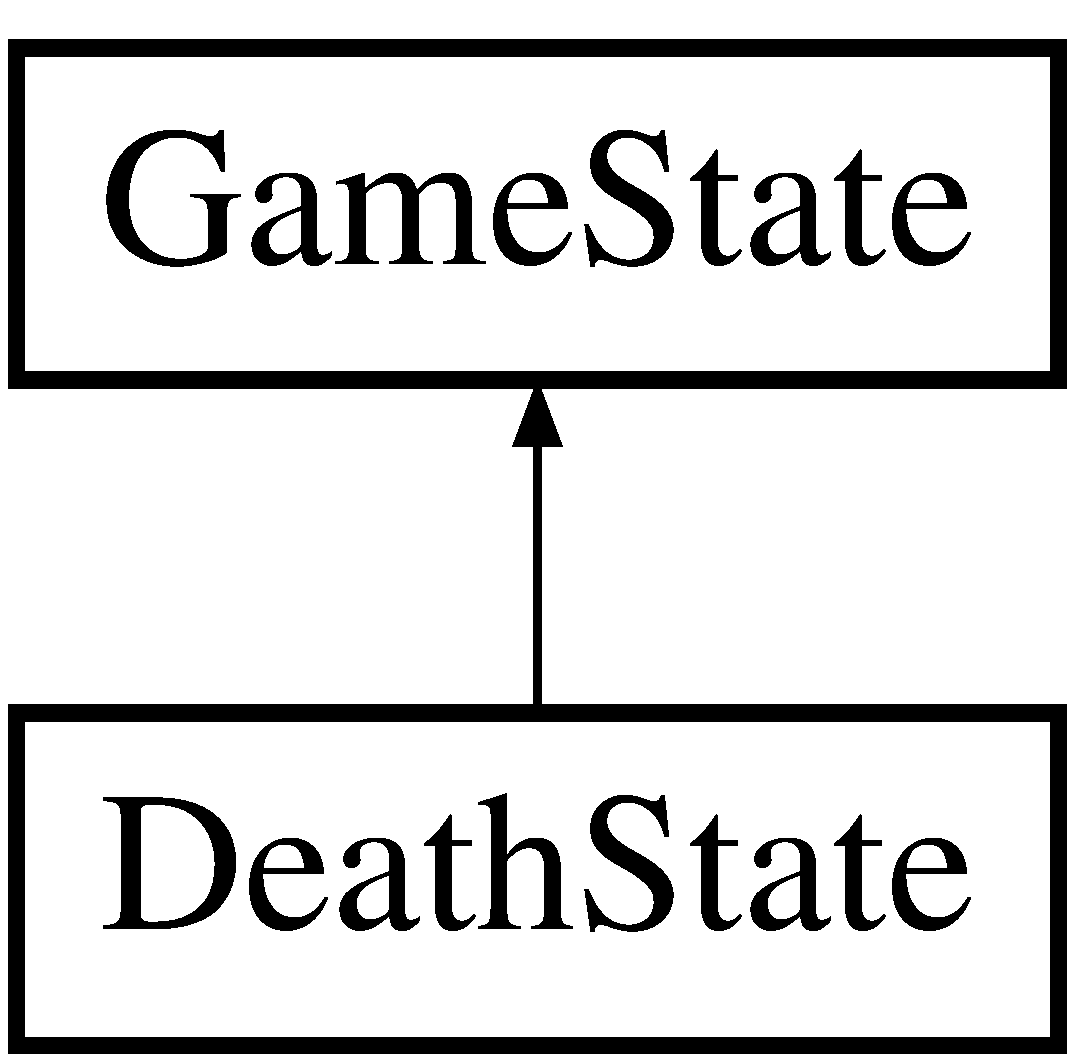
\includegraphics[height=2.000000cm]{class_death_state}
\end{center}
\end{figure}
\subsection*{Public Member Functions}
\begin{DoxyCompactItemize}
\item 
\hyperlink{class_death_state_a074c37ab4ffb4a2ccee2c6cb081aa77e}{Death\+State} (S\+D\+L\+\_\+\+Window $\ast$win, S\+D\+L\+\_\+\+Renderer $\ast$rend)
\begin{DoxyCompactList}\small\item\em Constructor for \hyperlink{class_death_state}{Death\+State}. \end{DoxyCompactList}\item 
void \hyperlink{class_death_state_adb482695885013654f7183792310c48e}{init} ()
\begin{DoxyCompactList}\small\item\em Initiator for Deathstate. \end{DoxyCompactList}\item 
void \hyperlink{class_death_state_a881a749aa4eebe860c7eeaa23e3a951c}{cleanup} ()
\begin{DoxyCompactList}\small\item\em Cleans up pointers. \end{DoxyCompactList}\item 
void \hyperlink{class_death_state_a9bafdb9541ae82810753fd7e30ca8c18}{update} (float const \&delta\+Time)
\begin{DoxyCompactList}\small\item\em Updator for \hyperlink{class_death_state}{Death\+State}. \end{DoxyCompactList}\item 
void \hyperlink{class_death_state_a99a1048e47fdd36407a344f1279abe17}{handle} (S\+D\+L\+\_\+\+Event event, float delta\+Time)
\begin{DoxyCompactList}\small\item\em Event handler for \hyperlink{class_death_state}{Death\+State}. \end{DoxyCompactList}\end{DoxyCompactItemize}
\subsection*{Public Attributes}
\begin{DoxyCompactItemize}
\item 
\hypertarget{class_death_state_a130e039dbfe19140caf1bc0238bc09fe}{}std\+::vector$<$ \hyperlink{class_button}{Button} $\ast$ $>$ {\bfseries menu\+Items}\label{class_death_state_a130e039dbfe19140caf1bc0238bc09fe}

\end{DoxyCompactItemize}
\subsection*{Additional Inherited Members}


\subsection{Constructor \& Destructor Documentation}
\hypertarget{class_death_state_a074c37ab4ffb4a2ccee2c6cb081aa77e}{}\index{Death\+State@{Death\+State}!Death\+State@{Death\+State}}
\index{Death\+State@{Death\+State}!Death\+State@{Death\+State}}
\subsubsection[{Death\+State(\+S\+D\+L\+\_\+\+Window $\ast$win, S\+D\+L\+\_\+\+Renderer $\ast$rend)}]{\setlength{\rightskip}{0pt plus 5cm}Death\+State\+::\+Death\+State (
\begin{DoxyParamCaption}
\item[{S\+D\+L\+\_\+\+Window $\ast$}]{win, }
\item[{S\+D\+L\+\_\+\+Renderer $\ast$}]{rend}
\end{DoxyParamCaption}
)}\label{class_death_state_a074c37ab4ffb4a2ccee2c6cb081aa77e}


Constructor for \hyperlink{class_death_state}{Death\+State}. 


\begin{DoxyParams}{Parameters}
{\em win} & window to draw to \\
\hline
{\em rend} & renderer to draw to \\
\hline
\end{DoxyParams}


\subsection{Member Function Documentation}
\hypertarget{class_death_state_a881a749aa4eebe860c7eeaa23e3a951c}{}\index{Death\+State@{Death\+State}!cleanup@{cleanup}}
\index{cleanup@{cleanup}!Death\+State@{Death\+State}}
\subsubsection[{cleanup()}]{\setlength{\rightskip}{0pt plus 5cm}void Death\+State\+::cleanup (
\begin{DoxyParamCaption}
{}
\end{DoxyParamCaption}
)\hspace{0.3cm}{\ttfamily [virtual]}}\label{class_death_state_a881a749aa4eebe860c7eeaa23e3a951c}


Cleans up pointers. 

Deletes the background pointer 

Implements \hyperlink{class_game_state}{Game\+State}.

\hypertarget{class_death_state_a99a1048e47fdd36407a344f1279abe17}{}\index{Death\+State@{Death\+State}!handle@{handle}}
\index{handle@{handle}!Death\+State@{Death\+State}}
\subsubsection[{handle(\+S\+D\+L\+\_\+\+Event event, float delta\+Time)}]{\setlength{\rightskip}{0pt plus 5cm}void Death\+State\+::handle (
\begin{DoxyParamCaption}
\item[{S\+D\+L\+\_\+\+Event}]{event, }
\item[{float}]{delta\+Time}
\end{DoxyParamCaption}
)\hspace{0.3cm}{\ttfamily [virtual]}}\label{class_death_state_a99a1048e47fdd36407a344f1279abe17}


Event handler for \hyperlink{class_death_state}{Death\+State}. 

Switches to play state if spacebar is pressed


\begin{DoxyParams}{Parameters}
{\em event} & event to handle \\
\hline
\end{DoxyParams}


Implements \hyperlink{class_game_state}{Game\+State}.

\hypertarget{class_death_state_adb482695885013654f7183792310c48e}{}\index{Death\+State@{Death\+State}!init@{init}}
\index{init@{init}!Death\+State@{Death\+State}}
\subsubsection[{init()}]{\setlength{\rightskip}{0pt plus 5cm}void Death\+State\+::init (
\begin{DoxyParamCaption}
{}
\end{DoxyParamCaption}
)\hspace{0.3cm}{\ttfamily [virtual]}}\label{class_death_state_adb482695885013654f7183792310c48e}


Initiator for Deathstate. 

Loads image to screen on death 

Implements \hyperlink{class_game_state}{Game\+State}.

\hypertarget{class_death_state_a9bafdb9541ae82810753fd7e30ca8c18}{}\index{Death\+State@{Death\+State}!update@{update}}
\index{update@{update}!Death\+State@{Death\+State}}
\subsubsection[{update(float const \&delta\+Time)}]{\setlength{\rightskip}{0pt plus 5cm}void Death\+State\+::update (
\begin{DoxyParamCaption}
\item[{float const \&}]{delta\+Time}
\end{DoxyParamCaption}
)\hspace{0.3cm}{\ttfamily [virtual]}}\label{class_death_state_a9bafdb9541ae82810753fd7e30ca8c18}


Updator for \hyperlink{class_death_state}{Death\+State}. 

Clears screen, draws the background, draws the buttons and renders it all on update 

Implements \hyperlink{class_game_state}{Game\+State}.



The documentation for this class was generated from the following files\+:\begin{DoxyCompactItemize}
\item 
/\+Users/lukas.\+vikstrom/\+Documents/\+T\+D\+P005/\+T\+D\+P005-\/\+Projekt/Death\+State.\+h\item 
/\+Users/lukas.\+vikstrom/\+Documents/\+T\+D\+P005/\+T\+D\+P005-\/\+Projekt/Death\+State.\+cc\end{DoxyCompactItemize}

\hypertarget{class_enemy}{}\section{Enemy Class Reference}
\label{class_enemy}\index{Enemy@{Enemy}}
Inheritance diagram for Enemy\+:\begin{figure}[H]
\begin{center}
\leavevmode
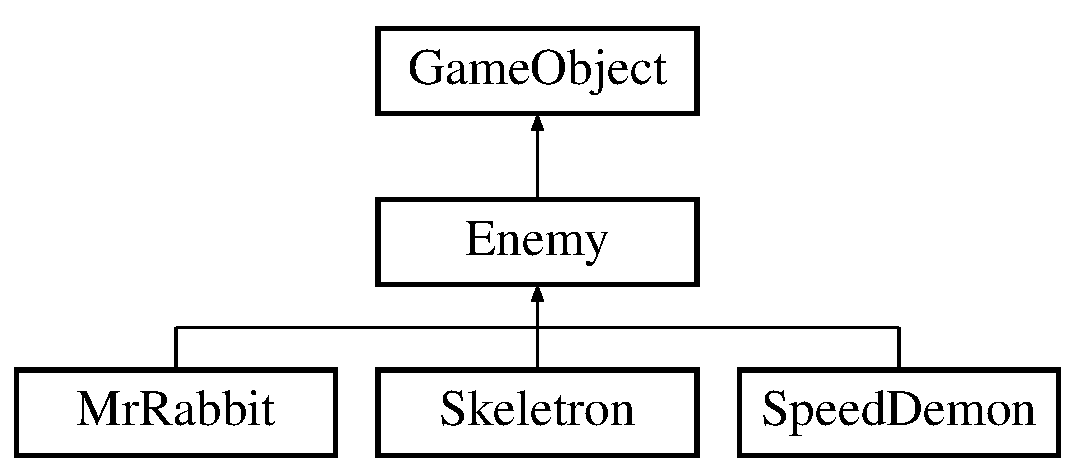
\includegraphics[height=3.000000cm]{class_enemy}
\end{center}
\end{figure}
\subsection*{Public Member Functions}
\begin{DoxyCompactItemize}
\item 
\hyperlink{class_enemy_a82d8148ea7ca6fb9a77112014bb6682c}{Enemy} (int x\+\_\+p, int y\+\_\+p, int w, int h, int amount\+Of\+Frames, std\+::string sprite\+Sheet, S\+D\+L\+\_\+\+Renderer $\ast$render, \hyperlink{class_player}{Player} $\ast$player\+\_\+ptr)
\begin{DoxyCompactList}\small\item\em Constructor for \hyperlink{class_active_block}{Active\+Block}. \end{DoxyCompactList}\item 
\hypertarget{class_enemy_a4b883487df30d884389546d6d152a21b}{}virtual void {\bfseries decide\+Action} ()=0\label{class_enemy_a4b883487df30d884389546d6d152a21b}

\item 
void \hyperlink{class_enemy_a40d054c26a502f7dbd310f4b1fb51c5c}{move\+Left} ()
\begin{DoxyCompactList}\small\item\em Moves to the left. \end{DoxyCompactList}\item 
void \hyperlink{class_enemy_ab7fd09209895cb57198408f32cac8ce9}{move\+Right} ()
\begin{DoxyCompactList}\small\item\em Moves to the right. \end{DoxyCompactList}\end{DoxyCompactItemize}
\subsection*{Protected Attributes}
\begin{DoxyCompactItemize}
\item 
\hypertarget{class_enemy_ada809d9584f684943180df738276cf5d}{}\hyperlink{class_player}{Player} $\ast$ {\bfseries player}\label{class_enemy_ada809d9584f684943180df738276cf5d}

\end{DoxyCompactItemize}
\subsection*{Additional Inherited Members}


\subsection{Constructor \& Destructor Documentation}
\hypertarget{class_enemy_a82d8148ea7ca6fb9a77112014bb6682c}{}\index{Enemy@{Enemy}!Enemy@{Enemy}}
\index{Enemy@{Enemy}!Enemy@{Enemy}}
\subsubsection[{Enemy(int x\+\_\+p, int y\+\_\+p, int w, int h, int amount\+Of\+Frames, std\+::string sprite\+Sheet, S\+D\+L\+\_\+\+Renderer $\ast$render, Player $\ast$player\+\_\+ptr)}]{\setlength{\rightskip}{0pt plus 5cm}Enemy\+::\+Enemy (
\begin{DoxyParamCaption}
\item[{int}]{x\+\_\+p, }
\item[{int}]{y\+\_\+p, }
\item[{int}]{w, }
\item[{int}]{h, }
\item[{int}]{amount\+Of\+Frames, }
\item[{std\+::string}]{sprite\+Sheet, }
\item[{S\+D\+L\+\_\+\+Renderer $\ast$}]{render, }
\item[{{\bf Player} $\ast$}]{player\+\_\+ptr}
\end{DoxyParamCaption}
)}\label{class_enemy_a82d8148ea7ca6fb9a77112014bb6682c}


Constructor for \hyperlink{class_active_block}{Active\+Block}. 


\begin{DoxyParams}{Parameters}
{\em x\+\_\+p} & x position of block \\
\hline
{\em y\+\_\+p} & y position of block \\
\hline
{\em w} & width of block \\
\hline
{\em h} & height of block \\
\hline
{\em amount\+Of\+Frames} & amount of frames in blocks spritesheet \\
\hline
{\em sprite\+Sheet} & location of spritesheet \\
\hline
{\em render} & renderer to draw to \\
\hline
{\em player\+\_\+ptr} & Pointer to the active player \\
\hline
\end{DoxyParams}


\subsection{Member Function Documentation}
\hypertarget{class_enemy_a40d054c26a502f7dbd310f4b1fb51c5c}{}\index{Enemy@{Enemy}!move\+Left@{move\+Left}}
\index{move\+Left@{move\+Left}!Enemy@{Enemy}}
\subsubsection[{move\+Left()}]{\setlength{\rightskip}{0pt plus 5cm}void Enemy\+::move\+Left (
\begin{DoxyParamCaption}
{}
\end{DoxyParamCaption}
)}\label{class_enemy_a40d054c26a502f7dbd310f4b1fb51c5c}


Moves to the left. 

Updates objects x position to move left on the game screen \hypertarget{class_enemy_ab7fd09209895cb57198408f32cac8ce9}{}\index{Enemy@{Enemy}!move\+Right@{move\+Right}}
\index{move\+Right@{move\+Right}!Enemy@{Enemy}}
\subsubsection[{move\+Right()}]{\setlength{\rightskip}{0pt plus 5cm}void Enemy\+::move\+Right (
\begin{DoxyParamCaption}
{}
\end{DoxyParamCaption}
)}\label{class_enemy_ab7fd09209895cb57198408f32cac8ce9}


Moves to the right. 

Updates objects x position to move right on the game screen 

The documentation for this class was generated from the following files\+:\begin{DoxyCompactItemize}
\item 
/\+Users/lukas.\+vikstrom/\+Documents/\+T\+D\+P005/\+T\+D\+P005-\/\+Projekt/Enemy.\+h\item 
/\+Users/lukas.\+vikstrom/\+Documents/\+T\+D\+P005/\+T\+D\+P005-\/\+Projekt/Enemy.\+cc\end{DoxyCompactItemize}

\hypertarget{class_fall_block}{}\section{Fall\+Block Class Reference}
\label{class_fall_block}\index{Fall\+Block@{Fall\+Block}}
Inheritance diagram for Fall\+Block\+:\begin{figure}[H]
\begin{center}
\leavevmode
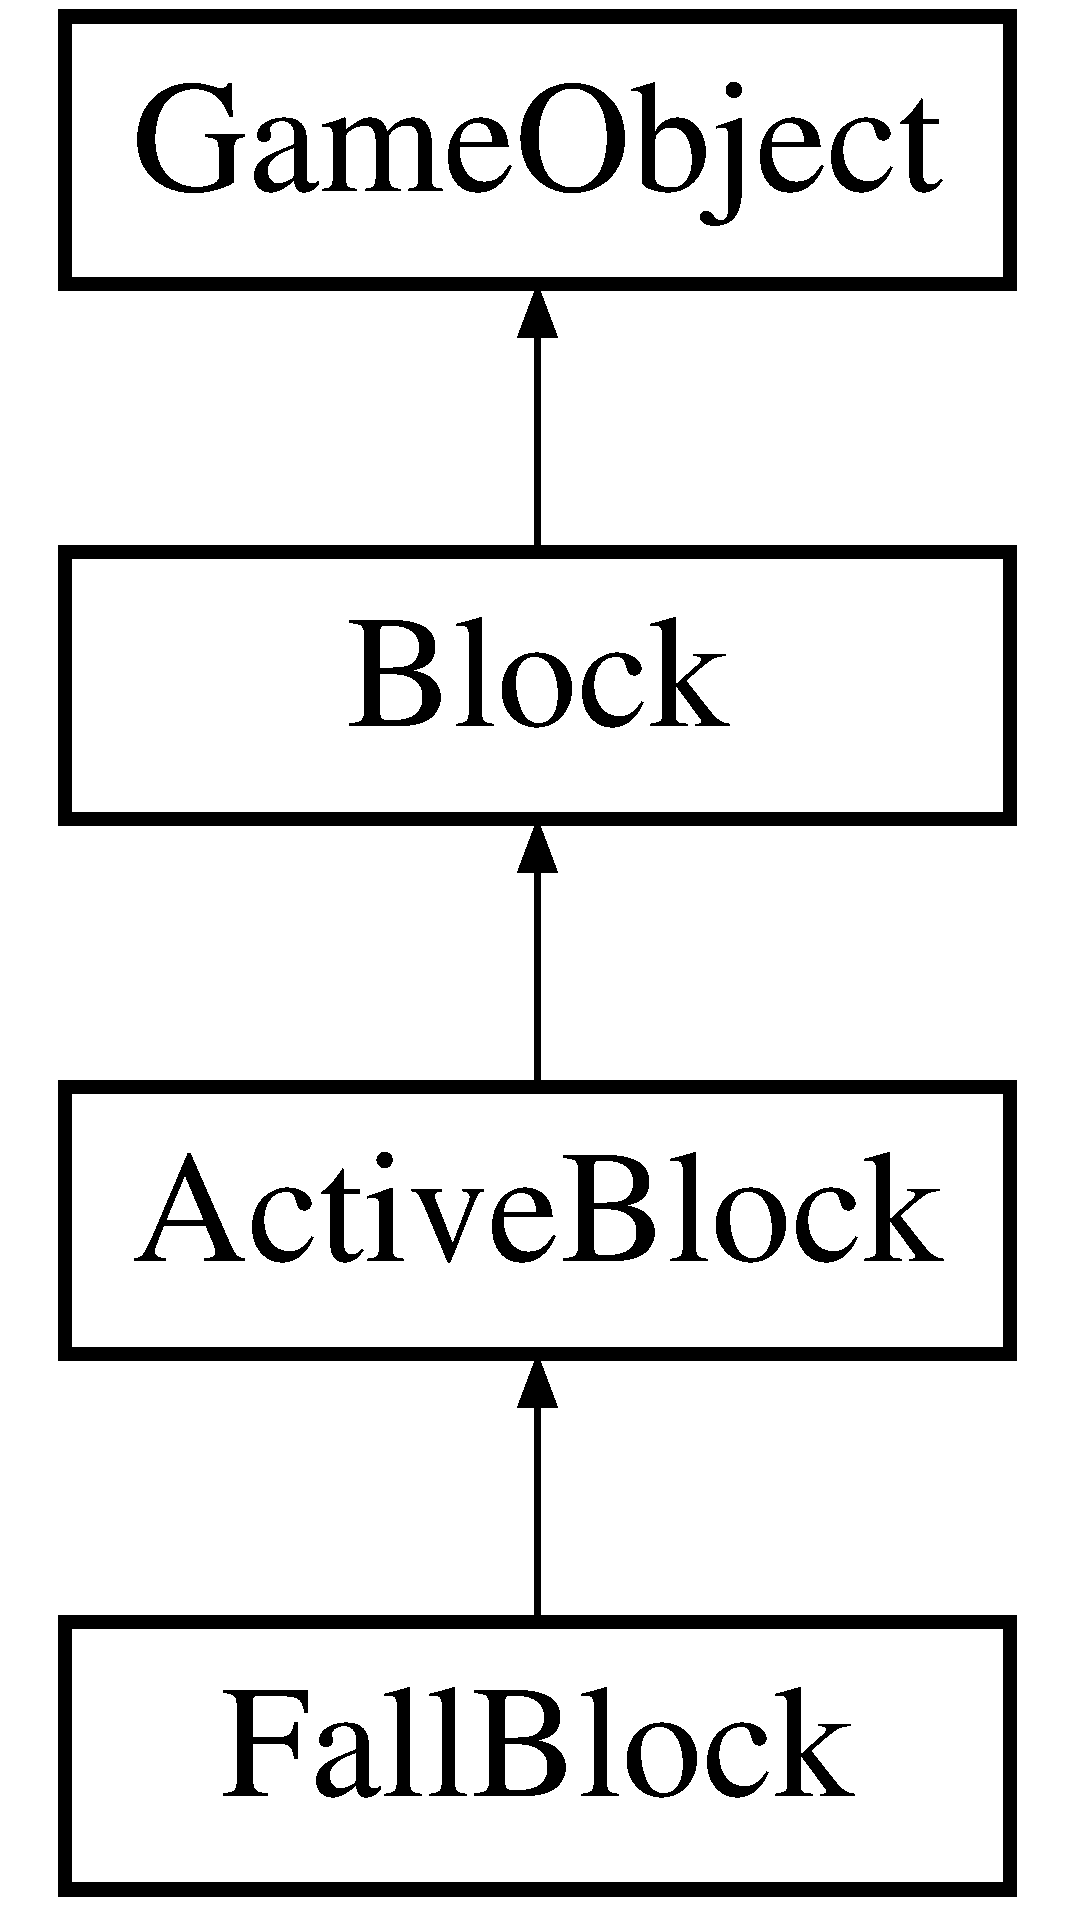
\includegraphics[height=4.000000cm]{class_fall_block}
\end{center}
\end{figure}
\subsection*{Public Member Functions}
\begin{DoxyCompactItemize}
\item 
\hyperlink{class_fall_block_a1e025d052d33b87556953efdba8ab769}{Fall\+Block} (int x\+\_\+pos, int y\+\_\+pos, S\+D\+L\+\_\+\+Renderer $\ast$render, bool acti)
\begin{DoxyCompactList}\small\item\em Constructor for \hyperlink{class_fall_block}{Fall\+Block}. \end{DoxyCompactList}\item 
void \hyperlink{class_fall_block_aba7d07cfa6d05202e31bc388aff89256}{activate} ()
\begin{DoxyCompactList}\small\item\em Activator for \hyperlink{class_fall_block}{Fall\+Block}. \end{DoxyCompactList}\item 
void \hyperlink{class_fall_block_a91e9a9e851ebf5322200f8136235528b}{update} (float const \&delta\+Time)
\begin{DoxyCompactList}\small\item\em Updator for \hyperlink{class_fall_block}{Fall\+Block}. \end{DoxyCompactList}\end{DoxyCompactItemize}
\subsection*{Additional Inherited Members}


\subsection{Constructor \& Destructor Documentation}
\hypertarget{class_fall_block_a1e025d052d33b87556953efdba8ab769}{}\index{Fall\+Block@{Fall\+Block}!Fall\+Block@{Fall\+Block}}
\index{Fall\+Block@{Fall\+Block}!Fall\+Block@{Fall\+Block}}
\subsubsection[{Fall\+Block(int x\+\_\+pos, int y\+\_\+pos, S\+D\+L\+\_\+\+Renderer $\ast$render, bool acti)}]{\setlength{\rightskip}{0pt plus 5cm}Fall\+Block\+::\+Fall\+Block (
\begin{DoxyParamCaption}
\item[{int}]{x\+\_\+pos, }
\item[{int}]{y\+\_\+pos, }
\item[{S\+D\+L\+\_\+\+Renderer $\ast$}]{render, }
\item[{bool}]{acti}
\end{DoxyParamCaption}
)}\label{class_fall_block_a1e025d052d33b87556953efdba8ab769}


Constructor for \hyperlink{class_fall_block}{Fall\+Block}. 


\begin{DoxyParams}{Parameters}
{\em x\+Pos} & x position of block \\
\hline
{\em y\+Pos} & y position of block \\
\hline
{\em render} & renderer to draw to \\
\hline
{\em acti} & states if block is activatable by player \\
\hline
\end{DoxyParams}


\subsection{Member Function Documentation}
\hypertarget{class_fall_block_aba7d07cfa6d05202e31bc388aff89256}{}\index{Fall\+Block@{Fall\+Block}!activate@{activate}}
\index{activate@{activate}!Fall\+Block@{Fall\+Block}}
\subsubsection[{activate()}]{\setlength{\rightskip}{0pt plus 5cm}void Fall\+Block\+::activate (
\begin{DoxyParamCaption}
{}
\end{DoxyParamCaption}
)\hspace{0.3cm}{\ttfamily [virtual]}}\label{class_fall_block_aba7d07cfa6d05202e31bc388aff89256}


Activator for \hyperlink{class_fall_block}{Fall\+Block}. 

Makes the block active and changes its type to the intended one 

Implements \hyperlink{class_active_block}{Active\+Block}.

\hypertarget{class_fall_block_a91e9a9e851ebf5322200f8136235528b}{}\index{Fall\+Block@{Fall\+Block}!update@{update}}
\index{update@{update}!Fall\+Block@{Fall\+Block}}
\subsubsection[{update(float const \&delta\+Time)}]{\setlength{\rightskip}{0pt plus 5cm}void Fall\+Block\+::update (
\begin{DoxyParamCaption}
\item[{float const \&}]{delta\+Time}
\end{DoxyParamCaption}
)\hspace{0.3cm}{\ttfamily [virtual]}}\label{class_fall_block_a91e9a9e851ebf5322200f8136235528b}


Updator for \hyperlink{class_fall_block}{Fall\+Block}. 

Makes the block fall if it\textquotesingle{}s active 

Reimplemented from \hyperlink{class_block}{Block}.



The documentation for this class was generated from the following files\+:\begin{DoxyCompactItemize}
\item 
/\+Users/lukas.\+vikstrom/\+Documents/\+T\+D\+P005/\+T\+D\+P005-\/\+Projekt/Fall\+Block.\+h\item 
/\+Users/lukas.\+vikstrom/\+Documents/\+T\+D\+P005/\+T\+D\+P005-\/\+Projekt/Fall\+Block.\+cc\end{DoxyCompactItemize}

\hypertarget{class_finish_block}{}\section{Finish\+Block Class Reference}
\label{class_finish_block}\index{Finish\+Block@{Finish\+Block}}
Inheritance diagram for Finish\+Block\+:\begin{figure}[H]
\begin{center}
\leavevmode
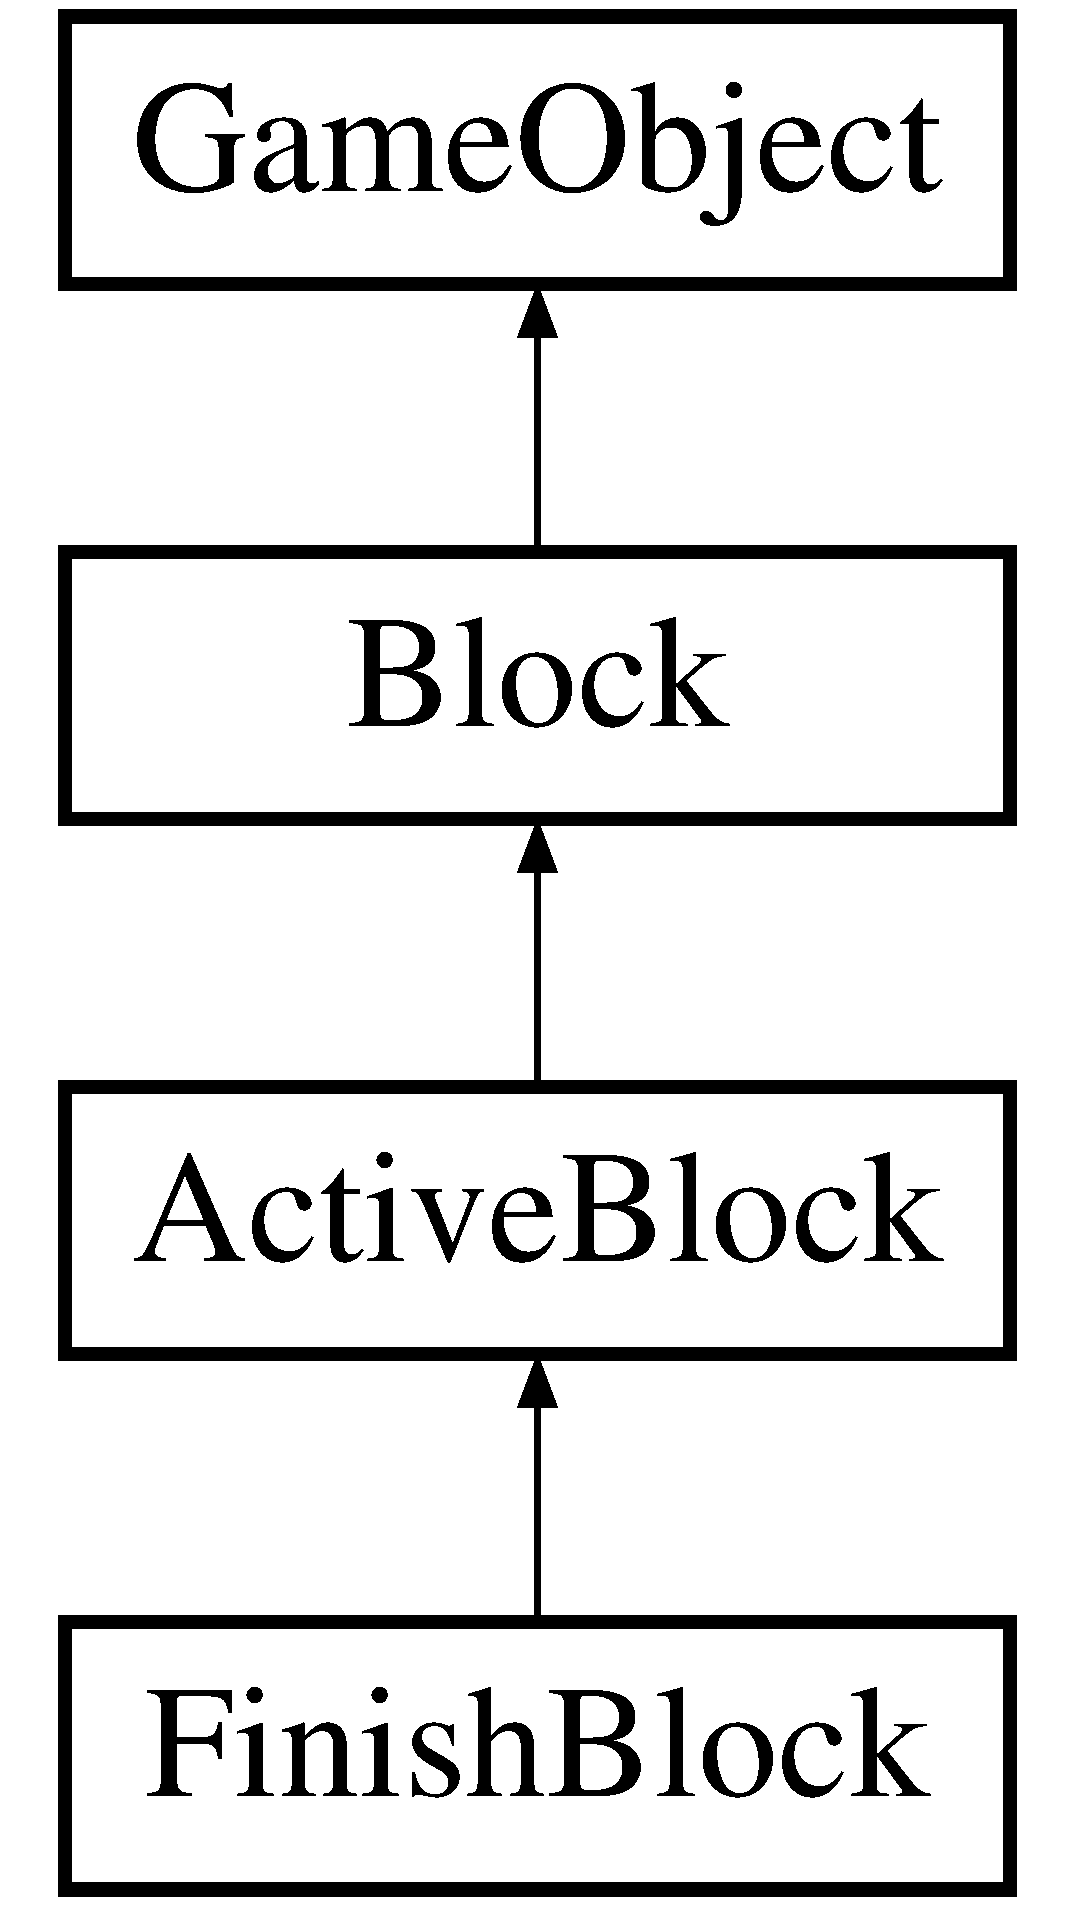
\includegraphics[height=4.000000cm]{class_finish_block}
\end{center}
\end{figure}
\subsection*{Public Member Functions}
\begin{DoxyCompactItemize}
\item 
\hypertarget{class_finish_block_a98778169bc154ec4f534f67b2424ba95}{}{\bfseries Finish\+Block} (int x\+\_\+pos, int y\+\_\+pos, S\+D\+L\+\_\+\+Renderer $\ast$render, int visible\+On\+Start)\label{class_finish_block_a98778169bc154ec4f534f67b2424ba95}

\item 
\hypertarget{class_finish_block_a8309ee02694113a7b2f7bcc9123009aa}{}void {\bfseries activate} ()\label{class_finish_block_a8309ee02694113a7b2f7bcc9123009aa}

\item 
\hypertarget{class_finish_block_a530bc99f20b0763aa56532b7307aecf9}{}void {\bfseries de\+Activate} ()\label{class_finish_block_a530bc99f20b0763aa56532b7307aecf9}

\end{DoxyCompactItemize}
\subsection*{Additional Inherited Members}


The documentation for this class was generated from the following files\+:\begin{DoxyCompactItemize}
\item 
/\+Users/lukas.\+vikstrom/\+Documents/\+T\+D\+P005/\+T\+D\+P005-\/\+Projekt/Finish\+Block.\+h\item 
/\+Users/lukas.\+vikstrom/\+Documents/\+T\+D\+P005/\+T\+D\+P005-\/\+Projekt/Finish\+Block.\+cc\end{DoxyCompactItemize}

\hypertarget{class_game_object}{}\section{Game\+Object Class Reference}
\label{class_game_object}\index{Game\+Object@{Game\+Object}}
Inheritance diagram for Game\+Object\+:\begin{figure}[H]
\begin{center}
\leavevmode
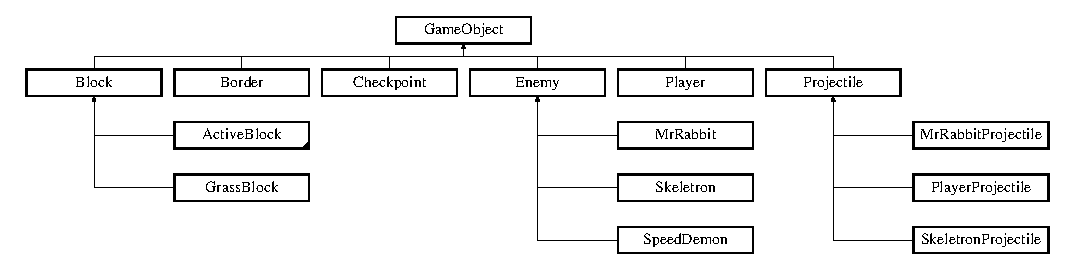
\includegraphics[height=3.174603cm]{class_game_object}
\end{center}
\end{figure}
\subsection*{Public Member Functions}
\begin{DoxyCompactItemize}
\item 
\hyperlink{class_game_object_a20572b6ae69d08069628c089cf443579}{Game\+Object} (int x\+\_\+p, int y\+\_\+p, int w, int h, int amount\+Of\+Frames, std\+::string sprite\+Sheet, S\+D\+L\+\_\+\+Renderer $\ast$render)
\begin{DoxyCompactList}\small\item\em Constructor for \hyperlink{class_game_object}{Game\+Object}. \end{DoxyCompactList}\item 
\hypertarget{class_game_object_a7acc9f88334654fefe7c8af8be0c49cf}{}virtual void {\bfseries handle\+Collision} (std\+::vector$<$ std\+::pair$<$ \hyperlink{class_game_object}{Game\+Object} $\ast$, std\+::array$<$ std\+::string, 4 $>$ $>$ $>$ colliding\+Objects)=0\label{class_game_object_a7acc9f88334654fefe7c8af8be0c49cf}

\item 
\hypertarget{class_game_object_a27ab44c46dedfd391e439bddd13fdb75}{}virtual void {\bfseries will\+Collide} (std\+::vector$<$ \hyperlink{class_game_object}{Game\+Object} $\ast$ $>$ const \&objects)=0\label{class_game_object_a27ab44c46dedfd391e439bddd13fdb75}

\item 
\hypertarget{class_game_object_a11b8c66b3432576a77c50a8dc67ca95b}{}virtual void {\bfseries update} (float const \&delta\+Time)=0\label{class_game_object_a11b8c66b3432576a77c50a8dc67ca95b}

\item 
\hypertarget{class_game_object_a113b5e4d1e22c04b6f72c191286bd4f7}{}virtual void {\bfseries create\+Object} (std\+::vector$<$ \hyperlink{class_game_object}{Game\+Object} $\ast$ $>$ \&map\+\_\+objects)\label{class_game_object_a113b5e4d1e22c04b6f72c191286bd4f7}

\item 
void \hyperlink{class_game_object_a5334326f93fee2f6bd0b5cb0cea1f858}{update\+Position} ()
\begin{DoxyCompactList}\small\item\em Updates position. \end{DoxyCompactList}\item 
void \hyperlink{class_game_object_a8c19716181d12dd100bd5fde8fdb09bb}{take\+Dmg} ()
\begin{DoxyCompactList}\small\item\em Changes objects hp or kills it. \end{DoxyCompactList}\item 
void \hyperlink{class_game_object_a14cc28b2288fcafb347360d9baaf6f15}{update\+Gravity} (float const \&delta\+Time)
\begin{DoxyCompactList}\small\item\em Updates position based on gravity calculation. \end{DoxyCompactList}\item 
bool \hyperlink{class_game_object_aa140af3122d8b8dd4b082774a9f879c4}{intersect} (\hyperlink{class_game_object}{Game\+Object} $\ast$const \&a, std\+::array$<$ std\+::string, 4 $>$ \&result)
\begin{DoxyCompactList}\small\item\em Checks for intersection and returns if a collision has occurred. \end{DoxyCompactList}\item 
void \hyperlink{class_game_object_af54107b086de78b1fc6190088bdfb468}{kill} ()
\begin{DoxyCompactList}\small\item\em Kills the object. \end{DoxyCompactList}\item 
\hypertarget{class_game_object_a3a4916a49e3dcad9c2f890a4ea41758f}{}std\+::string {\bfseries get\+Type} () const \label{class_game_object_a3a4916a49e3dcad9c2f890a4ea41758f}

\item 
\hypertarget{class_game_object_a29bf50e009a530b444f8157dc20c65df}{}double {\bfseries get\+X\+Vel} () const \label{class_game_object_a29bf50e009a530b444f8157dc20c65df}

\item 
\hypertarget{class_game_object_a6e0690e683eff5b5fa866161f2f17d02}{}void {\bfseries set\+X\+Vel} (int const \&new\+\_\+xvel)\label{class_game_object_a6e0690e683eff5b5fa866161f2f17d02}

\item 
\hypertarget{class_game_object_adee1a9a33c76236c072f22e6049e9985}{}double {\bfseries get\+Y\+Vel} () const \label{class_game_object_adee1a9a33c76236c072f22e6049e9985}

\item 
\hypertarget{class_game_object_a661db91109a8ef1a97c2aab8e65b063b}{}void {\bfseries set\+Y\+Vel} (int const \&new\+\_\+yvel)\label{class_game_object_a661db91109a8ef1a97c2aab8e65b063b}

\item 
\hypertarget{class_game_object_ace6182e9f11f78c860309e80c02f02a4}{}bool {\bfseries get\+Dying} () const \label{class_game_object_ace6182e9f11f78c860309e80c02f02a4}

\item 
\hypertarget{class_game_object_a7f5572a077957d6f96d45d70d9b24880}{}int {\bfseries get\+Direction} () const \label{class_game_object_a7f5572a077957d6f96d45d70d9b24880}

\item 
\hypertarget{class_game_object_ad46ad4ff6ddd72d309d6fbbcd8805e30}{}int {\bfseries get\+Health} () const \label{class_game_object_ad46ad4ff6ddd72d309d6fbbcd8805e30}

\end{DoxyCompactItemize}
\subsection*{Public Attributes}
\begin{DoxyCompactItemize}
\item 
\hypertarget{class_game_object_a7064902ef403216ffe8ec2503a5b70bb}{}int {\bfseries x\+Pos}\label{class_game_object_a7064902ef403216ffe8ec2503a5b70bb}

\item 
\hypertarget{class_game_object_a6e409956cceec4c73d33564a6c30f18d}{}int {\bfseries y\+Pos}\label{class_game_object_a6e409956cceec4c73d33564a6c30f18d}

\item 
\hypertarget{class_game_object_aa1e23b643890c0bdc3b6d8512bb3422c}{}bool {\bfseries collided\+This\+Update} \{false\}\label{class_game_object_aa1e23b643890c0bdc3b6d8512bb3422c}

\item 
\hypertarget{class_game_object_a00fecd21a33c990c4132f6f8e886135f}{}\hyperlink{class_sprite}{Sprite} $\ast$ {\bfseries sprite}\label{class_game_object_a00fecd21a33c990c4132f6f8e886135f}

\end{DoxyCompactItemize}
\subsection*{Protected Attributes}
\begin{DoxyCompactItemize}
\item 
\hypertarget{class_game_object_a800205ed5a8c1e75727157ca2fc05e3a}{}int {\bfseries direction} \{1\}\label{class_game_object_a800205ed5a8c1e75727157ca2fc05e3a}

\item 
\hypertarget{class_game_object_a583d4de3d4a6c8c5e6bdd99dce383854}{}bool {\bfseries die\+Next\+Update} \{false\}\label{class_game_object_a583d4de3d4a6c8c5e6bdd99dce383854}

\item 
\hypertarget{class_game_object_aec7475f944e4d3ed46953c452513929f}{}double {\bfseries y\+Vel} \{0\}\label{class_game_object_aec7475f944e4d3ed46953c452513929f}

\item 
\hypertarget{class_game_object_a8ec343c42814fd6f61cb32feb9e060cb}{}double {\bfseries x\+Vel} \{0\}\label{class_game_object_a8ec343c42814fd6f61cb32feb9e060cb}

\item 
\hypertarget{class_game_object_a35313c55194b2c2c42270bbc97306b76}{}int {\bfseries health} \{1\}\label{class_game_object_a35313c55194b2c2c42270bbc97306b76}

\item 
\hypertarget{class_game_object_aa1ece14d94ea4cdb1bb497889bdf70a3}{}double {\bfseries air\+Time} \{0\}\label{class_game_object_aa1ece14d94ea4cdb1bb497889bdf70a3}

\item 
\hypertarget{class_game_object_a15cb8c7ceed697b8f7eefe79675875dd}{}std\+::string {\bfseries type} \{\char`\"{}Game\+Object\char`\"{}\}\label{class_game_object_a15cb8c7ceed697b8f7eefe79675875dd}

\end{DoxyCompactItemize}


\subsection{Constructor \& Destructor Documentation}
\hypertarget{class_game_object_a20572b6ae69d08069628c089cf443579}{}\index{Game\+Object@{Game\+Object}!Game\+Object@{Game\+Object}}
\index{Game\+Object@{Game\+Object}!Game\+Object@{Game\+Object}}
\subsubsection[{Game\+Object(int x\+\_\+p, int y\+\_\+p, int w, int h, int amount\+Of\+Frames, std\+::string sprite\+Sheet, S\+D\+L\+\_\+\+Renderer $\ast$render)}]{\setlength{\rightskip}{0pt plus 5cm}Game\+Object\+::\+Game\+Object (
\begin{DoxyParamCaption}
\item[{int}]{x\+\_\+p, }
\item[{int}]{y\+\_\+p, }
\item[{int}]{w, }
\item[{int}]{h, }
\item[{int}]{amount\+Of\+Frames, }
\item[{std\+::string}]{sprite\+Sheet, }
\item[{S\+D\+L\+\_\+\+Renderer $\ast$}]{render}
\end{DoxyParamCaption}
)}\label{class_game_object_a20572b6ae69d08069628c089cf443579}


Constructor for \hyperlink{class_game_object}{Game\+Object}. 


\begin{DoxyParams}{Parameters}
{\em x\+\_\+p} & x position of block \\
\hline
{\em y\+\_\+p} & y position of block \\
\hline
{\em w} & width of block \\
\hline
{\em h} & height of block \\
\hline
{\em amount\+Of\+Frames} & amount of frames in blocks spritesheet \\
\hline
{\em sprite\+Sheet} & location of spritesheet \\
\hline
{\em render} & renderer to draw to \\
\hline
\end{DoxyParams}


\subsection{Member Function Documentation}
\hypertarget{class_game_object_aa140af3122d8b8dd4b082774a9f879c4}{}\index{Game\+Object@{Game\+Object}!intersect@{intersect}}
\index{intersect@{intersect}!Game\+Object@{Game\+Object}}
\subsubsection[{intersect(\+Game\+Object $\ast$const \&a, std\+::array$<$ std\+::string, 4 $>$ \&result)}]{\setlength{\rightskip}{0pt plus 5cm}bool Game\+Object\+::intersect (
\begin{DoxyParamCaption}
\item[{{\bf Game\+Object} $\ast$const \&}]{a, }
\item[{std\+::array$<$ std\+::string, 4 $>$ \&}]{result}
\end{DoxyParamCaption}
)}\label{class_game_object_aa140af3122d8b8dd4b082774a9f879c4}


Checks for intersection and returns if a collision has occurred. 

Checks for a collision between the object calling the function and another object. If a collision has occurred then the collision direction is calculated and saved for use later.

\begin{DoxyReturn}{Returns}
bool stating if collision has occured 
\end{DoxyReturn}
\hypertarget{class_game_object_af54107b086de78b1fc6190088bdfb468}{}\index{Game\+Object@{Game\+Object}!kill@{kill}}
\index{kill@{kill}!Game\+Object@{Game\+Object}}
\subsubsection[{kill()}]{\setlength{\rightskip}{0pt plus 5cm}void Game\+Object\+::kill (
\begin{DoxyParamCaption}
{}
\end{DoxyParamCaption}
)}\label{class_game_object_af54107b086de78b1fc6190088bdfb468}


Kills the object. 

Kills the object by specifying that it should die on the next update \hypertarget{class_game_object_a8c19716181d12dd100bd5fde8fdb09bb}{}\index{Game\+Object@{Game\+Object}!take\+Dmg@{take\+Dmg}}
\index{take\+Dmg@{take\+Dmg}!Game\+Object@{Game\+Object}}
\subsubsection[{take\+Dmg()}]{\setlength{\rightskip}{0pt plus 5cm}void Game\+Object\+::take\+Dmg (
\begin{DoxyParamCaption}
{}
\end{DoxyParamCaption}
)}\label{class_game_object_a8c19716181d12dd100bd5fde8fdb09bb}


Changes objects hp or kills it. 

If the objects health is over one then it removes one hp from it. If the objects health is equal or less than one it kills it instead. \hypertarget{class_game_object_a14cc28b2288fcafb347360d9baaf6f15}{}\index{Game\+Object@{Game\+Object}!update\+Gravity@{update\+Gravity}}
\index{update\+Gravity@{update\+Gravity}!Game\+Object@{Game\+Object}}
\subsubsection[{update\+Gravity(float const \&delta\+Time)}]{\setlength{\rightskip}{0pt plus 5cm}void Game\+Object\+::update\+Gravity (
\begin{DoxyParamCaption}
\item[{float const \&}]{delta\+Time}
\end{DoxyParamCaption}
)}\label{class_game_object_a14cc28b2288fcafb347360d9baaf6f15}


Updates position based on gravity calculation. 

Simulates gravity by changing the objects y position \hypertarget{class_game_object_a5334326f93fee2f6bd0b5cb0cea1f858}{}\index{Game\+Object@{Game\+Object}!update\+Position@{update\+Position}}
\index{update\+Position@{update\+Position}!Game\+Object@{Game\+Object}}
\subsubsection[{update\+Position()}]{\setlength{\rightskip}{0pt plus 5cm}void Game\+Object\+::update\+Position (
\begin{DoxyParamCaption}
{}
\end{DoxyParamCaption}
)}\label{class_game_object_a5334326f93fee2f6bd0b5cb0cea1f858}


Updates position. 

Updates the objects position by adding its velocity to its current x and y position values 

The documentation for this class was generated from the following files\+:\begin{DoxyCompactItemize}
\item 
/\+Users/lukas.\+vikstrom/\+Documents/\+T\+D\+P005/\+T\+D\+P005-\/\+Projekt/Game\+Object.\+h\item 
/\+Users/lukas.\+vikstrom/\+Documents/\+T\+D\+P005/\+T\+D\+P005-\/\+Projekt/Game\+Object.\+cc\end{DoxyCompactItemize}

\hypertarget{class_game_state}{}\section{Game\+State Class Reference}
\label{class_game_state}\index{Game\+State@{Game\+State}}
Inheritance diagram for Game\+State\+:\begin{figure}[H]
\begin{center}
\leavevmode
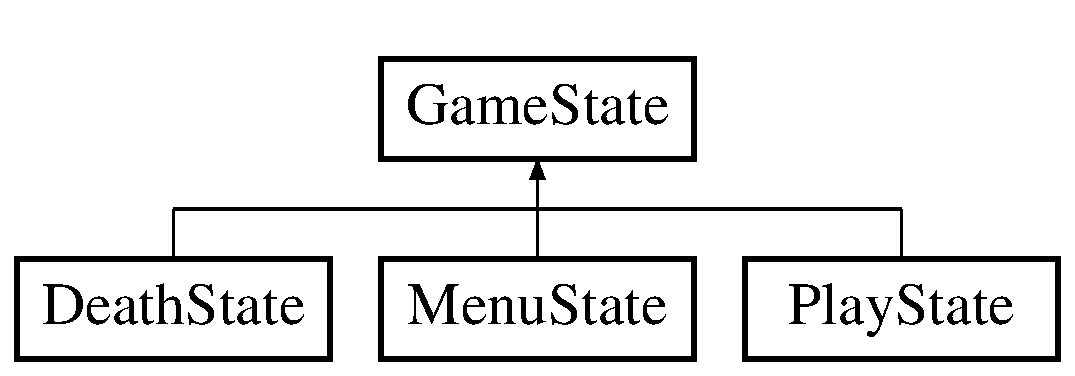
\includegraphics[height=2.000000cm]{class_game_state}
\end{center}
\end{figure}
\subsection*{Public Member Functions}
\begin{DoxyCompactItemize}
\item 
\hypertarget{class_game_state_a6187cf801b77fa905cbe6ad385b4171c}{}virtual void {\bfseries init} ()=0\label{class_game_state_a6187cf801b77fa905cbe6ad385b4171c}

\item 
\hypertarget{class_game_state_a294cb7d91e037226d2223b12f95b1082}{}virtual void {\bfseries cleanup} ()=0\label{class_game_state_a294cb7d91e037226d2223b12f95b1082}

\item 
\hypertarget{class_game_state_a43dce19e114acea697c18e76c4e46893}{}virtual void {\bfseries update} (float const \&delta\+Time)=0\label{class_game_state_a43dce19e114acea697c18e76c4e46893}

\item 
\hypertarget{class_game_state_a35e7c67249e956a975acc180aa359709}{}virtual void {\bfseries handle} (S\+D\+L\+\_\+\+Event event, float delta\+Time)=0\label{class_game_state_a35e7c67249e956a975acc180aa359709}

\end{DoxyCompactItemize}
\subsection*{Public Attributes}
\begin{DoxyCompactItemize}
\item 
\hypertarget{class_game_state_abcdef3f1321523ddec27b9ccbe3787cb}{}std\+::string {\bfseries level} \{\char`\"{}\char`\"{}\}\label{class_game_state_abcdef3f1321523ddec27b9ccbe3787cb}

\item 
\hypertarget{class_game_state_ac03ea6a5b412cd4d2134898453be9049}{}int {\bfseries next\+State} \{\}\label{class_game_state_ac03ea6a5b412cd4d2134898453be9049}

\item 
\hypertarget{class_game_state_a14e5e7cac9f6a8014aa46b457b02f215}{}bool {\bfseries pause} \{false\}\label{class_game_state_a14e5e7cac9f6a8014aa46b457b02f215}

\item 
\hypertarget{class_game_state_a2fbe8294976af31820094bfd26b24f5b}{}int {\bfseries player\+X} \{0\}\label{class_game_state_a2fbe8294976af31820094bfd26b24f5b}

\item 
\hypertarget{class_game_state_a0284357ccdb4a37b613a97a62c44c0ef}{}int {\bfseries player\+Y} \{0\}\label{class_game_state_a0284357ccdb4a37b613a97a62c44c0ef}

\end{DoxyCompactItemize}
\subsection*{Protected Attributes}
\begin{DoxyCompactItemize}
\item 
\hypertarget{class_game_state_a491ae86f9fed2677cb0a3614a9464d11}{}\hyperlink{class_sprite}{Sprite} $\ast$ {\bfseries background}\label{class_game_state_a491ae86f9fed2677cb0a3614a9464d11}

\item 
\hypertarget{class_game_state_afe4de045a38ef13aa48a2c2765eefb12}{}S\+D\+L\+\_\+\+Window $\ast$ {\bfseries window} = nullptr\label{class_game_state_afe4de045a38ef13aa48a2c2765eefb12}

\item 
\hypertarget{class_game_state_a7ed453ab187978a655a8b67c9f4d3672}{}S\+D\+L\+\_\+\+Renderer $\ast$ {\bfseries renderer} = nullptr\label{class_game_state_a7ed453ab187978a655a8b67c9f4d3672}

\item 
\hypertarget{class_game_state_af986003be011f7622bd2b18ba6c2d635}{}std\+::vector$<$ \hyperlink{class_game_object}{Game\+Object} $\ast$ $>$ {\bfseries objects}\label{class_game_state_af986003be011f7622bd2b18ba6c2d635}

\end{DoxyCompactItemize}


The documentation for this class was generated from the following file\+:\begin{DoxyCompactItemize}
\item 
/\+Users/lukas.\+vikstrom/\+Documents/\+T\+D\+P005/\+T\+D\+P005-\/\+Projekt/Game\+State.\+h\end{DoxyCompactItemize}

\hypertarget{class_grass_block}{}\section{Grass\+Block Class Reference}
\label{class_grass_block}\index{Grass\+Block@{Grass\+Block}}
Inheritance diagram for Grass\+Block\+:\begin{figure}[H]
\begin{center}
\leavevmode
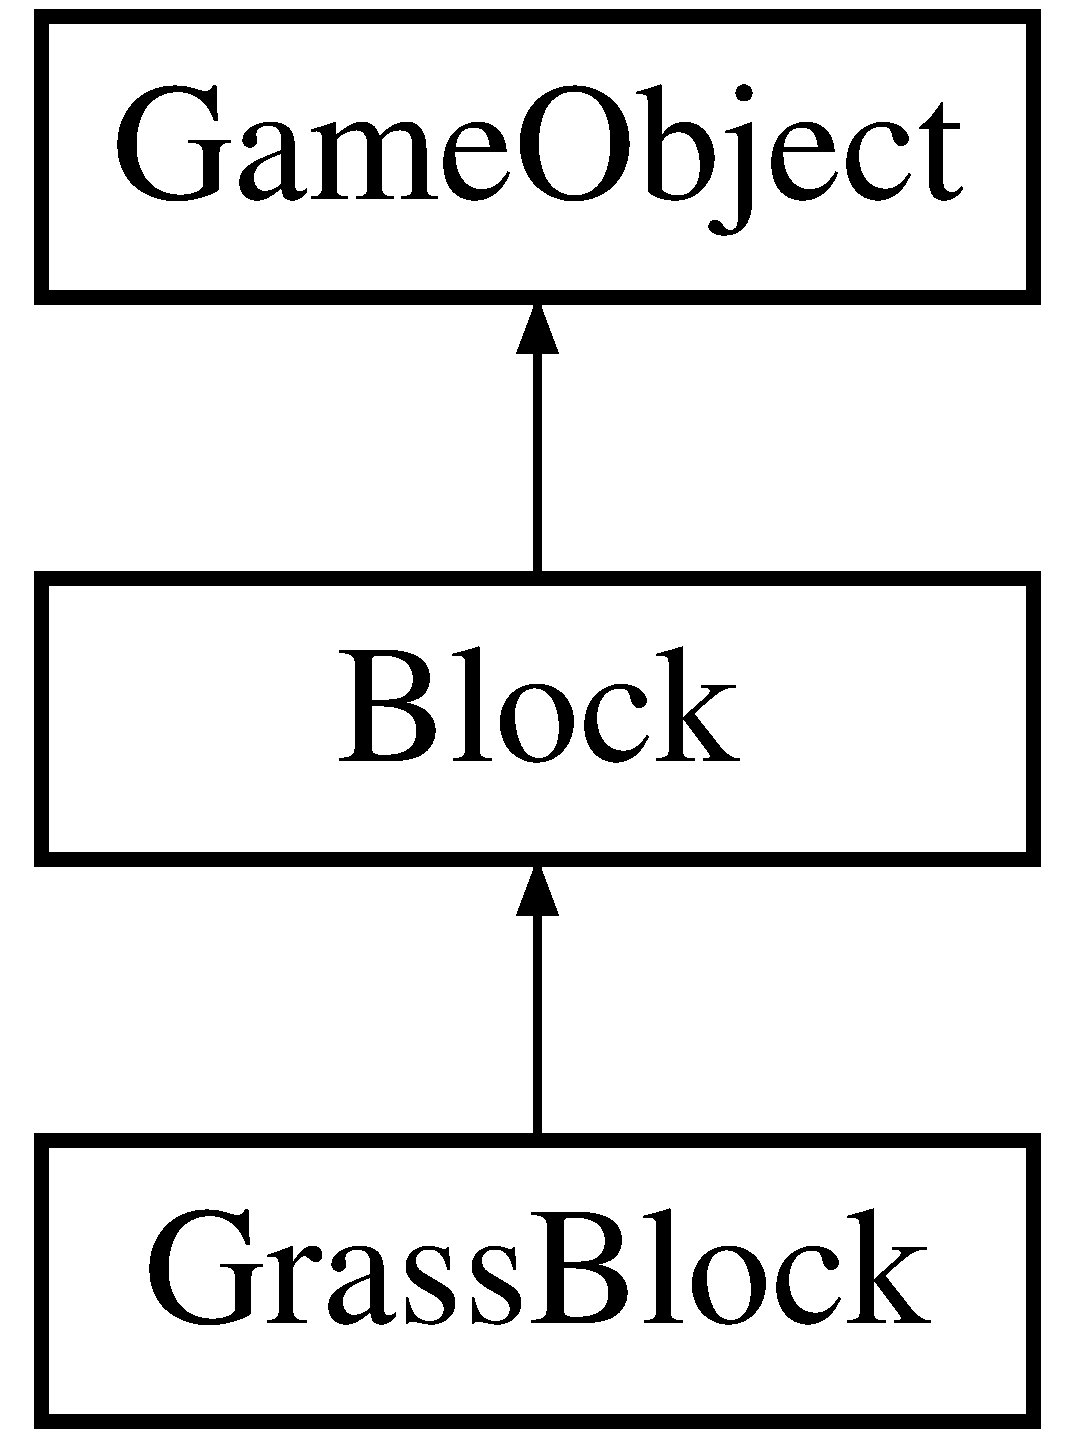
\includegraphics[height=3.000000cm]{class_grass_block}
\end{center}
\end{figure}
\subsection*{Public Member Functions}
\begin{DoxyCompactItemize}
\item 
\hyperlink{class_grass_block_a217d5f4cc197d400811082726a8720cf}{Grass\+Block} (int x\+\_\+pos, int y\+\_\+pos, S\+D\+L\+\_\+\+Renderer $\ast$render)
\begin{DoxyCompactList}\small\item\em Constructor for \hyperlink{class_grass_block}{Grass\+Block}. \end{DoxyCompactList}\end{DoxyCompactItemize}
\subsection*{Additional Inherited Members}


\subsection{Constructor \& Destructor Documentation}
\hypertarget{class_grass_block_a217d5f4cc197d400811082726a8720cf}{}\index{Grass\+Block@{Grass\+Block}!Grass\+Block@{Grass\+Block}}
\index{Grass\+Block@{Grass\+Block}!Grass\+Block@{Grass\+Block}}
\subsubsection[{Grass\+Block(int x\+\_\+pos, int y\+\_\+pos, S\+D\+L\+\_\+\+Renderer $\ast$render)}]{\setlength{\rightskip}{0pt plus 5cm}Grass\+Block\+::\+Grass\+Block (
\begin{DoxyParamCaption}
\item[{int}]{x\+\_\+pos, }
\item[{int}]{y\+\_\+pos, }
\item[{S\+D\+L\+\_\+\+Renderer $\ast$}]{render}
\end{DoxyParamCaption}
)}\label{class_grass_block_a217d5f4cc197d400811082726a8720cf}


Constructor for \hyperlink{class_grass_block}{Grass\+Block}. 


\begin{DoxyParams}{Parameters}
{\em x\+Pos} & x position of block \\
\hline
{\em y\+Pos} & y position of block \\
\hline
{\em render} & renderer to draw to \\
\hline
\end{DoxyParams}


The documentation for this class was generated from the following files\+:\begin{DoxyCompactItemize}
\item 
/\+Users/lukas.\+vikstrom/\+Documents/\+T\+D\+P005/\+T\+D\+P005-\/\+Projekt/Grass\+Block.\+h\item 
/\+Users/lukas.\+vikstrom/\+Documents/\+T\+D\+P005/\+T\+D\+P005-\/\+Projekt/Grass\+Block.\+cc\end{DoxyCompactItemize}

\hypertarget{class_jump_block}{}\section{Jump\+Block Class Reference}
\label{class_jump_block}\index{Jump\+Block@{Jump\+Block}}
Inheritance diagram for Jump\+Block\+:\begin{figure}[H]
\begin{center}
\leavevmode
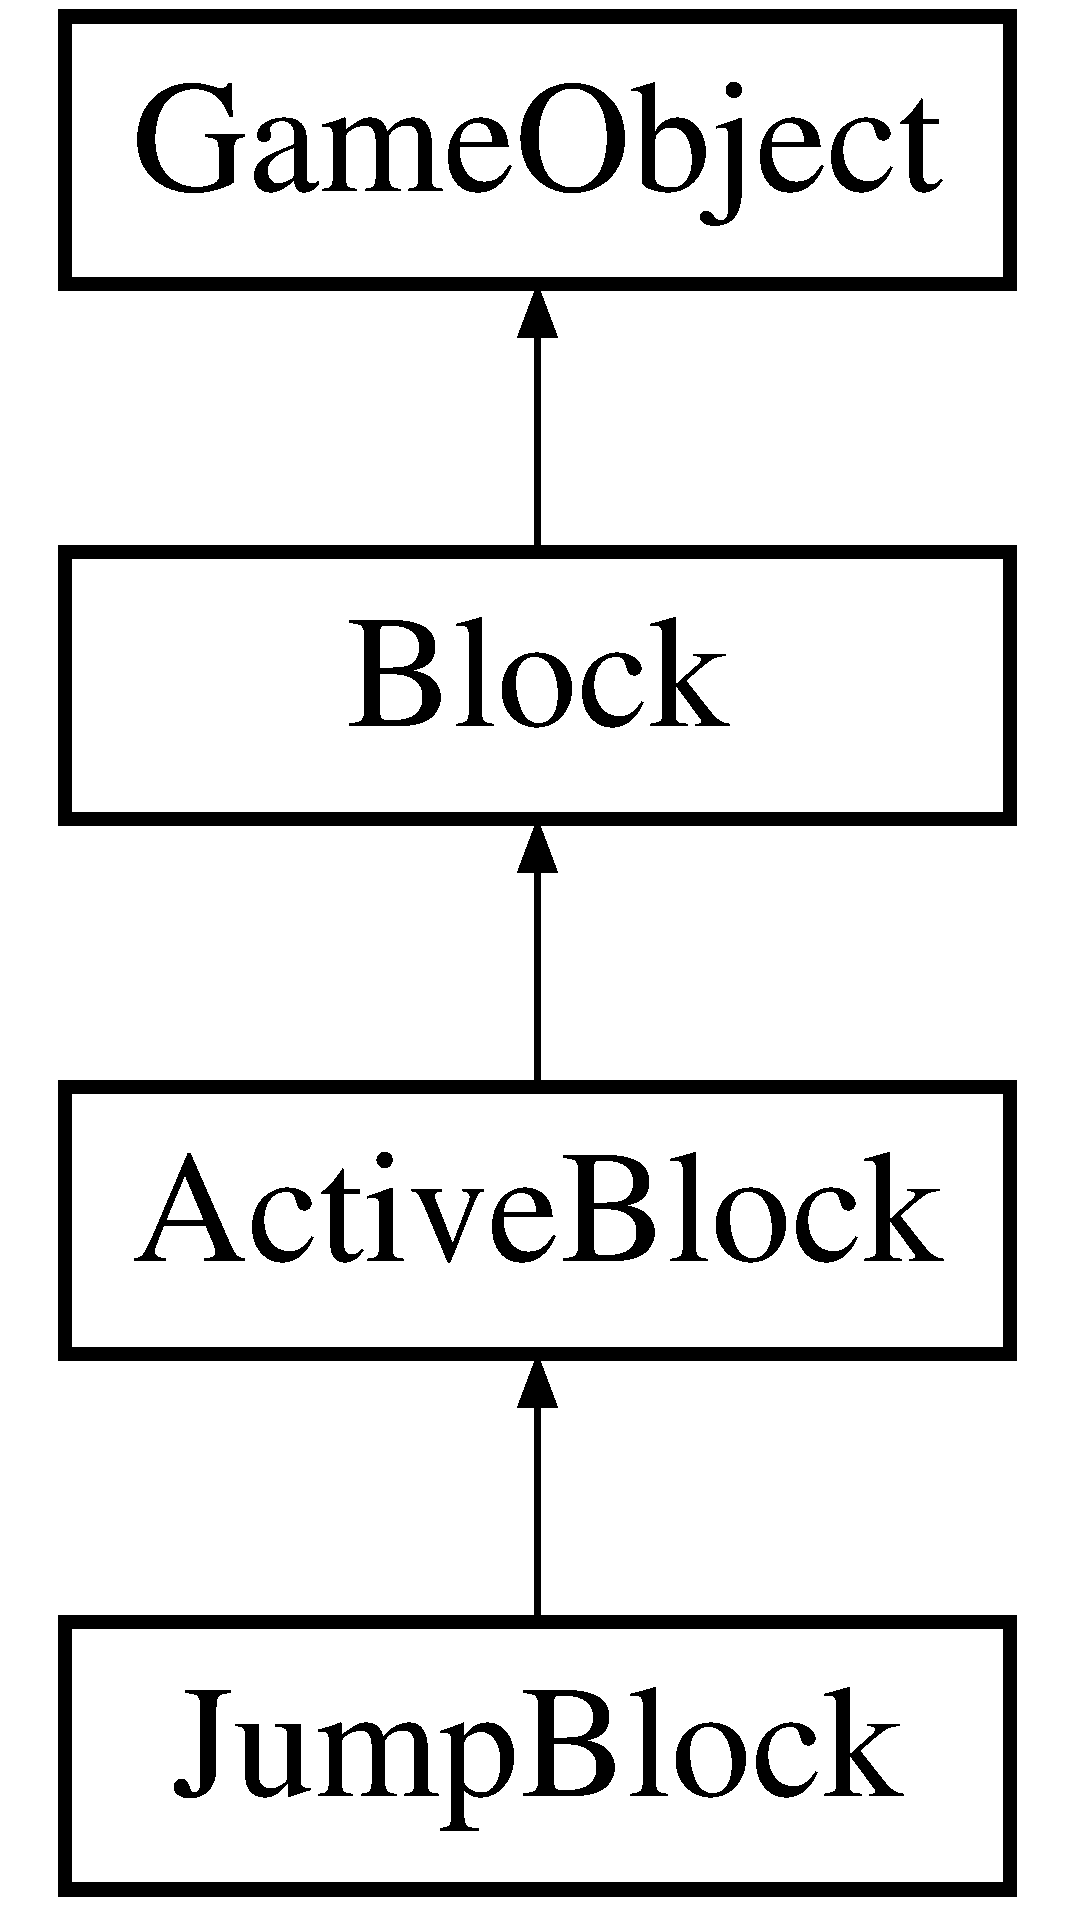
\includegraphics[height=4.000000cm]{class_jump_block}
\end{center}
\end{figure}
\subsection*{Public Member Functions}
\begin{DoxyCompactItemize}
\item 
\hyperlink{class_jump_block_a298527515f74ffcc932b273805110143}{Jump\+Block} (int x\+\_\+pos, int y\+\_\+pos, S\+D\+L\+\_\+\+Renderer $\ast$render)
\begin{DoxyCompactList}\small\item\em Constructor for \hyperlink{class_jump_block}{Jump\+Block}. \end{DoxyCompactList}\item 
\hypertarget{class_jump_block_a1b818f8054c1d0ddee4de45e5b6683d0}{}void {\bfseries activate} ()\label{class_jump_block_a1b818f8054c1d0ddee4de45e5b6683d0}

\end{DoxyCompactItemize}
\subsection*{Additional Inherited Members}


\subsection{Constructor \& Destructor Documentation}
\hypertarget{class_jump_block_a298527515f74ffcc932b273805110143}{}\index{Jump\+Block@{Jump\+Block}!Jump\+Block@{Jump\+Block}}
\index{Jump\+Block@{Jump\+Block}!Jump\+Block@{Jump\+Block}}
\subsubsection[{Jump\+Block(int x\+\_\+pos, int y\+\_\+pos, S\+D\+L\+\_\+\+Renderer $\ast$render)}]{\setlength{\rightskip}{0pt plus 5cm}Jump\+Block\+::\+Jump\+Block (
\begin{DoxyParamCaption}
\item[{int}]{x\+\_\+pos, }
\item[{int}]{y\+\_\+pos, }
\item[{S\+D\+L\+\_\+\+Renderer $\ast$}]{render}
\end{DoxyParamCaption}
)}\label{class_jump_block_a298527515f74ffcc932b273805110143}


Constructor for \hyperlink{class_jump_block}{Jump\+Block}. 


\begin{DoxyParams}{Parameters}
{\em x\+Pos} & x position of block \\
\hline
{\em y\+Pos} & y position of block \\
\hline
{\em render} & renderer to draw to \\
\hline
\end{DoxyParams}


The documentation for this class was generated from the following files\+:\begin{DoxyCompactItemize}
\item 
/\+Users/lukas.\+vikstrom/\+Documents/\+T\+D\+P005/\+T\+D\+P005-\/\+Projekt/Jump\+Block.\+h\item 
/\+Users/lukas.\+vikstrom/\+Documents/\+T\+D\+P005/\+T\+D\+P005-\/\+Projekt/Jump\+Block.\+cc\end{DoxyCompactItemize}

\hypertarget{class_menu_state}{}\section{Menu\+State Class Reference}
\label{class_menu_state}\index{Menu\+State@{Menu\+State}}
Inheritance diagram for Menu\+State\+:\begin{figure}[H]
\begin{center}
\leavevmode
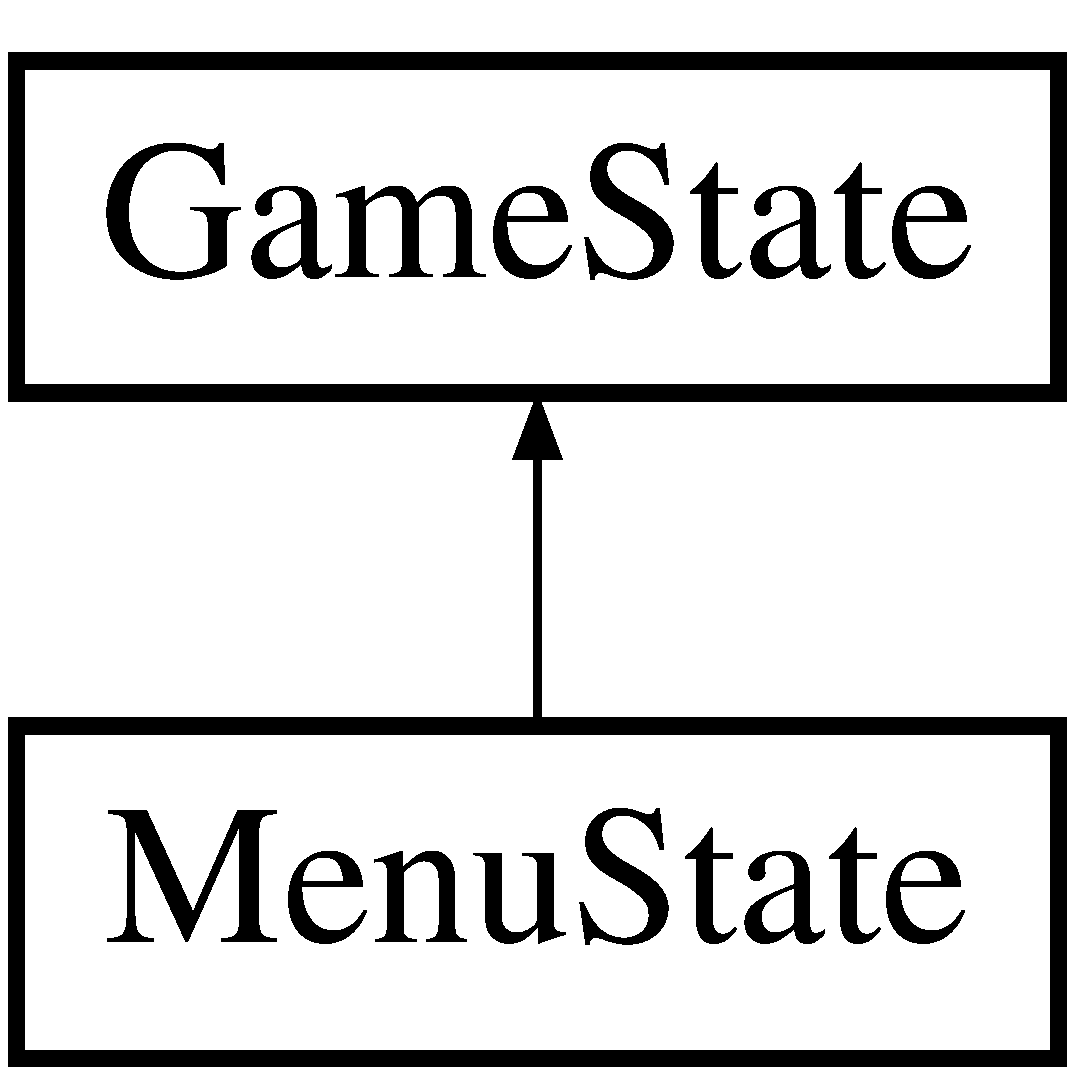
\includegraphics[height=2.000000cm]{class_menu_state}
\end{center}
\end{figure}
\subsection*{Public Member Functions}
\begin{DoxyCompactItemize}
\item 
\hyperlink{class_menu_state_ae4b1263fcc33ec4229c51699b60fbb1e}{Menu\+State} (S\+D\+L\+\_\+\+Window $\ast$win, S\+D\+L\+\_\+\+Renderer $\ast$rend)
\begin{DoxyCompactList}\small\item\em Constructor for \hyperlink{class_menu_state}{Menu\+State}. \end{DoxyCompactList}\item 
void \hyperlink{class_menu_state_a137fc5233d29b03680b35ad1cec3b115}{init} ()
\begin{DoxyCompactList}\small\item\em Initializer for \hyperlink{class_menu_state}{Menu\+State}. \end{DoxyCompactList}\item 
void \hyperlink{class_menu_state_a8996ce14164c5958874633a753a08ed4}{cleanup} ()
\begin{DoxyCompactList}\small\item\em Cleanup for \hyperlink{class_menu_state}{Menu\+State}. \end{DoxyCompactList}\item 
void \hyperlink{class_menu_state_a323c751b4b12bd919738f48733550be1}{update} (float const \&delta\+Time)
\begin{DoxyCompactList}\small\item\em Updator for \hyperlink{class_menu_state}{Menu\+State}. \end{DoxyCompactList}\item 
void \hyperlink{class_menu_state_a5a57d15a22e61a120ca1d26ef4027110}{handle} (S\+D\+L\+\_\+\+Event event, float delta\+Time)
\begin{DoxyCompactList}\small\item\em Event handler for \hyperlink{class_menu_state}{Menu\+State}. \end{DoxyCompactList}\end{DoxyCompactItemize}
\subsection*{Public Attributes}
\begin{DoxyCompactItemize}
\item 
\hypertarget{class_menu_state_a13544c80f87d1fd441ff9fab049d77a7}{}std\+::vector$<$ \hyperlink{class_button}{Button} $\ast$ $>$ {\bfseries menu\+Items}\label{class_menu_state_a13544c80f87d1fd441ff9fab049d77a7}

\end{DoxyCompactItemize}
\subsection*{Additional Inherited Members}


\subsection{Constructor \& Destructor Documentation}
\hypertarget{class_menu_state_ae4b1263fcc33ec4229c51699b60fbb1e}{}\index{Menu\+State@{Menu\+State}!Menu\+State@{Menu\+State}}
\index{Menu\+State@{Menu\+State}!Menu\+State@{Menu\+State}}
\subsubsection[{Menu\+State(\+S\+D\+L\+\_\+\+Window $\ast$win, S\+D\+L\+\_\+\+Renderer $\ast$rend)}]{\setlength{\rightskip}{0pt plus 5cm}Menu\+State\+::\+Menu\+State (
\begin{DoxyParamCaption}
\item[{S\+D\+L\+\_\+\+Window $\ast$}]{win, }
\item[{S\+D\+L\+\_\+\+Renderer $\ast$}]{rend}
\end{DoxyParamCaption}
)}\label{class_menu_state_ae4b1263fcc33ec4229c51699b60fbb1e}


Constructor for \hyperlink{class_menu_state}{Menu\+State}. 


\begin{DoxyParams}{Parameters}
{\em win} & window to draw to \\
\hline
{\em rend} & renderer to draw to \\
\hline
\end{DoxyParams}


\subsection{Member Function Documentation}
\hypertarget{class_menu_state_a8996ce14164c5958874633a753a08ed4}{}\index{Menu\+State@{Menu\+State}!cleanup@{cleanup}}
\index{cleanup@{cleanup}!Menu\+State@{Menu\+State}}
\subsubsection[{cleanup()}]{\setlength{\rightskip}{0pt plus 5cm}void Menu\+State\+::cleanup (
\begin{DoxyParamCaption}
{}
\end{DoxyParamCaption}
)\hspace{0.3cm}{\ttfamily [virtual]}}\label{class_menu_state_a8996ce14164c5958874633a753a08ed4}


Cleanup for \hyperlink{class_menu_state}{Menu\+State}. 

Deletes all buttons and the background. 

Implements \hyperlink{class_game_state}{Game\+State}.

\hypertarget{class_menu_state_a5a57d15a22e61a120ca1d26ef4027110}{}\index{Menu\+State@{Menu\+State}!handle@{handle}}
\index{handle@{handle}!Menu\+State@{Menu\+State}}
\subsubsection[{handle(\+S\+D\+L\+\_\+\+Event event, float delta\+Time)}]{\setlength{\rightskip}{0pt plus 5cm}void Menu\+State\+::handle (
\begin{DoxyParamCaption}
\item[{S\+D\+L\+\_\+\+Event}]{event, }
\item[{float}]{delta\+Time}
\end{DoxyParamCaption}
)\hspace{0.3cm}{\ttfamily [virtual]}}\label{class_menu_state_a5a57d15a22e61a120ca1d26ef4027110}


Event handler for \hyperlink{class_menu_state}{Menu\+State}. 

Handles mouse clicks and checks if the click occurred on a button and then loads the appropriate level. 

Implements \hyperlink{class_game_state}{Game\+State}.

\hypertarget{class_menu_state_a137fc5233d29b03680b35ad1cec3b115}{}\index{Menu\+State@{Menu\+State}!init@{init}}
\index{init@{init}!Menu\+State@{Menu\+State}}
\subsubsection[{init()}]{\setlength{\rightskip}{0pt plus 5cm}void Menu\+State\+::init (
\begin{DoxyParamCaption}
{}
\end{DoxyParamCaption}
)\hspace{0.3cm}{\ttfamily [virtual]}}\label{class_menu_state_a137fc5233d29b03680b35ad1cec3b115}


Initializer for \hyperlink{class_menu_state}{Menu\+State}. 

Loads image to menu background and adds buttons for the different levels. 

Implements \hyperlink{class_game_state}{Game\+State}.

\hypertarget{class_menu_state_a323c751b4b12bd919738f48733550be1}{}\index{Menu\+State@{Menu\+State}!update@{update}}
\index{update@{update}!Menu\+State@{Menu\+State}}
\subsubsection[{update(float const \&delta\+Time)}]{\setlength{\rightskip}{0pt plus 5cm}void Menu\+State\+::update (
\begin{DoxyParamCaption}
\item[{float const \&}]{delta\+Time}
\end{DoxyParamCaption}
)\hspace{0.3cm}{\ttfamily [virtual]}}\label{class_menu_state_a323c751b4b12bd919738f48733550be1}


Updator for \hyperlink{class_menu_state}{Menu\+State}. 

Clears the screen and draws the background and buttons. 

Implements \hyperlink{class_game_state}{Game\+State}.



The documentation for this class was generated from the following files\+:\begin{DoxyCompactItemize}
\item 
/\+Users/lukas.\+vikstrom/\+Documents/\+T\+D\+P005/\+T\+D\+P005-\/\+Projekt/Menu\+State.\+h\item 
/\+Users/lukas.\+vikstrom/\+Documents/\+T\+D\+P005/\+T\+D\+P005-\/\+Projekt/Menu\+State.\+cc\end{DoxyCompactItemize}

\hypertarget{class_mr_rabbit}{}\section{Mr\+Rabbit Class Reference}
\label{class_mr_rabbit}\index{Mr\+Rabbit@{Mr\+Rabbit}}
Inheritance diagram for Mr\+Rabbit\+:\begin{figure}[H]
\begin{center}
\leavevmode
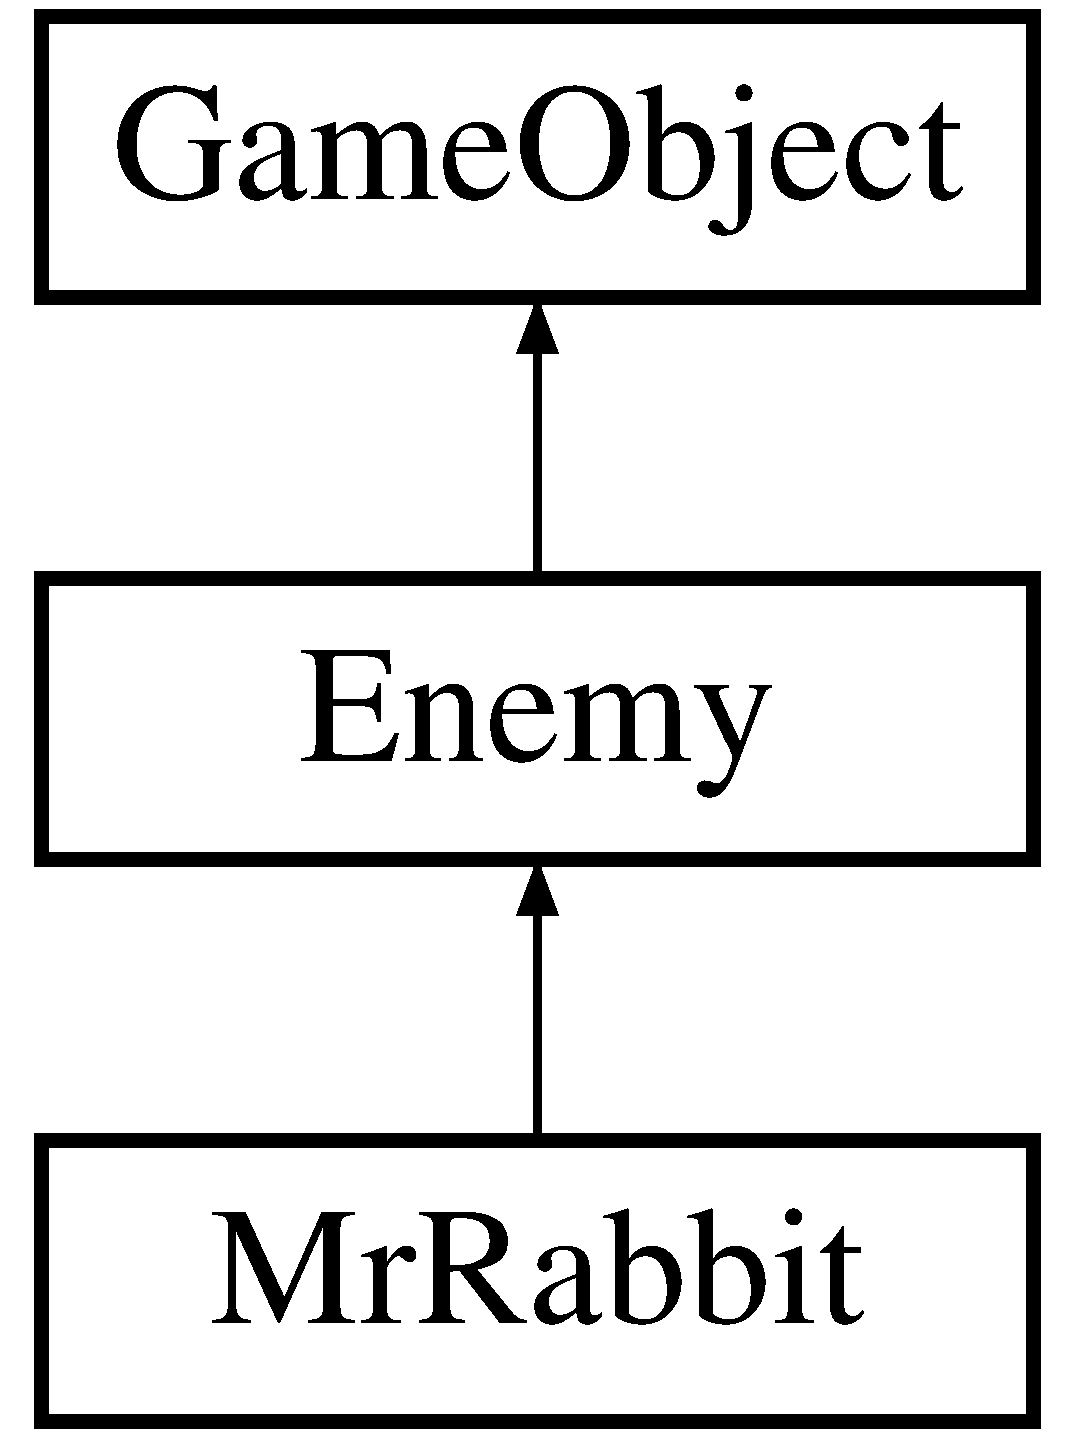
\includegraphics[height=3.000000cm]{class_mr_rabbit}
\end{center}
\end{figure}
\subsection*{Public Member Functions}
\begin{DoxyCompactItemize}
\item 
\hyperlink{class_mr_rabbit_a9b8c7154199faef4d81134cf231bd53d}{Mr\+Rabbit} (int x\+\_\+pos, int y\+\_\+pos, S\+D\+L\+\_\+\+Renderer $\ast$render, \hyperlink{class_player}{Player} $\ast$player\+\_\+ptr)
\begin{DoxyCompactList}\small\item\em Constructor for \hyperlink{class_mr_rabbit}{Mr\+Rabbit}. \end{DoxyCompactList}\item 
void \hyperlink{class_mr_rabbit_ac5a5229bd3b1b8be9b7edd0f86fa754d}{update} (float const \&delta\+Time)
\begin{DoxyCompactList}\small\item\em Updator for \hyperlink{class_mr_rabbit}{Mr\+Rabbit}. \end{DoxyCompactList}\item 
void \hyperlink{class_mr_rabbit_a68b8b4781ddb1a449b52425a11d035bf}{decide\+Action} ()
\begin{DoxyCompactList}\small\item\em Decides the next action for mr. rabbit. \end{DoxyCompactList}\item 
void \hyperlink{class_mr_rabbit_a117b3bd7ec5019a5bdaf3de39f473397}{create\+Object} (std\+::vector$<$ \hyperlink{class_game_object}{Game\+Object} $\ast$ $>$ \&map\+\_\+objects)
\begin{DoxyCompactList}\small\item\em Creates the mr. rabbit projectile. \end{DoxyCompactList}\item 
void \hyperlink{class_mr_rabbit_a18dbce185702a664bd85e4c4689df415}{will\+Collide} (std\+::vector$<$ \hyperlink{class_game_object}{Game\+Object} $\ast$ $>$ const \&objects)
\begin{DoxyCompactList}\small\item\em Checks for collision with every object on the screen and handles it if collision has occurred. \end{DoxyCompactList}\end{DoxyCompactItemize}
\subsection*{Additional Inherited Members}


\subsection{Constructor \& Destructor Documentation}
\hypertarget{class_mr_rabbit_a9b8c7154199faef4d81134cf231bd53d}{}\index{Mr\+Rabbit@{Mr\+Rabbit}!Mr\+Rabbit@{Mr\+Rabbit}}
\index{Mr\+Rabbit@{Mr\+Rabbit}!Mr\+Rabbit@{Mr\+Rabbit}}
\subsubsection[{Mr\+Rabbit(int x\+\_\+pos, int y\+\_\+pos, S\+D\+L\+\_\+\+Renderer $\ast$render, Player $\ast$player\+\_\+ptr)}]{\setlength{\rightskip}{0pt plus 5cm}Mr\+Rabbit\+::\+Mr\+Rabbit (
\begin{DoxyParamCaption}
\item[{int}]{x\+\_\+pos, }
\item[{int}]{y\+\_\+pos, }
\item[{S\+D\+L\+\_\+\+Renderer $\ast$}]{render, }
\item[{{\bf Player} $\ast$}]{player\+\_\+ptr}
\end{DoxyParamCaption}
)}\label{class_mr_rabbit_a9b8c7154199faef4d81134cf231bd53d}


Constructor for \hyperlink{class_mr_rabbit}{Mr\+Rabbit}. 


\begin{DoxyParams}{Parameters}
{\em x\+Pos} & x position of mr. rabbit \\
\hline
{\em y\+Pos} & y position of mr. rabbit \\
\hline
{\em render} & renderer to draw to \\
\hline
{\em player\+\_\+ptr} & pointer to active player \\
\hline
\end{DoxyParams}


\subsection{Member Function Documentation}
\hypertarget{class_mr_rabbit_a117b3bd7ec5019a5bdaf3de39f473397}{}\index{Mr\+Rabbit@{Mr\+Rabbit}!create\+Object@{create\+Object}}
\index{create\+Object@{create\+Object}!Mr\+Rabbit@{Mr\+Rabbit}}
\subsubsection[{create\+Object(std\+::vector$<$ Game\+Object $\ast$ $>$ \&map\+\_\+objects)}]{\setlength{\rightskip}{0pt plus 5cm}void Mr\+Rabbit\+::create\+Object (
\begin{DoxyParamCaption}
\item[{std\+::vector$<$ {\bf Game\+Object} $\ast$ $>$ \&}]{map\+\_\+objects}
\end{DoxyParamCaption}
)\hspace{0.3cm}{\ttfamily [virtual]}}\label{class_mr_rabbit_a117b3bd7ec5019a5bdaf3de39f473397}


Creates the mr. rabbit projectile. 

Creates mr. rabbits projectile if he is able to shoot and then resets the variable related to shooting 

Reimplemented from \hyperlink{class_game_object}{Game\+Object}.

\hypertarget{class_mr_rabbit_a68b8b4781ddb1a449b52425a11d035bf}{}\index{Mr\+Rabbit@{Mr\+Rabbit}!decide\+Action@{decide\+Action}}
\index{decide\+Action@{decide\+Action}!Mr\+Rabbit@{Mr\+Rabbit}}
\subsubsection[{decide\+Action()}]{\setlength{\rightskip}{0pt plus 5cm}void Mr\+Rabbit\+::decide\+Action (
\begin{DoxyParamCaption}
{}
\end{DoxyParamCaption}
)\hspace{0.3cm}{\ttfamily [virtual]}}\label{class_mr_rabbit_a68b8b4781ddb1a449b52425a11d035bf}


Decides the next action for mr. rabbit. 

Shoots next update and changes to correct direction if player is within a certain x or y distance. Moves right or left depending in the time since last movement. 

Implements \hyperlink{class_enemy}{Enemy}.

\hypertarget{class_mr_rabbit_ac5a5229bd3b1b8be9b7edd0f86fa754d}{}\index{Mr\+Rabbit@{Mr\+Rabbit}!update@{update}}
\index{update@{update}!Mr\+Rabbit@{Mr\+Rabbit}}
\subsubsection[{update(float const \&delta\+Time)}]{\setlength{\rightskip}{0pt plus 5cm}void Mr\+Rabbit\+::update (
\begin{DoxyParamCaption}
\item[{float const \&}]{delta\+Time}
\end{DoxyParamCaption}
)\hspace{0.3cm}{\ttfamily [virtual]}}\label{class_mr_rabbit_ac5a5229bd3b1b8be9b7edd0f86fa754d}


Updator for \hyperlink{class_mr_rabbit}{Mr\+Rabbit}. 

Resets the bool that states if a collision has occurred this update. Decides the next action to take. Updates the time variable used to make decisions and the time since last shot variable. Updates x position of the object. Updates y position of the object according to gravity calculations. 

Implements \hyperlink{class_game_object}{Game\+Object}.

\hypertarget{class_mr_rabbit_a18dbce185702a664bd85e4c4689df415}{}\index{Mr\+Rabbit@{Mr\+Rabbit}!will\+Collide@{will\+Collide}}
\index{will\+Collide@{will\+Collide}!Mr\+Rabbit@{Mr\+Rabbit}}
\subsubsection[{will\+Collide(std\+::vector$<$ Game\+Object $\ast$ $>$ const \&objects)}]{\setlength{\rightskip}{0pt plus 5cm}void Mr\+Rabbit\+::will\+Collide (
\begin{DoxyParamCaption}
\item[{std\+::vector$<$ {\bf Game\+Object} $\ast$ $>$ const \&}]{objects}
\end{DoxyParamCaption}
)\hspace{0.3cm}{\ttfamily [virtual]}}\label{class_mr_rabbit_a18dbce185702a664bd85e4c4689df415}


Checks for collision with every object on the screen and handles it if collision has occurred. 

Creates a vector that will contain the object and the type of the object it collides with. Creates a vector with the resulting collision direction of the object it collides with. Loops through all objects on screen and checks for collision. Calls handle\+Collision() with the previously mentioned vector containing the object and its type. 

Implements \hyperlink{class_game_object}{Game\+Object}.



The documentation for this class was generated from the following files\+:\begin{DoxyCompactItemize}
\item 
/\+Users/lukas.\+vikstrom/\+Documents/\+T\+D\+P005/\+T\+D\+P005-\/\+Projekt/Mr\+Rabbit.\+h\item 
/\+Users/lukas.\+vikstrom/\+Documents/\+T\+D\+P005/\+T\+D\+P005-\/\+Projekt/Mr\+Rabbit.\+cc\end{DoxyCompactItemize}

\hypertarget{class_mr_rabbit_projectile}{}\section{Mr\+Rabbit\+Projectile Class Reference}
\label{class_mr_rabbit_projectile}\index{Mr\+Rabbit\+Projectile@{Mr\+Rabbit\+Projectile}}
Inheritance diagram for Mr\+Rabbit\+Projectile\+:\begin{figure}[H]
\begin{center}
\leavevmode
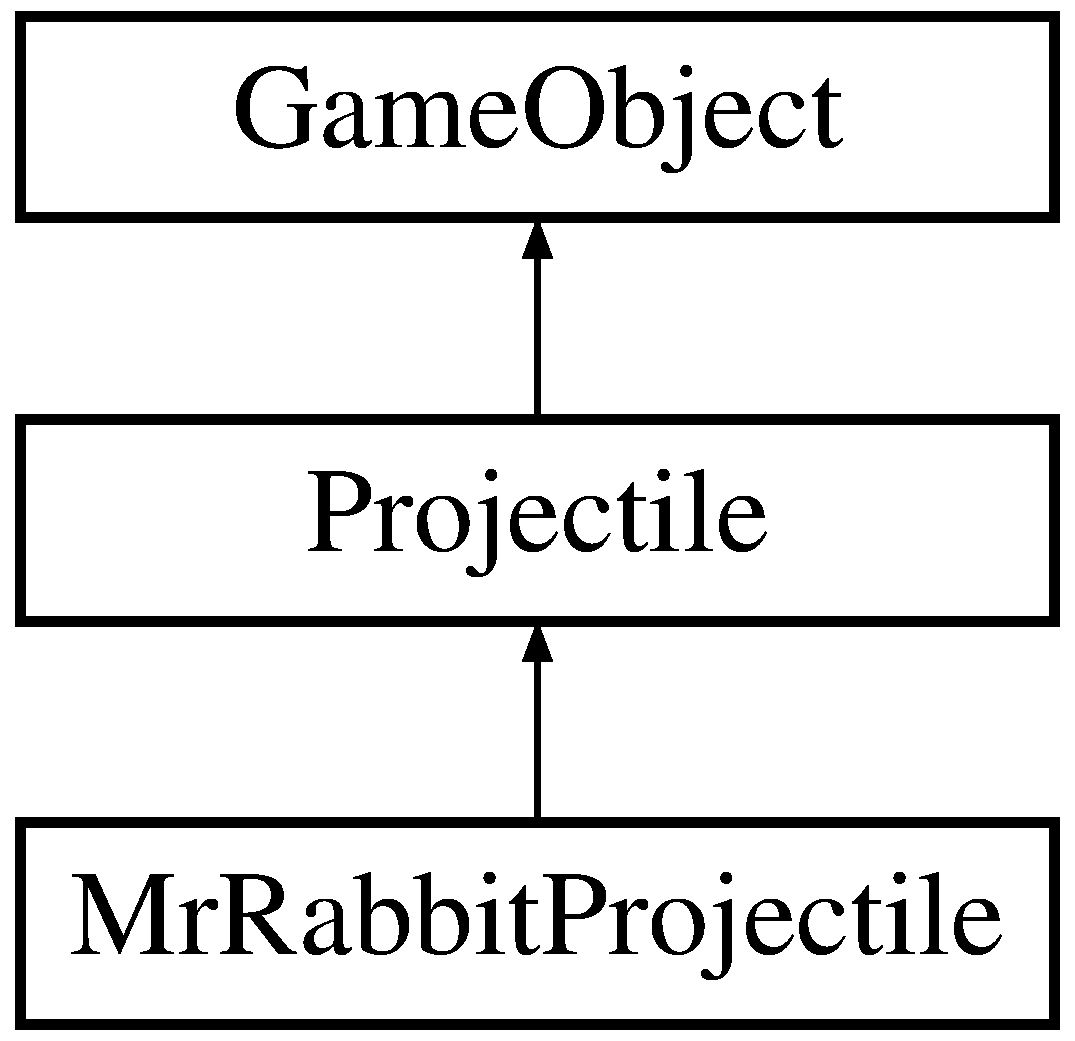
\includegraphics[height=3.000000cm]{class_mr_rabbit_projectile}
\end{center}
\end{figure}
\subsection*{Public Member Functions}
\begin{DoxyCompactItemize}
\item 
\hypertarget{class_mr_rabbit_projectile_ac56afebb86e536ea16434b927c8a2662}{}{\bfseries Mr\+Rabbit\+Projectile} (int x, int y, int dir, S\+D\+L\+\_\+\+Renderer $\ast$render, \hyperlink{class_game_object}{Game\+Object} $\ast$creator\+\_\+ptr)\label{class_mr_rabbit_projectile_ac56afebb86e536ea16434b927c8a2662}

\end{DoxyCompactItemize}
\subsection*{Additional Inherited Members}


The documentation for this class was generated from the following files\+:\begin{DoxyCompactItemize}
\item 
/\+Users/lukas.\+vikstrom/\+Documents/\+T\+D\+P005/\+T\+D\+P005-\/\+Projekt/Mr\+Rabbit\+Projectile.\+h\item 
/\+Users/lukas.\+vikstrom/\+Documents/\+T\+D\+P005/\+T\+D\+P005-\/\+Projekt/Mr\+Rabbit\+Projectile.\+cc\end{DoxyCompactItemize}

\hypertarget{class_player}{}\section{Player Class Reference}
\label{class_player}\index{Player@{Player}}
Inheritance diagram for Player\+:\begin{figure}[H]
\begin{center}
\leavevmode
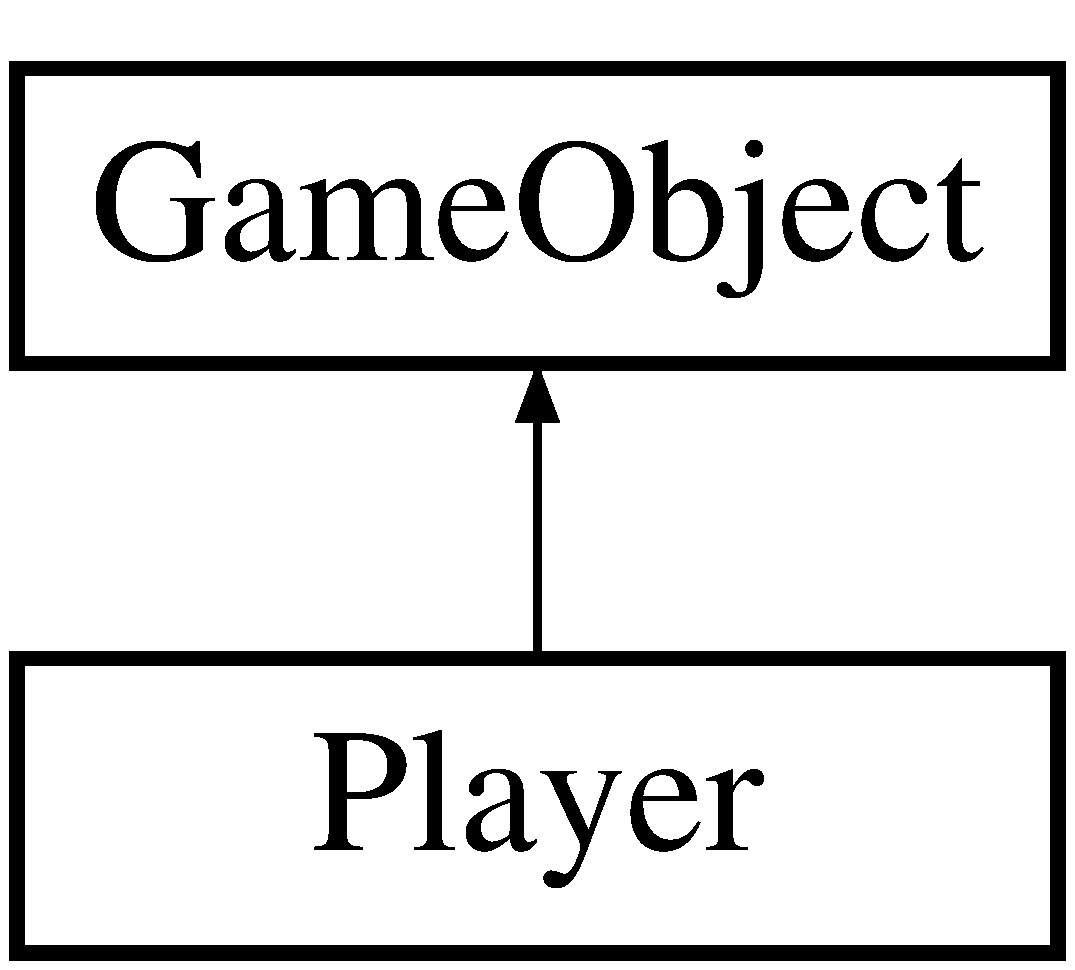
\includegraphics[height=2.000000cm]{class_player}
\end{center}
\end{figure}
\subsection*{Public Member Functions}
\begin{DoxyCompactItemize}
\item 
\hyperlink{class_player_a38a728782dce5a00c9afc53f35541ba1}{Player} (int x\+\_\+pos, int y\+\_\+pos, S\+D\+L\+\_\+\+Renderer $\ast$render)
\begin{DoxyCompactList}\small\item\em Constructor for \hyperlink{class_player}{Player}. \end{DoxyCompactList}\item 
void \hyperlink{class_player_af4975b4e4ee42b8cce9e5d4c58e0c3d2}{handle} (S\+D\+L\+\_\+\+Event event, float delta\+Time)
\begin{DoxyCompactList}\small\item\em Event handler for \hyperlink{class_player}{Player}. \end{DoxyCompactList}\item 
void \hyperlink{class_player_a731b1520afe3330d9fadd7a96512f935}{will\+Collide} (std\+::vector$<$ \hyperlink{class_game_object}{Game\+Object} $\ast$ $>$ const \&objects)
\begin{DoxyCompactList}\small\item\em Checks for collision with every object on the screen and handles it if collision has occurred. \end{DoxyCompactList}\item 
void \hyperlink{class_player_a89be03c84da08f8a10158da5144a484f}{create\+Object} (std\+::vector$<$ \hyperlink{class_game_object}{Game\+Object} $\ast$ $>$ \&map\+\_\+objects)
\begin{DoxyCompactList}\small\item\em Creates the players projectile. \end{DoxyCompactList}\item 
void \hyperlink{class_player_a5c4e438772f28154277cf326272d8a86}{update} (float const \&delta\+Time)
\begin{DoxyCompactList}\small\item\em Updator for \hyperlink{class_player}{Player}. \end{DoxyCompactList}\item 
\hypertarget{class_player_a3a3cb6f5b734b7a64ee78b121e1e4797}{}std\+::string {\bfseries get\+Next\+Sub\+Level} ()\label{class_player_a3a3cb6f5b734b7a64ee78b121e1e4797}

\item 
bool \hyperlink{class_player_a175d4becaf0de5ceaa7c1b4c1f8d697a}{should\+Change\+Sub\+Level} ()
\begin{DoxyCompactList}\small\item\em Determines if it should (can) change sublevel. \end{DoxyCompactList}\end{DoxyCompactItemize}
\subsection*{Public Attributes}
\begin{DoxyCompactItemize}
\item 
\hypertarget{class_player_a545c9c9c29c204c505b3773b13a08617}{}int {\bfseries jump\+Power} \{1\}\label{class_player_a545c9c9c29c204c505b3773b13a08617}

\end{DoxyCompactItemize}
\subsection*{Additional Inherited Members}


\subsection{Constructor \& Destructor Documentation}
\hypertarget{class_player_a38a728782dce5a00c9afc53f35541ba1}{}\index{Player@{Player}!Player@{Player}}
\index{Player@{Player}!Player@{Player}}
\subsubsection[{Player(int x\+\_\+pos, int y\+\_\+pos, S\+D\+L\+\_\+\+Renderer $\ast$render)}]{\setlength{\rightskip}{0pt plus 5cm}Player\+::\+Player (
\begin{DoxyParamCaption}
\item[{int}]{x\+\_\+pos, }
\item[{int}]{y\+\_\+pos, }
\item[{S\+D\+L\+\_\+\+Renderer $\ast$}]{render}
\end{DoxyParamCaption}
)}\label{class_player_a38a728782dce5a00c9afc53f35541ba1}


Constructor for \hyperlink{class_player}{Player}. 


\begin{DoxyParams}{Parameters}
{\em x\+Pos} & x position of player \\
\hline
{\em y\+Pos} & y position of player \\
\hline
{\em render} & renderer to draw to \\
\hline
\end{DoxyParams}


\subsection{Member Function Documentation}
\hypertarget{class_player_a89be03c84da08f8a10158da5144a484f}{}\index{Player@{Player}!create\+Object@{create\+Object}}
\index{create\+Object@{create\+Object}!Player@{Player}}
\subsubsection[{create\+Object(std\+::vector$<$ Game\+Object $\ast$ $>$ \&map\+\_\+objects)}]{\setlength{\rightskip}{0pt plus 5cm}void Player\+::create\+Object (
\begin{DoxyParamCaption}
\item[{std\+::vector$<$ {\bf Game\+Object} $\ast$ $>$ \&}]{map\+\_\+objects}
\end{DoxyParamCaption}
)\hspace{0.3cm}{\ttfamily [virtual]}}\label{class_player_a89be03c84da08f8a10158da5144a484f}


Creates the players projectile. 

Creates player projectile if he is able to shoot and then resets the variable related to shooting 

Reimplemented from \hyperlink{class_game_object}{Game\+Object}.

\hypertarget{class_player_af4975b4e4ee42b8cce9e5d4c58e0c3d2}{}\index{Player@{Player}!handle@{handle}}
\index{handle@{handle}!Player@{Player}}
\subsubsection[{handle(\+S\+D\+L\+\_\+\+Event event, float delta\+Time)}]{\setlength{\rightskip}{0pt plus 5cm}void Player\+::handle (
\begin{DoxyParamCaption}
\item[{S\+D\+L\+\_\+\+Event}]{event, }
\item[{float}]{delta\+Time}
\end{DoxyParamCaption}
)}\label{class_player_af4975b4e4ee42b8cce9e5d4c58e0c3d2}


Event handler for \hyperlink{class_player}{Player}. 

Resets x velocity to zero when movement keys are no longer pressed. Resets boolean that states if projectile can be shot next update when spacebar is no longer pressed. Calls appropriate move or jump functions if movement keys are presesed. Calls shoot function if space bar is pressed. Kills player if R is pressed. \hypertarget{class_player_a175d4becaf0de5ceaa7c1b4c1f8d697a}{}\index{Player@{Player}!should\+Change\+Sub\+Level@{should\+Change\+Sub\+Level}}
\index{should\+Change\+Sub\+Level@{should\+Change\+Sub\+Level}!Player@{Player}}
\subsubsection[{should\+Change\+Sub\+Level()}]{\setlength{\rightskip}{0pt plus 5cm}bool Player\+::should\+Change\+Sub\+Level (
\begin{DoxyParamCaption}
{}
\end{DoxyParamCaption}
)}\label{class_player_a175d4becaf0de5ceaa7c1b4c1f8d697a}


Determines if it should (can) change sublevel. 

\begin{DoxyReturn}{Returns}
if the next sublevel isn\textquotesingle{}t an empty string it returns true. 
\end{DoxyReturn}
\hypertarget{class_player_a5c4e438772f28154277cf326272d8a86}{}\index{Player@{Player}!update@{update}}
\index{update@{update}!Player@{Player}}
\subsubsection[{update(float const \&delta\+Time)}]{\setlength{\rightskip}{0pt plus 5cm}void Player\+::update (
\begin{DoxyParamCaption}
\item[{float const \&}]{delta\+Time}
\end{DoxyParamCaption}
)\hspace{0.3cm}{\ttfamily [virtual]}}\label{class_player_a5c4e438772f28154277cf326272d8a86}


Updator for \hyperlink{class_player}{Player}. 

Resets the bool that states if a collision has occurred this update. Updates the time since last shot. Updates x position of the object. Updates y position of the object according to gravity calculations. 

Implements \hyperlink{class_game_object}{Game\+Object}.

\hypertarget{class_player_a731b1520afe3330d9fadd7a96512f935}{}\index{Player@{Player}!will\+Collide@{will\+Collide}}
\index{will\+Collide@{will\+Collide}!Player@{Player}}
\subsubsection[{will\+Collide(std\+::vector$<$ Game\+Object $\ast$ $>$ const \&objects)}]{\setlength{\rightskip}{0pt plus 5cm}void Player\+::will\+Collide (
\begin{DoxyParamCaption}
\item[{std\+::vector$<$ {\bf Game\+Object} $\ast$ $>$ const \&}]{objects}
\end{DoxyParamCaption}
)\hspace{0.3cm}{\ttfamily [virtual]}}\label{class_player_a731b1520afe3330d9fadd7a96512f935}


Checks for collision with every object on the screen and handles it if collision has occurred. 

Creates a vector that will contain the object and the type of the object it collides with. Creates a vector with the resulting collision direction of the object it collides with. Loops through all objects on screen and checks for collision. Calls handle\+Collision() with the previously mentioned vector containing the object and its type. 

Implements \hyperlink{class_game_object}{Game\+Object}.



The documentation for this class was generated from the following files\+:\begin{DoxyCompactItemize}
\item 
/\+Users/lukas.\+vikstrom/\+Documents/\+T\+D\+P005/\+T\+D\+P005-\/\+Projekt/Player.\+h\item 
/\+Users/lukas.\+vikstrom/\+Documents/\+T\+D\+P005/\+T\+D\+P005-\/\+Projekt/Player.\+cc\end{DoxyCompactItemize}

\hypertarget{class_player_projectile}{}\section{Player\+Projectile Class Reference}
\label{class_player_projectile}\index{Player\+Projectile@{Player\+Projectile}}
Inheritance diagram for Player\+Projectile\+:\begin{figure}[H]
\begin{center}
\leavevmode
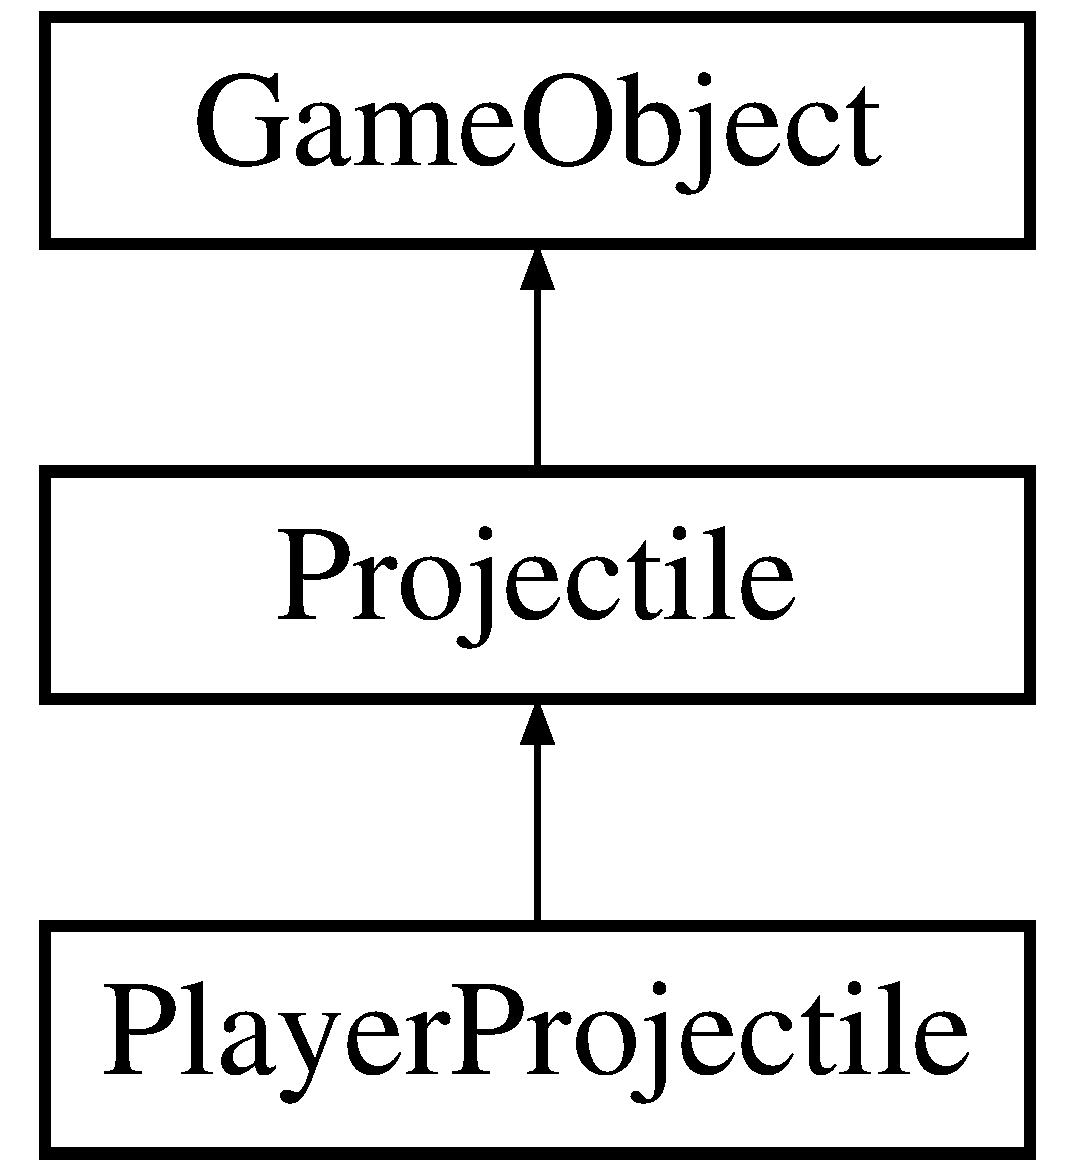
\includegraphics[height=3.000000cm]{class_player_projectile}
\end{center}
\end{figure}
\subsection*{Public Member Functions}
\begin{DoxyCompactItemize}
\item 
\hyperlink{class_player_projectile_a500160841d1cd4fd7085448cb8766989}{Player\+Projectile} (int x, int y, int dir, S\+D\+L\+\_\+\+Renderer $\ast$render, \hyperlink{class_game_object}{Game\+Object} $\ast$creator\+\_\+ptr)
\begin{DoxyCompactList}\small\item\em Constructor for \hyperlink{class_player_projectile}{Player\+Projectile}. \end{DoxyCompactList}\end{DoxyCompactItemize}
\subsection*{Additional Inherited Members}


\subsection{Constructor \& Destructor Documentation}
\hypertarget{class_player_projectile_a500160841d1cd4fd7085448cb8766989}{}\index{Player\+Projectile@{Player\+Projectile}!Player\+Projectile@{Player\+Projectile}}
\index{Player\+Projectile@{Player\+Projectile}!Player\+Projectile@{Player\+Projectile}}
\subsubsection[{Player\+Projectile(int x, int y, int dir, S\+D\+L\+\_\+\+Renderer $\ast$render, Game\+Object $\ast$creator\+\_\+ptr)}]{\setlength{\rightskip}{0pt plus 5cm}Player\+Projectile\+::\+Player\+Projectile (
\begin{DoxyParamCaption}
\item[{int}]{x, }
\item[{int}]{y, }
\item[{int}]{dir, }
\item[{S\+D\+L\+\_\+\+Renderer $\ast$}]{render, }
\item[{{\bf Game\+Object} $\ast$}]{creator\+\_\+ptr}
\end{DoxyParamCaption}
)}\label{class_player_projectile_a500160841d1cd4fd7085448cb8766989}


Constructor for \hyperlink{class_player_projectile}{Player\+Projectile}. 


\begin{DoxyParams}{Parameters}
{\em x} & x position of projectile \\
\hline
{\em y} & y position of projectile \\
\hline
{\em dir} & direction the projectile spawns in \\
\hline
{\em render} & renderer to draw to \\
\hline
{\em creator\+\_\+ptr} & pointer to the object that created the projectile \\
\hline
\end{DoxyParams}


The documentation for this class was generated from the following files\+:\begin{DoxyCompactItemize}
\item 
/\+Users/lukas.\+vikstrom/\+Documents/\+T\+D\+P005/\+T\+D\+P005-\/\+Projekt/Player\+Projectile.\+h\item 
/\+Users/lukas.\+vikstrom/\+Documents/\+T\+D\+P005/\+T\+D\+P005-\/\+Projekt/Player\+Projectile.\+cc\end{DoxyCompactItemize}

\hypertarget{class_play_state}{}\section{Play\+State Class Reference}
\label{class_play_state}\index{Play\+State@{Play\+State}}
Inheritance diagram for Play\+State\+:\begin{figure}[H]
\begin{center}
\leavevmode
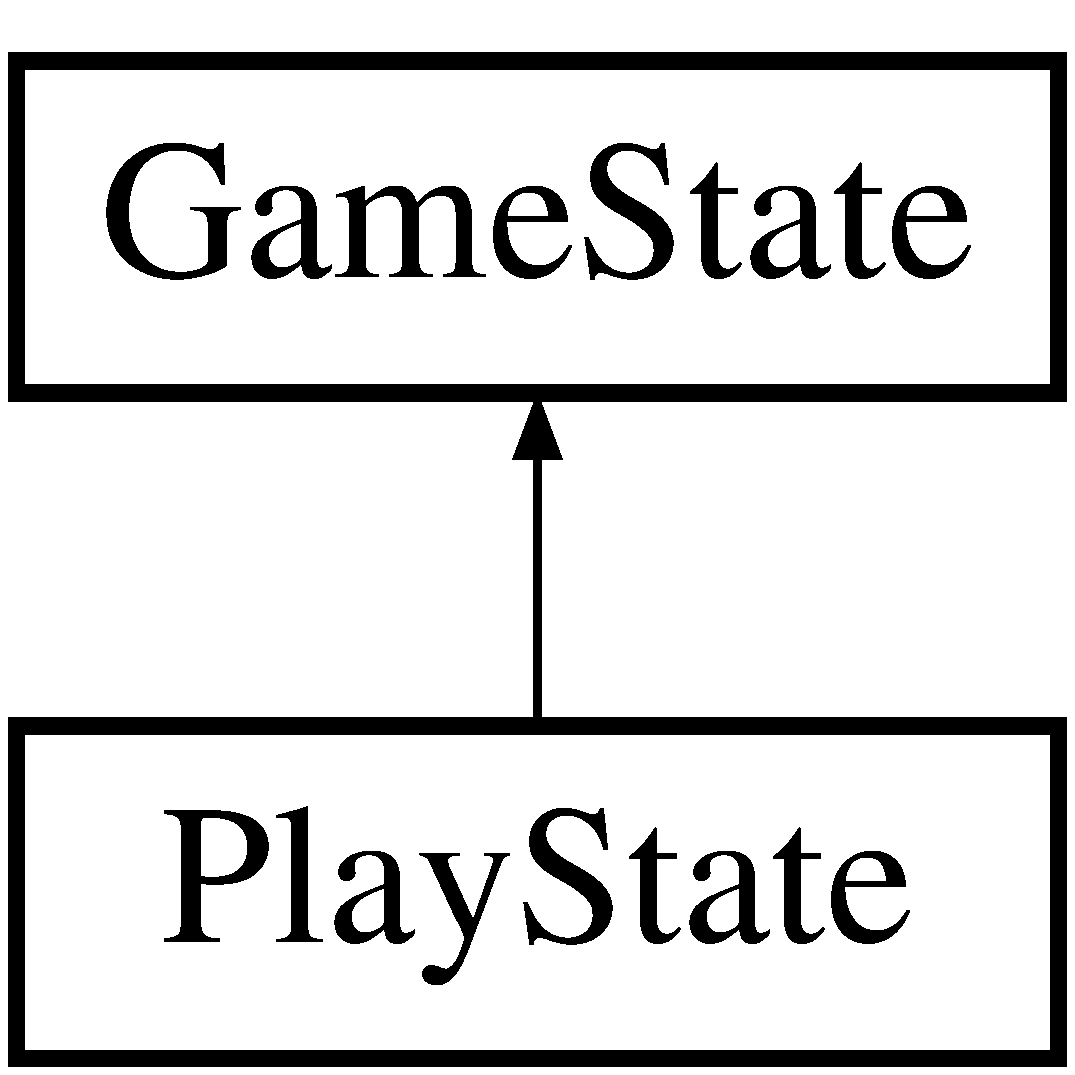
\includegraphics[height=2.000000cm]{class_play_state}
\end{center}
\end{figure}
\subsection*{Public Member Functions}
\begin{DoxyCompactItemize}
\item 
\hyperlink{class_play_state_a264b0ceb6dd2b120a2f1a4734dc4c672}{Play\+State} (S\+D\+L\+\_\+\+Window $\ast$win, S\+D\+L\+\_\+\+Renderer $\ast$rend)
\begin{DoxyCompactList}\small\item\em Constructor for \hyperlink{class_play_state}{Play\+State}. \end{DoxyCompactList}\item 
void \hyperlink{class_play_state_a3925fcdaebf7413fc5455dd306997a72}{init} ()
\begin{DoxyCompactList}\small\item\em Inititalizer for \hyperlink{class_play_state}{Play\+State}. \end{DoxyCompactList}\item 
void \hyperlink{class_play_state_af49af6d2bc865f0912a0c4e91f00de1a}{cleanup} ()
\begin{DoxyCompactList}\small\item\em Cleanup for \hyperlink{class_play_state}{Play\+State}. \end{DoxyCompactList}\item 
void \hyperlink{class_play_state_a981800722e3b0aba8ed05b18a52565d4}{load\+Level} (std\+::string level)
\begin{DoxyCompactList}\small\item\em Loads the objects from a .lvl file to the game field by calling create\+Object for every valid line. \end{DoxyCompactList}\item 
void \hyperlink{class_play_state_a02dd7375d2bfa61488a9854989aa5620}{create\+Object} (std\+::string name, int x, int y, int extra, std\+::string path, S\+D\+L\+\_\+\+Renderer $\ast$renderer)
\begin{DoxyCompactList}\small\item\em Creates an object on the game screen. \end{DoxyCompactList}\item 
void \hyperlink{class_play_state_ad9f095205941cd7ebd7d191a50a801d1}{update} (float const \&delta\+Time)
\begin{DoxyCompactList}\small\item\em Updater for \hyperlink{class_play_state}{Play\+State}. \end{DoxyCompactList}\item 
void \hyperlink{class_play_state_a892af1f154c3d789bb7f44e7a53e570f}{handle} (S\+D\+L\+\_\+\+Event event, float delta\+Time)
\begin{DoxyCompactList}\small\item\em Event handler for \hyperlink{class_play_state}{Play\+State}. \end{DoxyCompactList}\end{DoxyCompactItemize}
\subsection*{Additional Inherited Members}


\subsection{Constructor \& Destructor Documentation}
\hypertarget{class_play_state_a264b0ceb6dd2b120a2f1a4734dc4c672}{}\index{Play\+State@{Play\+State}!Play\+State@{Play\+State}}
\index{Play\+State@{Play\+State}!Play\+State@{Play\+State}}
\subsubsection[{Play\+State(\+S\+D\+L\+\_\+\+Window $\ast$win, S\+D\+L\+\_\+\+Renderer $\ast$rend)}]{\setlength{\rightskip}{0pt plus 5cm}Play\+State\+::\+Play\+State (
\begin{DoxyParamCaption}
\item[{S\+D\+L\+\_\+\+Window $\ast$}]{win, }
\item[{S\+D\+L\+\_\+\+Renderer $\ast$}]{rend}
\end{DoxyParamCaption}
)}\label{class_play_state_a264b0ceb6dd2b120a2f1a4734dc4c672}


Constructor for \hyperlink{class_play_state}{Play\+State}. 


\begin{DoxyParams}{Parameters}
{\em win} & window to draw to \\
\hline
{\em rend} & renderer to draw to \\
\hline
\end{DoxyParams}


\subsection{Member Function Documentation}
\hypertarget{class_play_state_af49af6d2bc865f0912a0c4e91f00de1a}{}\index{Play\+State@{Play\+State}!cleanup@{cleanup}}
\index{cleanup@{cleanup}!Play\+State@{Play\+State}}
\subsubsection[{cleanup()}]{\setlength{\rightskip}{0pt plus 5cm}void Play\+State\+::cleanup (
\begin{DoxyParamCaption}
{}
\end{DoxyParamCaption}
)\hspace{0.3cm}{\ttfamily [virtual]}}\label{class_play_state_af49af6d2bc865f0912a0c4e91f00de1a}


Cleanup for \hyperlink{class_play_state}{Play\+State}. 

Deletes every object in the game objects vector and the background. 

Implements \hyperlink{class_game_state}{Game\+State}.

\hypertarget{class_play_state_a02dd7375d2bfa61488a9854989aa5620}{}\index{Play\+State@{Play\+State}!create\+Object@{create\+Object}}
\index{create\+Object@{create\+Object}!Play\+State@{Play\+State}}
\subsubsection[{create\+Object(std\+::string name, int x, int y, int extra, std\+::string path, S\+D\+L\+\_\+\+Renderer $\ast$renderer)}]{\setlength{\rightskip}{0pt plus 5cm}void Play\+State\+::create\+Object (
\begin{DoxyParamCaption}
\item[{std\+::string}]{name, }
\item[{int}]{x, }
\item[{int}]{y, }
\item[{int}]{extra, }
\item[{std\+::string}]{path, }
\item[{S\+D\+L\+\_\+\+Renderer $\ast$}]{renderer}
\end{DoxyParamCaption}
)}\label{class_play_state_a02dd7375d2bfa61488a9854989aa5620}


Creates an object on the game screen. 

Creates the appropriate object depending on the name specified and pushes it to the game object vector. \hypertarget{class_play_state_a892af1f154c3d789bb7f44e7a53e570f}{}\index{Play\+State@{Play\+State}!handle@{handle}}
\index{handle@{handle}!Play\+State@{Play\+State}}
\subsubsection[{handle(\+S\+D\+L\+\_\+\+Event event, float delta\+Time)}]{\setlength{\rightskip}{0pt plus 5cm}void Play\+State\+::handle (
\begin{DoxyParamCaption}
\item[{S\+D\+L\+\_\+\+Event}]{event, }
\item[{float}]{delta\+Time}
\end{DoxyParamCaption}
)\hspace{0.3cm}{\ttfamily [virtual]}}\label{class_play_state_a892af1f154c3d789bb7f44e7a53e570f}


Event handler for \hyperlink{class_play_state}{Play\+State}. 

Fetches a pointer to the player from the game objects vector. Moves to menu state if escape is pressed. Moves player to new sublevel if applicable. Sends events to player event handler. 

Implements \hyperlink{class_game_state}{Game\+State}.

\hypertarget{class_play_state_a3925fcdaebf7413fc5455dd306997a72}{}\index{Play\+State@{Play\+State}!init@{init}}
\index{init@{init}!Play\+State@{Play\+State}}
\subsubsection[{init()}]{\setlength{\rightskip}{0pt plus 5cm}void Play\+State\+::init (
\begin{DoxyParamCaption}
{}
\end{DoxyParamCaption}
)\hspace{0.3cm}{\ttfamily [virtual]}}\label{class_play_state_a3925fcdaebf7413fc5455dd306997a72}


Inititalizer for \hyperlink{class_play_state}{Play\+State}. 

Loads and draws the background image for the play state. Loads the chosen level. 

Implements \hyperlink{class_game_state}{Game\+State}.

\hypertarget{class_play_state_a981800722e3b0aba8ed05b18a52565d4}{}\index{Play\+State@{Play\+State}!load\+Level@{load\+Level}}
\index{load\+Level@{load\+Level}!Play\+State@{Play\+State}}
\subsubsection[{load\+Level(std\+::string level)}]{\setlength{\rightskip}{0pt plus 5cm}void Play\+State\+::load\+Level (
\begin{DoxyParamCaption}
\item[{std\+::string}]{level}
\end{DoxyParamCaption}
)}\label{class_play_state_a981800722e3b0aba8ed05b18a52565d4}


Loads the objects from a .lvl file to the game field by calling create\+Object for every valid line. 

Clears the map objects vector and reserves enough space to hold all objects. Outputs a status message to the console. Initializes variables needed to create objects. Opens the level file. Uses stringstreams to load each line into the preivously created variables. Sends the variables to \hyperlink{class_play_state_a02dd7375d2bfa61488a9854989aa5620}{create\+Object()} if the object is valid. Creates borders around the game screen. \hypertarget{class_play_state_ad9f095205941cd7ebd7d191a50a801d1}{}\index{Play\+State@{Play\+State}!update@{update}}
\index{update@{update}!Play\+State@{Play\+State}}
\subsubsection[{update(float const \&delta\+Time)}]{\setlength{\rightskip}{0pt plus 5cm}void Play\+State\+::update (
\begin{DoxyParamCaption}
\item[{float const \&}]{delta\+Time}
\end{DoxyParamCaption}
)\hspace{0.3cm}{\ttfamily [virtual]}}\label{class_play_state_ad9f095205941cd7ebd7d191a50a801d1}


Updater for \hyperlink{class_play_state}{Play\+State}. 

Clears the screen. Draws the background. Loops through every object on the game screen. If an object is moving, check for collision with it and every other object. Create projectiles for object if applicable. Update object. Draw object in the correct direction. Move to deathstate if player dies. Move to menustate if player finishes game. Delete object. 

Implements \hyperlink{class_game_state}{Game\+State}.



The documentation for this class was generated from the following files\+:\begin{DoxyCompactItemize}
\item 
/\+Users/lukas.\+vikstrom/\+Documents/\+T\+D\+P005/\+T\+D\+P005-\/\+Projekt/Play\+State.\+h\item 
/\+Users/lukas.\+vikstrom/\+Documents/\+T\+D\+P005/\+T\+D\+P005-\/\+Projekt/Play\+State.\+cc\end{DoxyCompactItemize}

\hypertarget{class_projectile}{}\section{Projectile Class Reference}
\label{class_projectile}\index{Projectile@{Projectile}}
Inheritance diagram for Projectile\+:\begin{figure}[H]
\begin{center}
\leavevmode
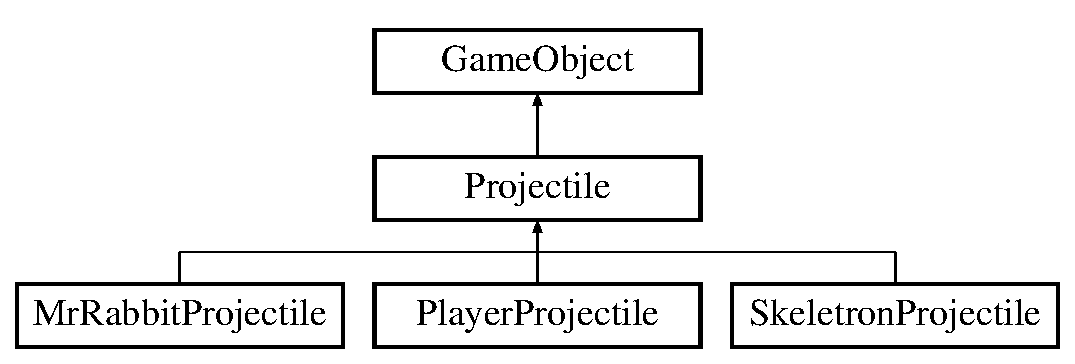
\includegraphics[height=3.000000cm]{class_projectile}
\end{center}
\end{figure}
\subsection*{Public Member Functions}
\begin{DoxyCompactItemize}
\item 
\hyperlink{class_projectile_afadf6ea4be9118e7af9dbe3f9d64e3ca}{Projectile} (int x\+\_\+p, int y\+\_\+p, int w, int h, int amount\+Of\+Frames, std\+::string sprite\+Sheet, S\+D\+L\+\_\+\+Renderer $\ast$render, int dir, \hyperlink{class_game_object}{Game\+Object} $\ast$creator\+\_\+ptr)
\begin{DoxyCompactList}\small\item\em Constructor for \hyperlink{class_game_object}{Game\+Object}. \end{DoxyCompactList}\item 
\hypertarget{class_projectile_a2bcd6e71abdfb70d278e90bff9be5f76}{}virtual void {\bfseries handle\+Collision} (std\+::vector$<$ std\+::pair$<$ \hyperlink{class_game_object}{Game\+Object} $\ast$, std\+::array$<$ std\+::string, 4 $>$$>$$>$ colliding\+Objects)\label{class_projectile_a2bcd6e71abdfb70d278e90bff9be5f76}

\item 
void \hyperlink{class_projectile_adf4854afefc6fdc8efbeb0f8e50b589c}{update} (float const \&delta\+Time)
\begin{DoxyCompactList}\small\item\em Updator for Projecile. \end{DoxyCompactList}\item 
void \hyperlink{class_projectile_aa6148f7507c5971232c1030db87c6aa7}{will\+Collide} (std\+::vector$<$ \hyperlink{class_game_object}{Game\+Object} $\ast$ $>$ const \&objects)
\begin{DoxyCompactList}\small\item\em Checks for collision with every object on the screen and handles it if collision has occurred. \end{DoxyCompactList}\end{DoxyCompactItemize}
\subsection*{Additional Inherited Members}


\subsection{Constructor \& Destructor Documentation}
\hypertarget{class_projectile_afadf6ea4be9118e7af9dbe3f9d64e3ca}{}\index{Projectile@{Projectile}!Projectile@{Projectile}}
\index{Projectile@{Projectile}!Projectile@{Projectile}}
\subsubsection[{Projectile(int x\+\_\+p, int y\+\_\+p, int w, int h, int amount\+Of\+Frames, std\+::string sprite\+Sheet, S\+D\+L\+\_\+\+Renderer $\ast$render, int dir, Game\+Object $\ast$creator\+\_\+ptr)}]{\setlength{\rightskip}{0pt plus 5cm}Projectile\+::\+Projectile (
\begin{DoxyParamCaption}
\item[{int}]{x\+\_\+p, }
\item[{int}]{y\+\_\+p, }
\item[{int}]{w, }
\item[{int}]{h, }
\item[{int}]{amount\+Of\+Frames, }
\item[{std\+::string}]{sprite\+Sheet, }
\item[{S\+D\+L\+\_\+\+Renderer $\ast$}]{render, }
\item[{int}]{dir, }
\item[{{\bf Game\+Object} $\ast$}]{creator\+\_\+ptr}
\end{DoxyParamCaption}
)}\label{class_projectile_afadf6ea4be9118e7af9dbe3f9d64e3ca}


Constructor for \hyperlink{class_game_object}{Game\+Object}. 


\begin{DoxyParams}{Parameters}
{\em x\+\_\+p} & x position of block \\
\hline
{\em y\+\_\+p} & y position of block \\
\hline
{\em w} & width of block \\
\hline
{\em h} & height of block \\
\hline
{\em amount\+Of\+Frames} & amount of frames in blocks spritesheet \\
\hline
{\em sprite\+Sheet} & location of spritesheet \\
\hline
{\em render} & renderer to draw to \\
\hline
{\em dir} & direction to spawn the projectile in \\
\hline
{\em creator\+\_\+ptr} & pointer to object that created projectile \\
\hline
\end{DoxyParams}


\subsection{Member Function Documentation}
\hypertarget{class_projectile_adf4854afefc6fdc8efbeb0f8e50b589c}{}\index{Projectile@{Projectile}!update@{update}}
\index{update@{update}!Projectile@{Projectile}}
\subsubsection[{update(float const \&delta\+Time)}]{\setlength{\rightskip}{0pt plus 5cm}void Projectile\+::update (
\begin{DoxyParamCaption}
\item[{float const \&}]{delta\+Time}
\end{DoxyParamCaption}
)\hspace{0.3cm}{\ttfamily [virtual]}}\label{class_projectile_adf4854afefc6fdc8efbeb0f8e50b589c}


Updator for Projecile. 

Resets collision during this update bool. Updates position of projectile. 

Implements \hyperlink{class_game_object}{Game\+Object}.

\hypertarget{class_projectile_aa6148f7507c5971232c1030db87c6aa7}{}\index{Projectile@{Projectile}!will\+Collide@{will\+Collide}}
\index{will\+Collide@{will\+Collide}!Projectile@{Projectile}}
\subsubsection[{will\+Collide(std\+::vector$<$ Game\+Object $\ast$ $>$ const \&objects)}]{\setlength{\rightskip}{0pt plus 5cm}void Projectile\+::will\+Collide (
\begin{DoxyParamCaption}
\item[{std\+::vector$<$ {\bf Game\+Object} $\ast$ $>$ const \&}]{objects}
\end{DoxyParamCaption}
)\hspace{0.3cm}{\ttfamily [virtual]}}\label{class_projectile_aa6148f7507c5971232c1030db87c6aa7}


Checks for collision with every object on the screen and handles it if collision has occurred. 

Creates a vector that will contain the object and the type of the object it collides with. Creates a vector with the resulting collision direction of the object it collides with. Loops through all objects on screen and checks for collision. Calls handle\+Collision() with the previously mentioned vector containing the object and its type. 

Implements \hyperlink{class_game_object}{Game\+Object}.



The documentation for this class was generated from the following files\+:\begin{DoxyCompactItemize}
\item 
/\+Users/lukas.\+vikstrom/\+Documents/\+T\+D\+P005/\+T\+D\+P005-\/\+Projekt/Projectile.\+h\item 
/\+Users/lukas.\+vikstrom/\+Documents/\+T\+D\+P005/\+T\+D\+P005-\/\+Projekt/Projectile.\+cc\end{DoxyCompactItemize}

\hypertarget{class_skeletron}{}\section{Skeletron Class Reference}
\label{class_skeletron}\index{Skeletron@{Skeletron}}
Inheritance diagram for Skeletron\+:\begin{figure}[H]
\begin{center}
\leavevmode
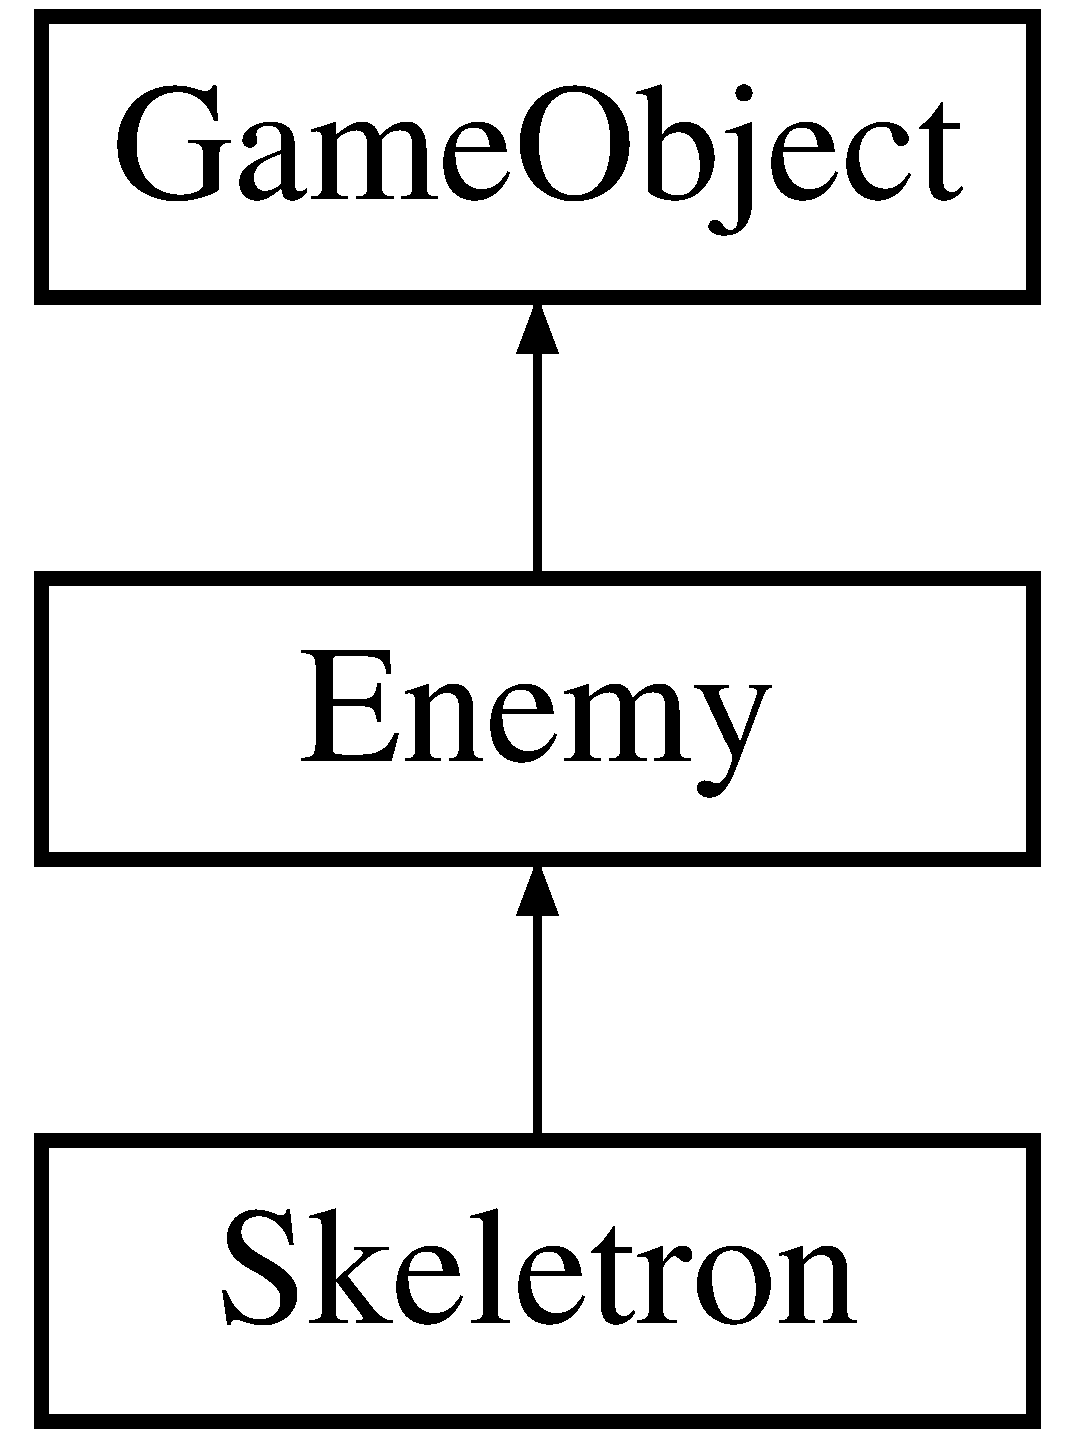
\includegraphics[height=3.000000cm]{class_skeletron}
\end{center}
\end{figure}
\subsection*{Public Member Functions}
\begin{DoxyCompactItemize}
\item 
\hyperlink{class_skeletron_acec7ab73ebcaa43fa6699a6b0216144a}{Skeletron} (int x\+\_\+pos, int y\+\_\+pos, S\+D\+L\+\_\+\+Renderer $\ast$render, \hyperlink{class_player}{Player} $\ast$player\+\_\+ptr, \hyperlink{class_active_block}{Active\+Block} $\ast$target\+\_\+obj)
\begin{DoxyCompactList}\small\item\em Constructor for \hyperlink{class_skeletron}{Skeletron}. \end{DoxyCompactList}\item 
\hyperlink{class_skeletron_a38931afc89baf959cfdfbd1d80205f5f}{$\sim$\+Skeletron} ()
\begin{DoxyCompactList}\small\item\em Deconstructor for \hyperlink{class_skeletron}{Skeletron}. \end{DoxyCompactList}\item 
void \hyperlink{class_skeletron_a71229cc19b0069069572564e6ea0083d}{update} (float const \&delta\+Time)
\begin{DoxyCompactList}\small\item\em Updator for \hyperlink{class_skeletron}{Skeletron}. \end{DoxyCompactList}\item 
void \hyperlink{class_skeletron_a624590dc55199a067fda03bc5ef05bc1}{decide\+Action} ()
\begin{DoxyCompactList}\small\item\em Decision making for \hyperlink{class_skeletron}{Skeletron}. \end{DoxyCompactList}\item 
void \hyperlink{class_skeletron_a536f37f0ea61bfb05805226148d683be}{create\+Object} (std\+::vector$<$ \hyperlink{class_game_object}{Game\+Object} $\ast$ $>$ \&map\+\_\+objects)
\begin{DoxyCompactList}\small\item\em \hyperlink{class_projectile}{Projectile} creation for \hyperlink{class_skeletron}{Skeletron}. \end{DoxyCompactList}\item 
void \hyperlink{class_skeletron_a581c47e082d196b8d7d09305404a67e8}{will\+Collide} (std\+::vector$<$ \hyperlink{class_game_object}{Game\+Object} $\ast$ $>$ const \&objects)
\begin{DoxyCompactList}\small\item\em Checks for collision with every object on the screen and handles it if collision has occurred. \end{DoxyCompactList}\end{DoxyCompactItemize}
\subsection*{Additional Inherited Members}


\subsection{Constructor \& Destructor Documentation}
\hypertarget{class_skeletron_acec7ab73ebcaa43fa6699a6b0216144a}{}\index{Skeletron@{Skeletron}!Skeletron@{Skeletron}}
\index{Skeletron@{Skeletron}!Skeletron@{Skeletron}}
\subsubsection[{Skeletron(int x\+\_\+pos, int y\+\_\+pos, S\+D\+L\+\_\+\+Renderer $\ast$render, Player $\ast$player\+\_\+ptr, Active\+Block $\ast$target\+\_\+obj)}]{\setlength{\rightskip}{0pt plus 5cm}Skeletron\+::\+Skeletron (
\begin{DoxyParamCaption}
\item[{int}]{x\+\_\+pos, }
\item[{int}]{y\+\_\+pos, }
\item[{S\+D\+L\+\_\+\+Renderer $\ast$}]{render, }
\item[{{\bf Player} $\ast$}]{player\+\_\+ptr, }
\item[{{\bf Active\+Block} $\ast$}]{target\+\_\+obj}
\end{DoxyParamCaption}
)}\label{class_skeletron_acec7ab73ebcaa43fa6699a6b0216144a}


Constructor for \hyperlink{class_skeletron}{Skeletron}. 


\begin{DoxyParams}{Parameters}
{\em x\+Pos} & x position of mr. rabbit \\
\hline
{\em y\+Pos} & y position of mr. rabbit \\
\hline
{\em render} & renderer to draw to \\
\hline
{\em player\+\_\+ptr} & pointer to active player \\
\hline
{\em target\+\_\+obj} & object to activate on death \\
\hline
\end{DoxyParams}
\hypertarget{class_skeletron_a38931afc89baf959cfdfbd1d80205f5f}{}\index{Skeletron@{Skeletron}!````~Skeletron@{$\sim$\+Skeletron}}
\index{````~Skeletron@{$\sim$\+Skeletron}!Skeletron@{Skeletron}}
\subsubsection[{$\sim$\+Skeletron()}]{\setlength{\rightskip}{0pt plus 5cm}Skeletron\+::$\sim$\+Skeletron (
\begin{DoxyParamCaption}
{}
\end{DoxyParamCaption}
)}\label{class_skeletron_a38931afc89baf959cfdfbd1d80205f5f}


Deconstructor for \hyperlink{class_skeletron}{Skeletron}. 

Deletes the pointer data members. 

\subsection{Member Function Documentation}
\hypertarget{class_skeletron_a536f37f0ea61bfb05805226148d683be}{}\index{Skeletron@{Skeletron}!create\+Object@{create\+Object}}
\index{create\+Object@{create\+Object}!Skeletron@{Skeletron}}
\subsubsection[{create\+Object(std\+::vector$<$ Game\+Object $\ast$ $>$ \&map\+\_\+objects)}]{\setlength{\rightskip}{0pt plus 5cm}void Skeletron\+::create\+Object (
\begin{DoxyParamCaption}
\item[{std\+::vector$<$ {\bf Game\+Object} $\ast$ $>$ \&}]{map\+\_\+objects}
\end{DoxyParamCaption}
)\hspace{0.3cm}{\ttfamily [virtual]}}\label{class_skeletron_a536f37f0ea61bfb05805226148d683be}


\hyperlink{class_projectile}{Projectile} creation for \hyperlink{class_skeletron}{Skeletron}. 

Creates skeletrons projectile if he is able to shoot and then resets the variable related to shooting. 

Reimplemented from \hyperlink{class_game_object}{Game\+Object}.

\hypertarget{class_skeletron_a624590dc55199a067fda03bc5ef05bc1}{}\index{Skeletron@{Skeletron}!decide\+Action@{decide\+Action}}
\index{decide\+Action@{decide\+Action}!Skeletron@{Skeletron}}
\subsubsection[{decide\+Action()}]{\setlength{\rightskip}{0pt plus 5cm}void Skeletron\+::decide\+Action (
\begin{DoxyParamCaption}
{}
\end{DoxyParamCaption}
)\hspace{0.3cm}{\ttfamily [virtual]}}\label{class_skeletron_a624590dc55199a067fda03bc5ef05bc1}


Decision making for \hyperlink{class_skeletron}{Skeletron}. 

If the player is nearby or a 1 in 200 chance occurs it will initialize a teleport. Changes direction depending on the players position. Determines where to shoot the projectile depending on the players y position. 

Implements \hyperlink{class_enemy}{Enemy}.

\hypertarget{class_skeletron_a71229cc19b0069069572564e6ea0083d}{}\index{Skeletron@{Skeletron}!update@{update}}
\index{update@{update}!Skeletron@{Skeletron}}
\subsubsection[{update(float const \&delta\+Time)}]{\setlength{\rightskip}{0pt plus 5cm}void Skeletron\+::update (
\begin{DoxyParamCaption}
\item[{float const \&}]{delta\+Time}
\end{DoxyParamCaption}
)\hspace{0.3cm}{\ttfamily [virtual]}}\label{class_skeletron_a71229cc19b0069069572564e6ea0083d}


Updator for \hyperlink{class_skeletron}{Skeletron}. 

Calculates and draws the health bar. Activates target object if dying. Draws the teleport indicator if a teleport is imminent and adds time to the time until teleport. Teleports if its time to teleport. Decides action. Updates x position. Updates y position. 

Implements \hyperlink{class_game_object}{Game\+Object}.

\hypertarget{class_skeletron_a581c47e082d196b8d7d09305404a67e8}{}\index{Skeletron@{Skeletron}!will\+Collide@{will\+Collide}}
\index{will\+Collide@{will\+Collide}!Skeletron@{Skeletron}}
\subsubsection[{will\+Collide(std\+::vector$<$ Game\+Object $\ast$ $>$ const \&objects)}]{\setlength{\rightskip}{0pt plus 5cm}void Skeletron\+::will\+Collide (
\begin{DoxyParamCaption}
\item[{std\+::vector$<$ {\bf Game\+Object} $\ast$ $>$ const \&}]{objects}
\end{DoxyParamCaption}
)\hspace{0.3cm}{\ttfamily [virtual]}}\label{class_skeletron_a581c47e082d196b8d7d09305404a67e8}


Checks for collision with every object on the screen and handles it if collision has occurred. 

Creates a vector that will contain the object and the type of the object it collides with. Creates a vector with the resulting collision direction of the object it collides with. Loops through all objects on screen and checks for collision. Calls handle\+Collision() with the previously mentioned vector containing the object and its type. 

Implements \hyperlink{class_game_object}{Game\+Object}.



The documentation for this class was generated from the following files\+:\begin{DoxyCompactItemize}
\item 
/\+Users/lukas.\+vikstrom/\+Documents/\+T\+D\+P005/\+T\+D\+P005-\/\+Projekt/Skeletron.\+h\item 
/\+Users/lukas.\+vikstrom/\+Documents/\+T\+D\+P005/\+T\+D\+P005-\/\+Projekt/Skeletron.\+cc\end{DoxyCompactItemize}

\hypertarget{class_skeletron_projectile}{}\section{Skeletron\+Projectile Class Reference}
\label{class_skeletron_projectile}\index{Skeletron\+Projectile@{Skeletron\+Projectile}}
Inheritance diagram for Skeletron\+Projectile\+:\begin{figure}[H]
\begin{center}
\leavevmode
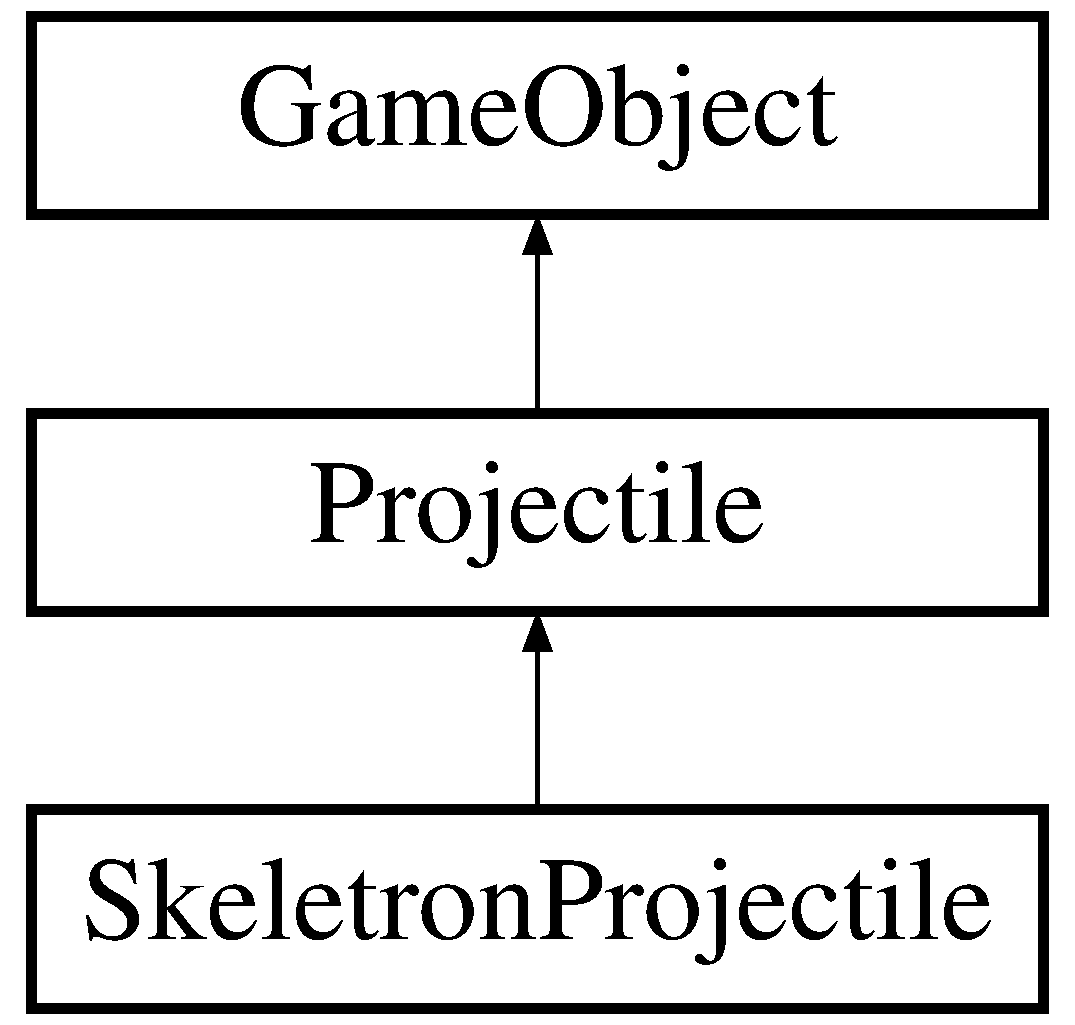
\includegraphics[height=3.000000cm]{class_skeletron_projectile}
\end{center}
\end{figure}
\subsection*{Public Member Functions}
\begin{DoxyCompactItemize}
\item 
\hyperlink{class_skeletron_projectile_ab8c5623726cf166d0220ac69d8bfbc1a}{Skeletron\+Projectile} (int x, int y, int dir\+X, int dir\+Y, S\+D\+L\+\_\+\+Renderer $\ast$render, \hyperlink{class_game_object}{Game\+Object} $\ast$creator\+\_\+ptr)
\begin{DoxyCompactList}\small\item\em Constructor for \hyperlink{class_skeletron_projectile}{Skeletron\+Projectile}. \end{DoxyCompactList}\end{DoxyCompactItemize}
\subsection*{Additional Inherited Members}


\subsection{Constructor \& Destructor Documentation}
\hypertarget{class_skeletron_projectile_ab8c5623726cf166d0220ac69d8bfbc1a}{}\index{Skeletron\+Projectile@{Skeletron\+Projectile}!Skeletron\+Projectile@{Skeletron\+Projectile}}
\index{Skeletron\+Projectile@{Skeletron\+Projectile}!Skeletron\+Projectile@{Skeletron\+Projectile}}
\subsubsection[{Skeletron\+Projectile(int x, int y, int dir\+X, int dir\+Y, S\+D\+L\+\_\+\+Renderer $\ast$render, Game\+Object $\ast$creator\+\_\+ptr)}]{\setlength{\rightskip}{0pt plus 5cm}Skeletron\+Projectile\+::\+Skeletron\+Projectile (
\begin{DoxyParamCaption}
\item[{int}]{x, }
\item[{int}]{y, }
\item[{int}]{dir\+X, }
\item[{int}]{dir\+Y, }
\item[{S\+D\+L\+\_\+\+Renderer $\ast$}]{render, }
\item[{{\bf Game\+Object} $\ast$}]{creator\+\_\+ptr}
\end{DoxyParamCaption}
)}\label{class_skeletron_projectile_ab8c5623726cf166d0220ac69d8bfbc1a}


Constructor for \hyperlink{class_skeletron_projectile}{Skeletron\+Projectile}. 


\begin{DoxyParams}{Parameters}
{\em x} & x position of projectile \\
\hline
{\em y} & y position of projectile \\
\hline
{\em dir\+X} & x direction to spawn projectile in \\
\hline
{\em dir\+Y} & y direction to spawn projectile in \\
\hline
{\em render} & renderer to draw to \\
\hline
{\em creator\+\_\+ptr} & pointer to object that created projectile \\
\hline
\end{DoxyParams}


The documentation for this class was generated from the following files\+:\begin{DoxyCompactItemize}
\item 
/\+Users/lukas.\+vikstrom/\+Documents/\+T\+D\+P005/\+T\+D\+P005-\/\+Projekt/Skeletron\+Projectile.\+h\item 
/\+Users/lukas.\+vikstrom/\+Documents/\+T\+D\+P005/\+T\+D\+P005-\/\+Projekt/Skeletron\+Projectile.\+cc\end{DoxyCompactItemize}

\hypertarget{class_speed_demon}{}\section{Speed\+Demon Class Reference}
\label{class_speed_demon}\index{Speed\+Demon@{Speed\+Demon}}
Inheritance diagram for Speed\+Demon\+:\begin{figure}[H]
\begin{center}
\leavevmode
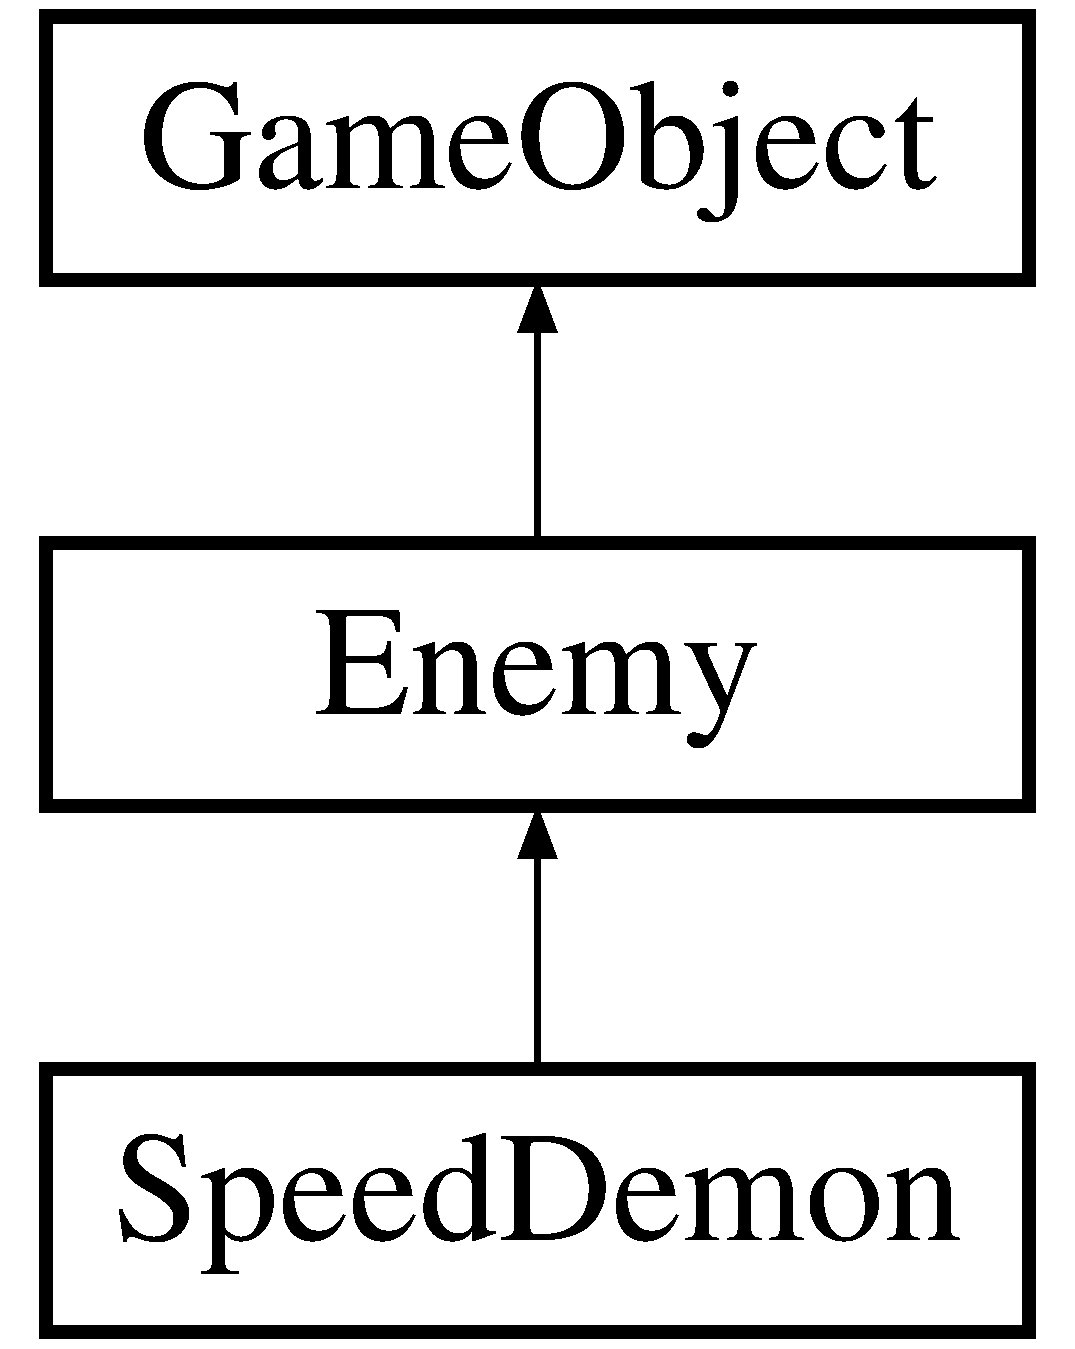
\includegraphics[height=3.000000cm]{class_speed_demon}
\end{center}
\end{figure}
\subsection*{Public Member Functions}
\begin{DoxyCompactItemize}
\item 
\hyperlink{class_speed_demon_a224e6ae33da2dd3471c0a83d26a3b23f}{Speed\+Demon} (int x\+\_\+pos, int y\+\_\+pos, S\+D\+L\+\_\+\+Renderer $\ast$render, \hyperlink{class_player}{Player} $\ast$player\+\_\+ptr)
\begin{DoxyCompactList}\small\item\em Constructor for \hyperlink{class_speed_demon}{Speed\+Demon}. \end{DoxyCompactList}\item 
\hypertarget{class_speed_demon_ac84b479a3261e6814aa551b403a78da4}{}void \hyperlink{class_speed_demon_ac84b479a3261e6814aa551b403a78da4}{update} (float const \&delta\+Time)\label{class_speed_demon_ac84b479a3261e6814aa551b403a78da4}

\begin{DoxyCompactList}\small\item\em Update function for \hyperlink{class_speed_demon}{Speed\+Demon}. \end{DoxyCompactList}\item 
void \hyperlink{class_speed_demon_aeae7a4127babf8a8bcc6e2c56512652a}{will\+Collide} (std\+::vector$<$ \hyperlink{class_game_object}{Game\+Object} $\ast$ $>$ const \&objects)
\begin{DoxyCompactList}\small\item\em Collision check for \hyperlink{class_speed_demon}{Speed\+Demon}. \end{DoxyCompactList}\item 
void \hyperlink{class_speed_demon_a36b21b02c91a92bd471b9de5975f7162}{decide\+Action} ()
\begin{DoxyCompactList}\small\item\em Calculates next action. \end{DoxyCompactList}\end{DoxyCompactItemize}
\subsection*{Additional Inherited Members}


\subsection{Constructor \& Destructor Documentation}
\hypertarget{class_speed_demon_a224e6ae33da2dd3471c0a83d26a3b23f}{}\index{Speed\+Demon@{Speed\+Demon}!Speed\+Demon@{Speed\+Demon}}
\index{Speed\+Demon@{Speed\+Demon}!Speed\+Demon@{Speed\+Demon}}
\subsubsection[{Speed\+Demon(int x\+\_\+pos, int y\+\_\+pos, S\+D\+L\+\_\+\+Renderer $\ast$render, Player $\ast$player\+\_\+ptr)}]{\setlength{\rightskip}{0pt plus 5cm}Speed\+Demon\+::\+Speed\+Demon (
\begin{DoxyParamCaption}
\item[{int}]{x\+\_\+pos, }
\item[{int}]{y\+\_\+pos, }
\item[{S\+D\+L\+\_\+\+Renderer $\ast$}]{render, }
\item[{{\bf Player} $\ast$}]{player\+\_\+ptr}
\end{DoxyParamCaption}
)}\label{class_speed_demon_a224e6ae33da2dd3471c0a83d26a3b23f}


Constructor for \hyperlink{class_speed_demon}{Speed\+Demon}. 


\begin{DoxyParams}{Parameters}
{\em x\+Pos} & x position of object \\
\hline
{\em y\+Pos} & y position of object \\
\hline
{\em player\+\_\+ptr} & pointer to extract its coordinates \\
\hline
{\em render} & renderer to draw to \\
\hline
\end{DoxyParams}


\subsection{Member Function Documentation}
\hypertarget{class_speed_demon_a36b21b02c91a92bd471b9de5975f7162}{}\index{Speed\+Demon@{Speed\+Demon}!decide\+Action@{decide\+Action}}
\index{decide\+Action@{decide\+Action}!Speed\+Demon@{Speed\+Demon}}
\subsubsection[{decide\+Action()}]{\setlength{\rightskip}{0pt plus 5cm}void Speed\+Demon\+::decide\+Action (
\begin{DoxyParamCaption}
{}
\end{DoxyParamCaption}
)\hspace{0.3cm}{\ttfamily [virtual]}}\label{class_speed_demon_a36b21b02c91a92bd471b9de5975f7162}


Calculates next action. 

If \hyperlink{class_player}{Player} x is to the left of object and difference in y is less than 100, move to the left. If \hyperlink{class_player}{Player} x is to the right of object and difference in y is less than 100, move to the right If \hyperlink{class_player}{Player} is not within reach or same x, stand still. 

Implements \hyperlink{class_enemy}{Enemy}.

\hypertarget{class_speed_demon_aeae7a4127babf8a8bcc6e2c56512652a}{}\index{Speed\+Demon@{Speed\+Demon}!will\+Collide@{will\+Collide}}
\index{will\+Collide@{will\+Collide}!Speed\+Demon@{Speed\+Demon}}
\subsubsection[{will\+Collide(std\+::vector$<$ Game\+Object $\ast$ $>$ const \&objects)}]{\setlength{\rightskip}{0pt plus 5cm}void Speed\+Demon\+::will\+Collide (
\begin{DoxyParamCaption}
\item[{std\+::vector$<$ {\bf Game\+Object} $\ast$ $>$ const \&}]{objects}
\end{DoxyParamCaption}
)\hspace{0.3cm}{\ttfamily [virtual]}}\label{class_speed_demon_aeae7a4127babf8a8bcc6e2c56512652a}


Collision check for \hyperlink{class_speed_demon}{Speed\+Demon}. 

Iterates the vector with objects in map and sends them to intersect 

Implements \hyperlink{class_game_object}{Game\+Object}.



The documentation for this class was generated from the following files\+:\begin{DoxyCompactItemize}
\item 
/\+Users/lukas.\+vikstrom/\+Documents/\+T\+D\+P005/\+T\+D\+P005-\/\+Projekt/Speed\+Demon.\+h\item 
/\+Users/lukas.\+vikstrom/\+Documents/\+T\+D\+P005/\+T\+D\+P005-\/\+Projekt/Speed\+Demon.\+cc\end{DoxyCompactItemize}

\hypertarget{class_spike_block}{}\section{Spike\+Block Class Reference}
\label{class_spike_block}\index{Spike\+Block@{Spike\+Block}}
Inheritance diagram for Spike\+Block\+:\begin{figure}[H]
\begin{center}
\leavevmode
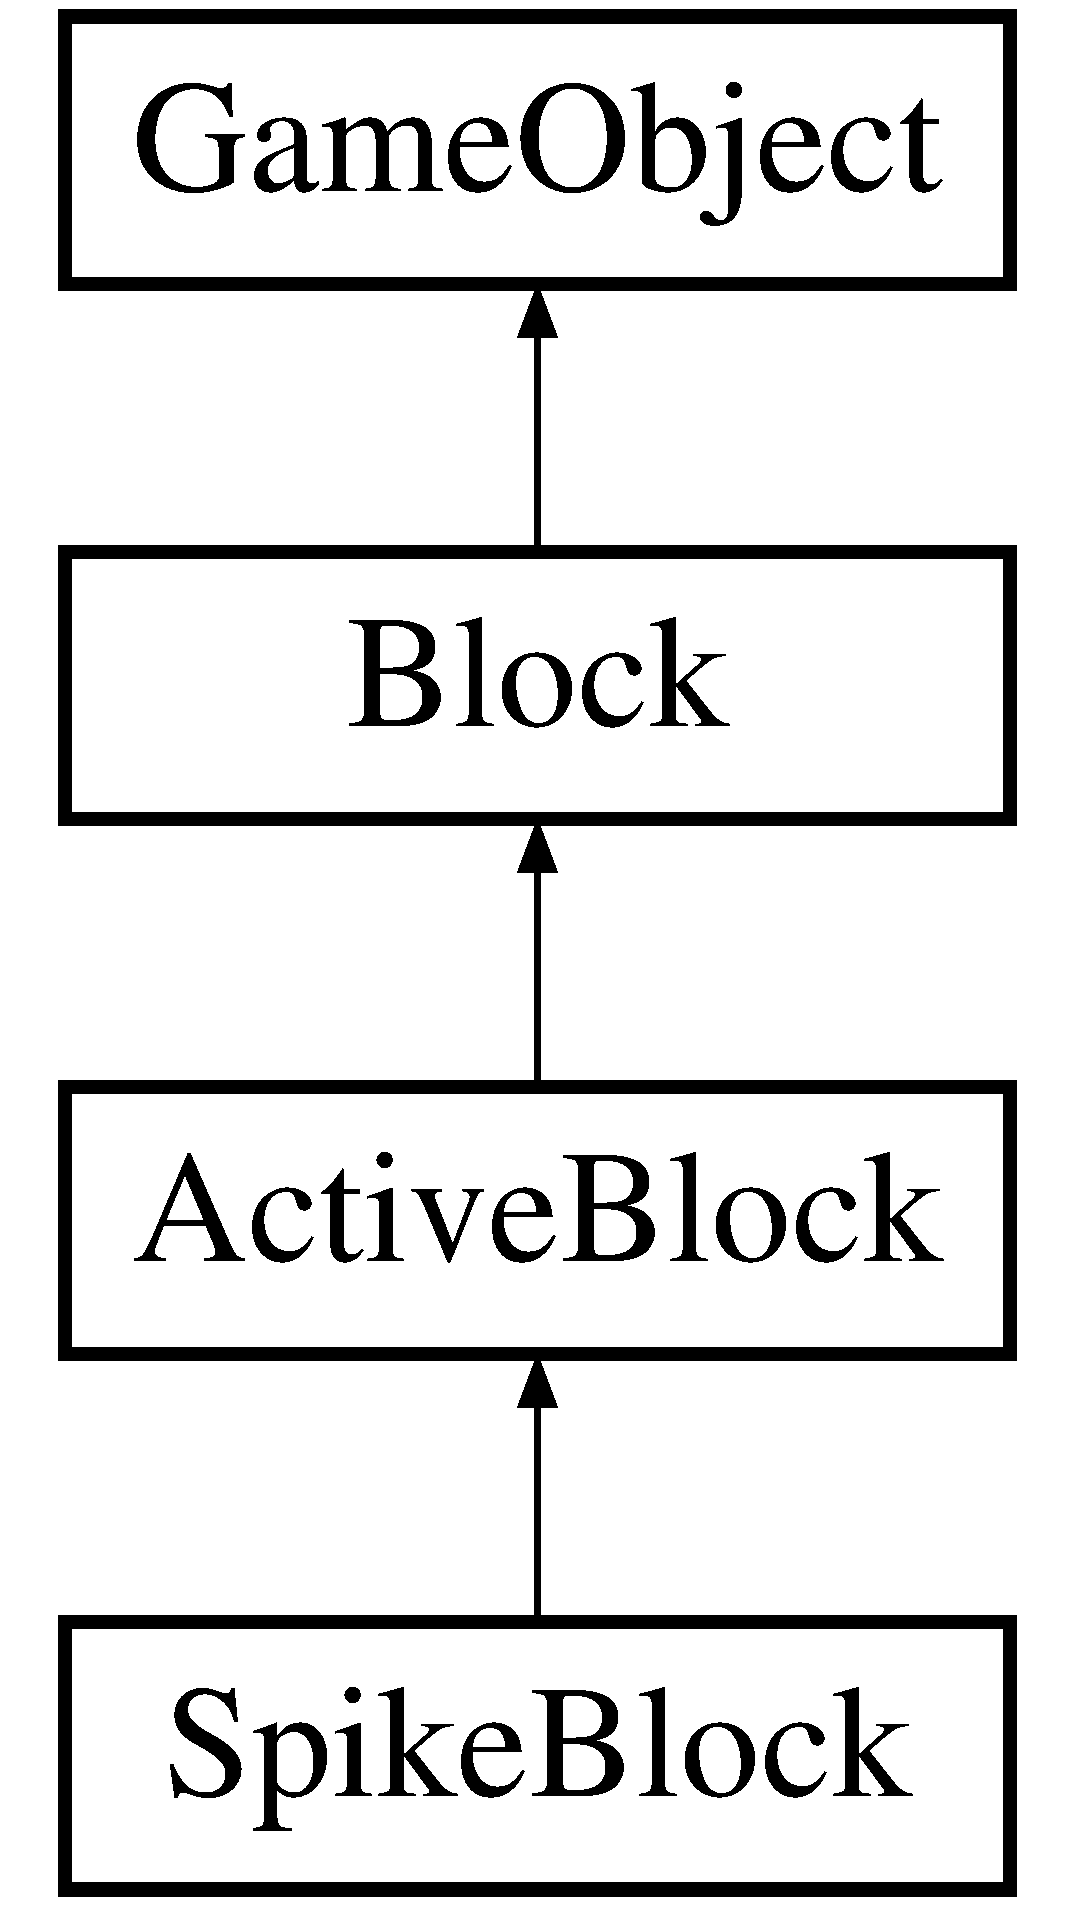
\includegraphics[height=4.000000cm]{class_spike_block}
\end{center}
\end{figure}
\subsection*{Public Member Functions}
\begin{DoxyCompactItemize}
\item 
\hyperlink{class_spike_block_aabeaf2df666bff3f84b7ad49088d3954}{Spike\+Block} (int x\+\_\+pos, int y\+\_\+pos, S\+D\+L\+\_\+\+Renderer $\ast$renderer, int acti)
\begin{DoxyCompactList}\small\item\em Constructor for \hyperlink{class_spike_block}{Spike\+Block}. \end{DoxyCompactList}\item 
void \hyperlink{class_spike_block_a7ade107c2b0c33d90c2743453761c220}{activate} ()
\begin{DoxyCompactList}\small\item\em Activate for \hyperlink{class_spike_block}{Spike\+Block}. \end{DoxyCompactList}\item 
\hypertarget{class_spike_block_a147f0fc4fba3f140e46d7d72496ada29}{}void \hyperlink{class_spike_block_a147f0fc4fba3f140e46d7d72496ada29}{de\+Activate} ()\label{class_spike_block_a147f0fc4fba3f140e46d7d72496ada29}

\begin{DoxyCompactList}\small\item\em Hides the \hyperlink{class_spike_block}{Spike\+Block}. \end{DoxyCompactList}\end{DoxyCompactItemize}
\subsection*{Additional Inherited Members}


\subsection{Constructor \& Destructor Documentation}
\hypertarget{class_spike_block_aabeaf2df666bff3f84b7ad49088d3954}{}\index{Spike\+Block@{Spike\+Block}!Spike\+Block@{Spike\+Block}}
\index{Spike\+Block@{Spike\+Block}!Spike\+Block@{Spike\+Block}}
\subsubsection[{Spike\+Block(int x\+\_\+pos, int y\+\_\+pos, S\+D\+L\+\_\+\+Renderer $\ast$renderer, int acti)}]{\setlength{\rightskip}{0pt plus 5cm}Spike\+Block\+::\+Spike\+Block (
\begin{DoxyParamCaption}
\item[{int}]{x\+\_\+pos, }
\item[{int}]{y\+\_\+pos, }
\item[{S\+D\+L\+\_\+\+Renderer $\ast$}]{renderer, }
\item[{int}]{acti}
\end{DoxyParamCaption}
)}\label{class_spike_block_aabeaf2df666bff3f84b7ad49088d3954}


Constructor for \hyperlink{class_spike_block}{Spike\+Block}. 


\begin{DoxyParams}{Parameters}
{\em x\+Pos} & x position of block \\
\hline
{\em y\+Pos} & y position of block \\
\hline
{\em render} & renderer to draw to \\
\hline
{\em active} & If the object should be visible at start \\
\hline
\end{DoxyParams}


\subsection{Member Function Documentation}
\hypertarget{class_spike_block_a7ade107c2b0c33d90c2743453761c220}{}\index{Spike\+Block@{Spike\+Block}!activate@{activate}}
\index{activate@{activate}!Spike\+Block@{Spike\+Block}}
\subsubsection[{activate()}]{\setlength{\rightskip}{0pt plus 5cm}void Spike\+Block\+::activate (
\begin{DoxyParamCaption}
{}
\end{DoxyParamCaption}
)\hspace{0.3cm}{\ttfamily [virtual]}}\label{class_spike_block_a7ade107c2b0c33d90c2743453761c220}


Activate for \hyperlink{class_spike_block}{Spike\+Block}. 

If the object at creation was set to be invisible, triggering via triggerblock will show it. If the object at creation was set to be visible, call de\+Activate function. 

Implements \hyperlink{class_active_block}{Active\+Block}.



The documentation for this class was generated from the following files\+:\begin{DoxyCompactItemize}
\item 
/\+Users/lukas.\+vikstrom/\+Documents/\+T\+D\+P005/\+T\+D\+P005-\/\+Projekt/Spike\+Block.\+h\item 
/\+Users/lukas.\+vikstrom/\+Documents/\+T\+D\+P005/\+T\+D\+P005-\/\+Projekt/Spike\+Block.\+cc\end{DoxyCompactItemize}

\hypertarget{class_sprite}{}\section{Sprite Class Reference}
\label{class_sprite}\index{Sprite@{Sprite}}
\subsection*{Public Member Functions}
\begin{DoxyCompactItemize}
\item 
\hyperlink{class_sprite_a7ae031c9623419893c010c4587a42d00}{Sprite} (int x\+\_\+p, int y\+\_\+p, int w, int h, int amount\+Of\+Frames, std\+::string sprite\+Sheet, S\+D\+L\+\_\+\+Renderer $\ast$render)
\begin{DoxyCompactList}\small\item\em Constructor for \hyperlink{class_sprite}{Sprite}. \end{DoxyCompactList}\item 
void \hyperlink{class_sprite_aa97420bd41d1f70eae5d0ec8c4e83b50}{draw} (int const \&direction)
\begin{DoxyCompactList}\small\item\em Draws the current object. \end{DoxyCompactList}\item 
void \hyperlink{class_sprite_a5e70e16bf7e519926dee9b96b71ae6a0}{update\+Animation} ()
\begin{DoxyCompactList}\small\item\em Updates the animation. \end{DoxyCompactList}\item 
void \hyperlink{class_sprite_a8c446bde8c4fc3e36252bbf2b26e2833}{load\+Sprite} ()
\begin{DoxyCompactList}\small\item\em Loads the sprite from given path. \end{DoxyCompactList}\item 
\hypertarget{class_sprite_abfc114955c893dc7d00b872eeb62ab59}{}void {\bfseries set\+Animation\+Current} (int const \&new\+Animation\+Frame)\label{class_sprite_abfc114955c893dc7d00b872eeb62ab59}

\item 
\hypertarget{class_sprite_af12c44d4b19efdaa6ce51e1fcad8b086}{}void {\bfseries set\+Animation\+Progress} (int const \&new\+Animation\+Frame)\label{class_sprite_af12c44d4b19efdaa6ce51e1fcad8b086}

\item 
\hypertarget{class_sprite_aaa7d9a9582651ff62dcb4a051926c342}{}void {\bfseries set\+Animation\+Start\+Index} (int const \&new\+Animation\+Frame)\label{class_sprite_aaa7d9a9582651ff62dcb4a051926c342}

\item 
\hypertarget{class_sprite_a064d0e14144921c39451debf65962e38}{}void {\bfseries set\+Animation\+End\+Index} (int const \&new\+Animation\+Frame)\label{class_sprite_a064d0e14144921c39451debf65962e38}

\item 
\hypertarget{class_sprite_a45ec693b97cb6b47473c1f2de9cb53ed}{}int {\bfseries get\+Animation\+Current} () const \label{class_sprite_a45ec693b97cb6b47473c1f2de9cb53ed}

\item 
\hypertarget{class_sprite_ab62a139516184d4fb110eed77f3e8f83}{}int {\bfseries get\+Animation\+Progress} () const \label{class_sprite_ab62a139516184d4fb110eed77f3e8f83}

\item 
\hypertarget{class_sprite_a296fabe394ccef7082b7af187b06c96e}{}int {\bfseries get\+Animation\+Start\+Index} () const \label{class_sprite_a296fabe394ccef7082b7af187b06c96e}

\item 
\hypertarget{class_sprite_a1aae49d75fa10b382297a9d9d54a83e0}{}int {\bfseries get\+Animation\+End\+Index} () const \label{class_sprite_a1aae49d75fa10b382297a9d9d54a83e0}

\item 
\hypertarget{class_sprite_aaaadb46aa25f6eec1e6ee4b19540e835}{}S\+D\+L\+\_\+\+Renderer $\ast$ {\bfseries get\+Renderer} () const \label{class_sprite_aaaadb46aa25f6eec1e6ee4b19540e835}

\end{DoxyCompactItemize}
\subsection*{Public Attributes}
\begin{DoxyCompactItemize}
\item 
\hypertarget{class_sprite_a531ed274733d916261f49e1a2cbb6ba9}{}S\+D\+L\+\_\+\+Texture $\ast$ {\bfseries texture}\label{class_sprite_a531ed274733d916261f49e1a2cbb6ba9}

\item 
\hypertarget{class_sprite_ae10dc2e1909783c117cb9247d7484ee3}{}S\+D\+L\+\_\+\+Rect {\bfseries sprite\+Clips} \mbox{[}8\mbox{]}\label{class_sprite_ae10dc2e1909783c117cb9247d7484ee3}

\item 
\hypertarget{class_sprite_a8c0a36cf84c36b2882622d51f79914db}{}S\+D\+L\+\_\+\+Rect {\bfseries sprite\+Rect}\label{class_sprite_a8c0a36cf84c36b2882622d51f79914db}

\end{DoxyCompactItemize}


\subsection{Constructor \& Destructor Documentation}
\hypertarget{class_sprite_a7ae031c9623419893c010c4587a42d00}{}\index{Sprite@{Sprite}!Sprite@{Sprite}}
\index{Sprite@{Sprite}!Sprite@{Sprite}}
\subsubsection[{Sprite(int x\+\_\+p, int y\+\_\+p, int w, int h, int amount\+Of\+Frames, std\+::string sprite\+Sheet, S\+D\+L\+\_\+\+Renderer $\ast$render)}]{\setlength{\rightskip}{0pt plus 5cm}Sprite\+::\+Sprite (
\begin{DoxyParamCaption}
\item[{int}]{x\+\_\+p, }
\item[{int}]{y\+\_\+p, }
\item[{int}]{w, }
\item[{int}]{h, }
\item[{int}]{amount\+Of\+Frames, }
\item[{std\+::string}]{sprite\+Sheet, }
\item[{S\+D\+L\+\_\+\+Renderer $\ast$}]{render}
\end{DoxyParamCaption}
)}\label{class_sprite_a7ae031c9623419893c010c4587a42d00}


Constructor for \hyperlink{class_sprite}{Sprite}. 


\begin{DoxyParams}{Parameters}
{\em x\+\_\+p} & x position of object \\
\hline
{\em y\+\_\+p} & y position of object \\
\hline
{\em w} & width of each animation frame \\
\hline
{\em h} & height of each animation frame \\
\hline
{\em amount\+Of\+Frames} & amount of frames in blocks spritesheet \\
\hline
{\em sprite\+Sheet} & location of spritesheet \\
\hline
{\em render} & renderer to draw to \\
\hline
\end{DoxyParams}


\subsection{Member Function Documentation}
\hypertarget{class_sprite_aa97420bd41d1f70eae5d0ec8c4e83b50}{}\index{Sprite@{Sprite}!draw@{draw}}
\index{draw@{draw}!Sprite@{Sprite}}
\subsubsection[{draw(int const \&direction)}]{\setlength{\rightskip}{0pt plus 5cm}void Sprite\+::draw (
\begin{DoxyParamCaption}
\item[{int const \&}]{direction}
\end{DoxyParamCaption}
)}\label{class_sprite_aa97420bd41d1f70eae5d0ec8c4e83b50}


Draws the current object. 

Depending on the objects direction, draws a flipped image \hypertarget{class_sprite_a8c446bde8c4fc3e36252bbf2b26e2833}{}\index{Sprite@{Sprite}!load\+Sprite@{load\+Sprite}}
\index{load\+Sprite@{load\+Sprite}!Sprite@{Sprite}}
\subsubsection[{load\+Sprite()}]{\setlength{\rightskip}{0pt plus 5cm}void Sprite\+::load\+Sprite (
\begin{DoxyParamCaption}
{}
\end{DoxyParamCaption}
)}\label{class_sprite_a8c446bde8c4fc3e36252bbf2b26e2833}


Loads the sprite from given path. 

Converts the image to and Texture$\ast$ via Surface$\ast$ Creates spriteclips depending on size and height of sprite\+Rect \hypertarget{class_sprite_a5e70e16bf7e519926dee9b96b71ae6a0}{}\index{Sprite@{Sprite}!update\+Animation@{update\+Animation}}
\index{update\+Animation@{update\+Animation}!Sprite@{Sprite}}
\subsubsection[{update\+Animation()}]{\setlength{\rightskip}{0pt plus 5cm}void Sprite\+::update\+Animation (
\begin{DoxyParamCaption}
{}
\end{DoxyParamCaption}
)}\label{class_sprite_a5e70e16bf7e519926dee9b96b71ae6a0}


Updates the animation. 

Depending on the current animation and how many animation it contains, it resets the animation value animation\+Current is used to specifiy which parts of the spritesheet to display 

The documentation for this class was generated from the following files\+:\begin{DoxyCompactItemize}
\item 
/\+Users/lukas.\+vikstrom/\+Documents/\+T\+D\+P005/\+T\+D\+P005-\/\+Projekt/Sprite.\+h\item 
/\+Users/lukas.\+vikstrom/\+Documents/\+T\+D\+P005/\+T\+D\+P005-\/\+Projekt/Sprite.\+cc\end{DoxyCompactItemize}

\hypertarget{class_state_machine}{}\section{State\+Machine Class Reference}
\label{class_state_machine}\index{State\+Machine@{State\+Machine}}
\subsection*{Public Member Functions}
\begin{DoxyCompactItemize}
\item 
void \hyperlink{class_state_machine_aa5e0d6f0b06376d0357af0ff85b5b9b2}{init} ()
\begin{DoxyCompactList}\small\item\em Initializer for \hyperlink{class_state_machine}{State\+Machine}. \end{DoxyCompactList}\item 
void \hyperlink{class_state_machine_a64f96b117421c50e208e5c40724230ed}{cleanup} ()
\begin{DoxyCompactList}\small\item\em Cleaner for \hyperlink{class_state_machine}{State\+Machine}. \end{DoxyCompactList}\item 
void \hyperlink{class_state_machine_a408fa50a60a9cff42124df913fbbe69e}{change\+State} (\hyperlink{class_game_state}{Game\+State} $\ast$state)
\begin{DoxyCompactList}\small\item\em State changer \hyperlink{class_state_machine}{State\+Machine}. \end{DoxyCompactList}\item 
\hypertarget{class_state_machine_a129876e0f4cc92f2319ea309244e713a}{}\hyperlink{class_game_state}{Game\+State} $\ast$ {\bfseries get\+Current\+State} ()\label{class_state_machine_a129876e0f4cc92f2319ea309244e713a}

\item 
void \hyperlink{class_state_machine_abc3ca328b644f3d2c557fd04ccd65ddd}{update} ()
\begin{DoxyCompactList}\small\item\em Calls current gamestates update function. \end{DoxyCompactList}\end{DoxyCompactItemize}


\subsection{Member Function Documentation}
\hypertarget{class_state_machine_a408fa50a60a9cff42124df913fbbe69e}{}\index{State\+Machine@{State\+Machine}!change\+State@{change\+State}}
\index{change\+State@{change\+State}!State\+Machine@{State\+Machine}}
\subsubsection[{change\+State(\+Game\+State $\ast$state)}]{\setlength{\rightskip}{0pt plus 5cm}void State\+Machine\+::change\+State (
\begin{DoxyParamCaption}
\item[{{\bf Game\+State} $\ast$}]{new\+State}
\end{DoxyParamCaption}
)}\label{class_state_machine_a408fa50a60a9cff42124df913fbbe69e}


State changer \hyperlink{class_state_machine}{State\+Machine}. 

Switches the member variable current\+State to the gamestate pointer Initializes the new gamestate \hypertarget{class_state_machine_a64f96b117421c50e208e5c40724230ed}{}\index{State\+Machine@{State\+Machine}!cleanup@{cleanup}}
\index{cleanup@{cleanup}!State\+Machine@{State\+Machine}}
\subsubsection[{cleanup()}]{\setlength{\rightskip}{0pt plus 5cm}void State\+Machine\+::cleanup (
\begin{DoxyParamCaption}
{}
\end{DoxyParamCaption}
)}\label{class_state_machine_a64f96b117421c50e208e5c40724230ed}


Cleaner for \hyperlink{class_state_machine}{State\+Machine}. 

Deallocates the different gamestates Deletes the Window Deletes the renderer \hypertarget{class_state_machine_aa5e0d6f0b06376d0357af0ff85b5b9b2}{}\index{State\+Machine@{State\+Machine}!init@{init}}
\index{init@{init}!State\+Machine@{State\+Machine}}
\subsubsection[{init()}]{\setlength{\rightskip}{0pt plus 5cm}void State\+Machine\+::init (
\begin{DoxyParamCaption}
{}
\end{DoxyParamCaption}
)}\label{class_state_machine_aa5e0d6f0b06376d0357af0ff85b5b9b2}


Initializer for \hyperlink{class_state_machine}{State\+Machine}. 

Creates windows with S\+C\+R\+E\+E\+N\+\_\+\+W\+I\+D\+T\+H and S\+C\+R\+E\+E\+N\+\_\+\+H\+E\+I\+G\+H\+T Creates a renderer to use for drawing Creates the different gamestates and adds them to a vector Changes the current state to display the menu Calls update for the current state \hypertarget{class_state_machine_abc3ca328b644f3d2c557fd04ccd65ddd}{}\index{State\+Machine@{State\+Machine}!update@{update}}
\index{update@{update}!State\+Machine@{State\+Machine}}
\subsubsection[{update()}]{\setlength{\rightskip}{0pt plus 5cm}void State\+Machine\+::update (
\begin{DoxyParamCaption}
{}
\end{DoxyParamCaption}
)}\label{class_state_machine_abc3ca328b644f3d2c557fd04ccd65ddd}


Calls current gamestates update function. 

Calculates the time between frames Calls update function in the current gamestate with delta\+Time as parameter 

The documentation for this class was generated from the following files\+:\begin{DoxyCompactItemize}
\item 
/\+Users/lukas.\+vikstrom/\+Documents/\+T\+D\+P005/\+T\+D\+P005-\/\+Projekt/State\+Machine.\+h\item 
/\+Users/lukas.\+vikstrom/\+Documents/\+T\+D\+P005/\+T\+D\+P005-\/\+Projekt/State\+Machine.\+cc\end{DoxyCompactItemize}

\hypertarget{class_trigger_block}{}\section{Trigger\+Block Class Reference}
\label{class_trigger_block}\index{Trigger\+Block@{Trigger\+Block}}
Inheritance diagram for Trigger\+Block\+:\begin{figure}[H]
\begin{center}
\leavevmode
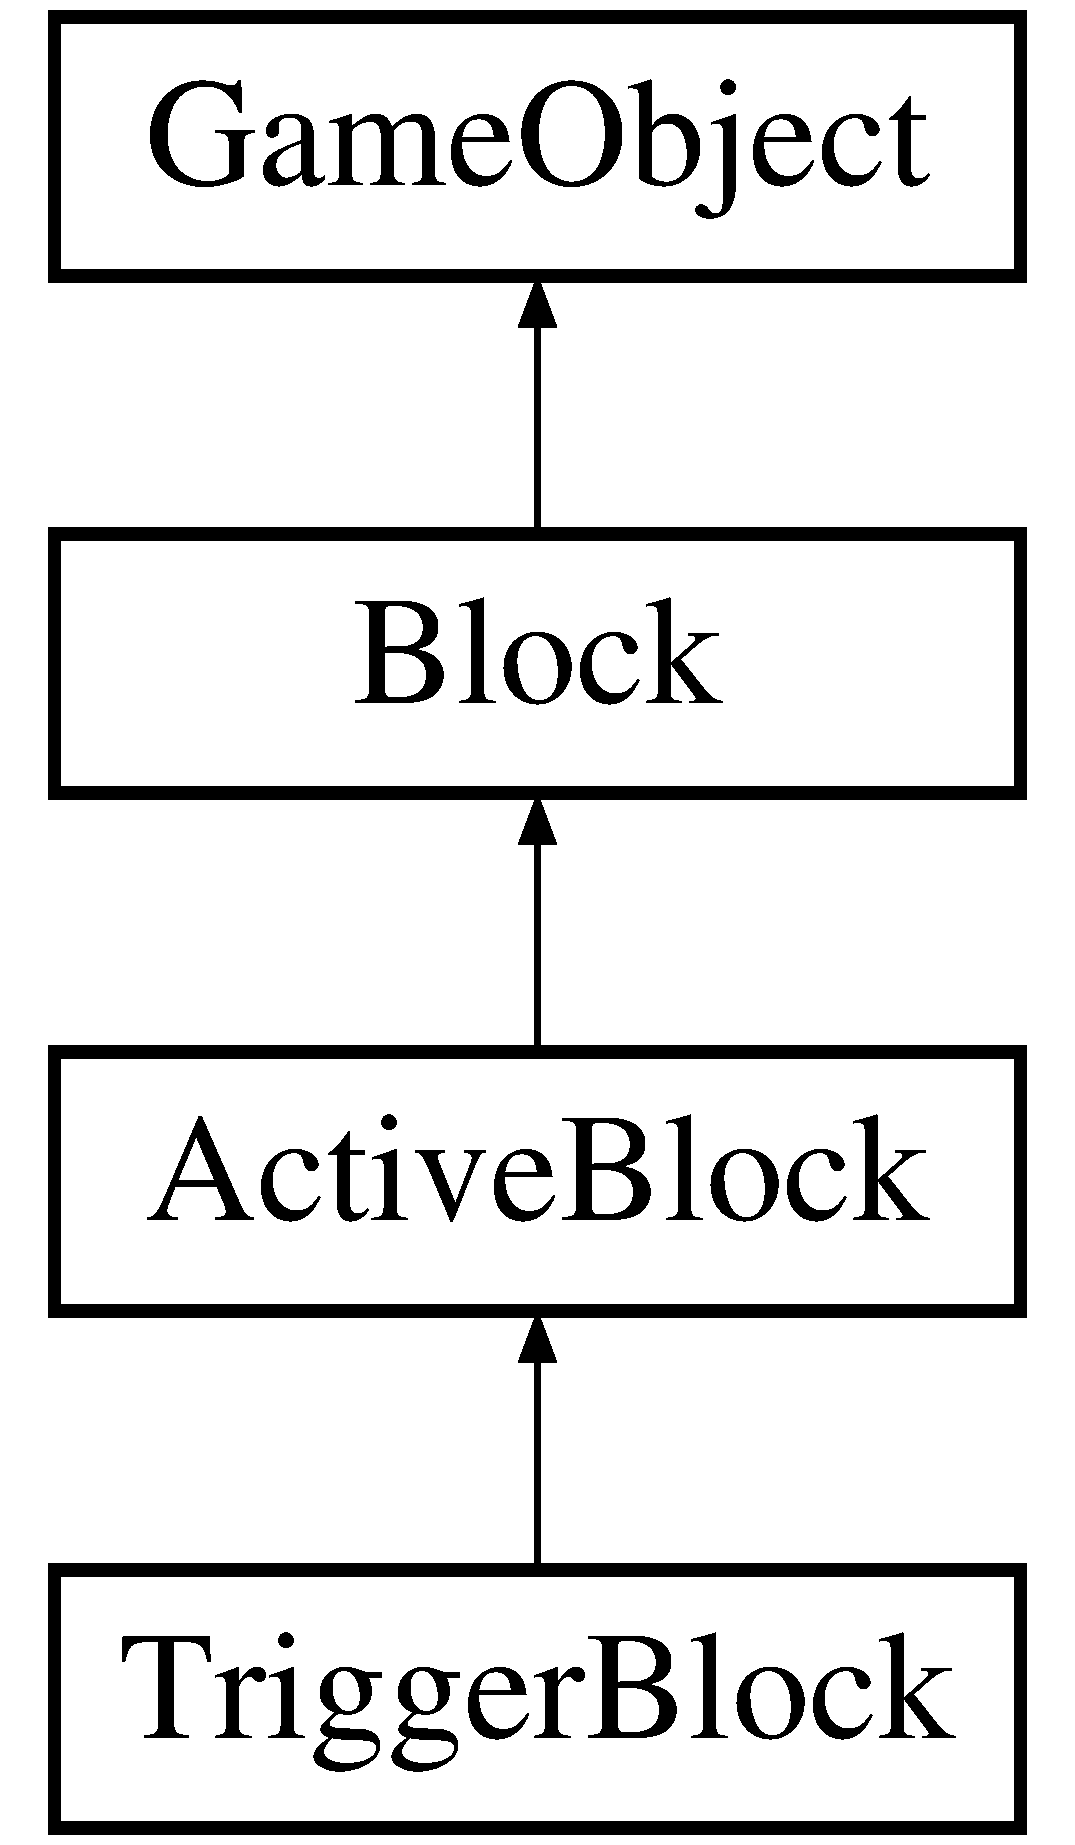
\includegraphics[height=4.000000cm]{class_trigger_block}
\end{center}
\end{figure}
\subsection*{Public Member Functions}
\begin{DoxyCompactItemize}
\item 
\hyperlink{class_trigger_block_ab80e0e8f0ab696180a40d343aa2c7788}{Trigger\+Block} (int x\+\_\+pos, int y\+\_\+pos, S\+D\+L\+\_\+\+Renderer $\ast$renderer, \hyperlink{class_active_block}{Active\+Block} $\ast$target\+\_\+obj)
\begin{DoxyCompactList}\small\item\em Constructor for \hyperlink{class_trigger_block}{Trigger\+Block}. \end{DoxyCompactList}\item 
\hypertarget{class_trigger_block_afe2b4404380a69686dee246083cd0447}{}void \hyperlink{class_trigger_block_afe2b4404380a69686dee246083cd0447}{activate} ()\label{class_trigger_block_afe2b4404380a69686dee246083cd0447}

\begin{DoxyCompactList}\small\item\em Activator for \hyperlink{class_trigger_block}{Trigger\+Block} Calls the target objects activate function. \end{DoxyCompactList}\end{DoxyCompactItemize}
\subsection*{Additional Inherited Members}


\subsection{Constructor \& Destructor Documentation}
\hypertarget{class_trigger_block_ab80e0e8f0ab696180a40d343aa2c7788}{}\index{Trigger\+Block@{Trigger\+Block}!Trigger\+Block@{Trigger\+Block}}
\index{Trigger\+Block@{Trigger\+Block}!Trigger\+Block@{Trigger\+Block}}
\subsubsection[{Trigger\+Block(int x\+\_\+pos, int y\+\_\+pos, S\+D\+L\+\_\+\+Renderer $\ast$renderer, Active\+Block $\ast$target\+\_\+obj)}]{\setlength{\rightskip}{0pt plus 5cm}Trigger\+Block\+::\+Trigger\+Block (
\begin{DoxyParamCaption}
\item[{int}]{x\+\_\+pos, }
\item[{int}]{y\+\_\+pos, }
\item[{S\+D\+L\+\_\+\+Renderer $\ast$}]{renderer, }
\item[{{\bf Active\+Block} $\ast$}]{target\+\_\+obj}
\end{DoxyParamCaption}
)}\label{class_trigger_block_ab80e0e8f0ab696180a40d343aa2c7788}


Constructor for \hyperlink{class_trigger_block}{Trigger\+Block}. 


\begin{DoxyParams}{Parameters}
{\em x\+Pos} & x position of block \\
\hline
{\em y\+Pos} & y position of block \\
\hline
{\em render} & renderer to draw to \\
\hline
{\em target\+\_\+obj} & Pointer to object which the trigger will activate. \\
\hline
\end{DoxyParams}


The documentation for this class was generated from the following files\+:\begin{DoxyCompactItemize}
\item 
/\+Users/lukas.\+vikstrom/\+Documents/\+T\+D\+P005/\+T\+D\+P005-\/\+Projekt/Trigger\+Block.\+h\item 
/\+Users/lukas.\+vikstrom/\+Documents/\+T\+D\+P005/\+T\+D\+P005-\/\+Projekt/Trigger\+Block.\+cc\end{DoxyCompactItemize}

%--- End generated contents ---

% Index
\backmatter
\newpage
\phantomsection
\clearemptydoublepage
\addcontentsline{toc}{chapter}{Index}
\printindex

\end{document}
